\documentclass[czech]{book}
\usepackage{babel}

\usepackage{geometry}
 \geometry{
 a5paper,
 left=12mm,
 top=10mm,
 right=12mm,
 bottom=14mm,
 }

\pagestyle{plain}

\usepackage{etoolbox}
\makeatletter
\patchcmd{\chapter}{\if@openright\cleardoublepage\else\clearpage\fi}{}{}{}
\makeatother


\usepackage[utf8]{inputenc}
\usepackage[T1]{fontenc}
\usepackage{PTSerif}

\usepackage{titlesec}
\usepackage{multicol}
\usepackage{bookmark}


\titleformat{\chapter}[display]
  {\normalfont\bfseries}{}{0pt}{\Large}

\titlespacing*{\chapter}{0pt}{0pt}{20pt}

\usepackage{graphicx}
\usepackage{pdfpages}
\usepackage{wrapfig}

\newcommand*\podpis[1]{
	\vspace*{1pt} 
	\hspace*{0em plus 1fill}\makebox{\textbf{#1}}
	\vspace*{12pt} 
}

\newcommand{\nopar}{{\parfillskip=0pt \par}}



\begin{document}

%
\begin{titlepage}
	\centering

	\vspace*{0.2\textheight} 

	{\LARGE Kniha KEYA} % Author name
	
	\vspace*{0.05\textheight} 
	
	\textbf{\LARGE 2019}\\[\baselineskip] % First title line
	
	
	\vfill
	

\end{titlepage}


\includepdf[pages={1}]{img/obal.pdf}

\newgeometry{left=25mm,right=25mm}

\chapter{Předmluva} % (fold)
\label{cha:předmluva}

Milá Keyačko, milý Keyáku,
držíš v rukou knihu Keya. V potocích kolem tábořišť uteklo už mnoho vody (snad kromě toho posledního chudáka) od doby, kdy jsi držel tu předchozí. To, aby se Kniha Keya stala skutečností, není úplně jednoduchá záležitost, ale letos…

Píše se 21. listopadu 2019 a skupina bláznivých nadšenců se ujala příprav Knihy Keya. A aby to nebylo jen tak, rozhodla se, že Knihu Keyu představí veřejnosti na vánočním večírku. Měla necelý měsíc a volnou ruku. Je tedy vcelku pochopitelné, že ustoupila od megalomanských mnohastránkových projektů a rozhodla se pro minimalistickou verzi, již právě držíš.

Letos máš opět možnost se nad mísou cukroví a s hrnkem čaje (nebo driáku?) začíst a zavzpomínat (mimojiné) na slunečné, ale málo sněhové hory v Mařenicích, na stavebku plnou práce, ale zároveň smíchu a samozřejmě na tábor. Krom toho najdeš v knize i mnohé další zajímavé články a na konci, na konci je překvapení!

Tak tedy, krásné Vánoce a pěkné počtení
přeje za letošní hvězdný KKtým

\restoregeometry

% chapter předmluva (end)
\clearpage
\newgeometry{left=30mm,right=30mm}

\tableofcontents

\restoregeometry
\clearpage
\pagebreak
\pagebreak
\clearpage

\chapter{Lodní deník Anpetu} % (fold)
\label{cha:lodní_deník_etapkové_skupiny_černí_rytíři_anpetu_}

Šest námořních posádek na táboře Anpetu si mělo po celou dobu plavby za pokladem vést lodní deník, přičemž na konci tábora byly deníky vybrány a zhodnoceny. Zde předkládáme úplný přepis deníku posádky Černí rytíři. Z původního deníku pochází třeba i inkonzistence psaní data.


\label{sub:lodní_deník_etapkové_skupiny_černí_rytíři}

% subsection lodní_deník_etapkové_skupiny_černí_rytíři (end)

\subsubsection{Neděle 7. 7. 2019, rozdělování do etapek} % (fold)
\label{ssub:rozdělování_do_etapek}

% subsubsection rozdělování_do_etapek (end)
Dopoledne jsme se rozdělovali do etapkových skupinek. Chodili jsme po různých stanovištích kde jsme plnili úkoly, jako třeba vytahování barelu s vodou ze skoro vyschlého potoka, nebo lezení na strom.

Na jednom stanovišti se vyplňoval dotazník, na kterém byly otázky jako třeba kolik šupin mám mořská panna, jak to, že si někdo umí spolknout nos a různé jiné námořnické otázky...
Potom jsme chvíli pracovali.

...A pak jsme dostali tenhle sešit do skupinekm které rozdělila kapitánka lodi, na které poplujeme, Kukumbrie drsné oko. V naší skupince jsou Hanuš, Zub, Anežka, Mauglí, Holub a Grizzly.

\podpis{Anežka}

\begin{center}
	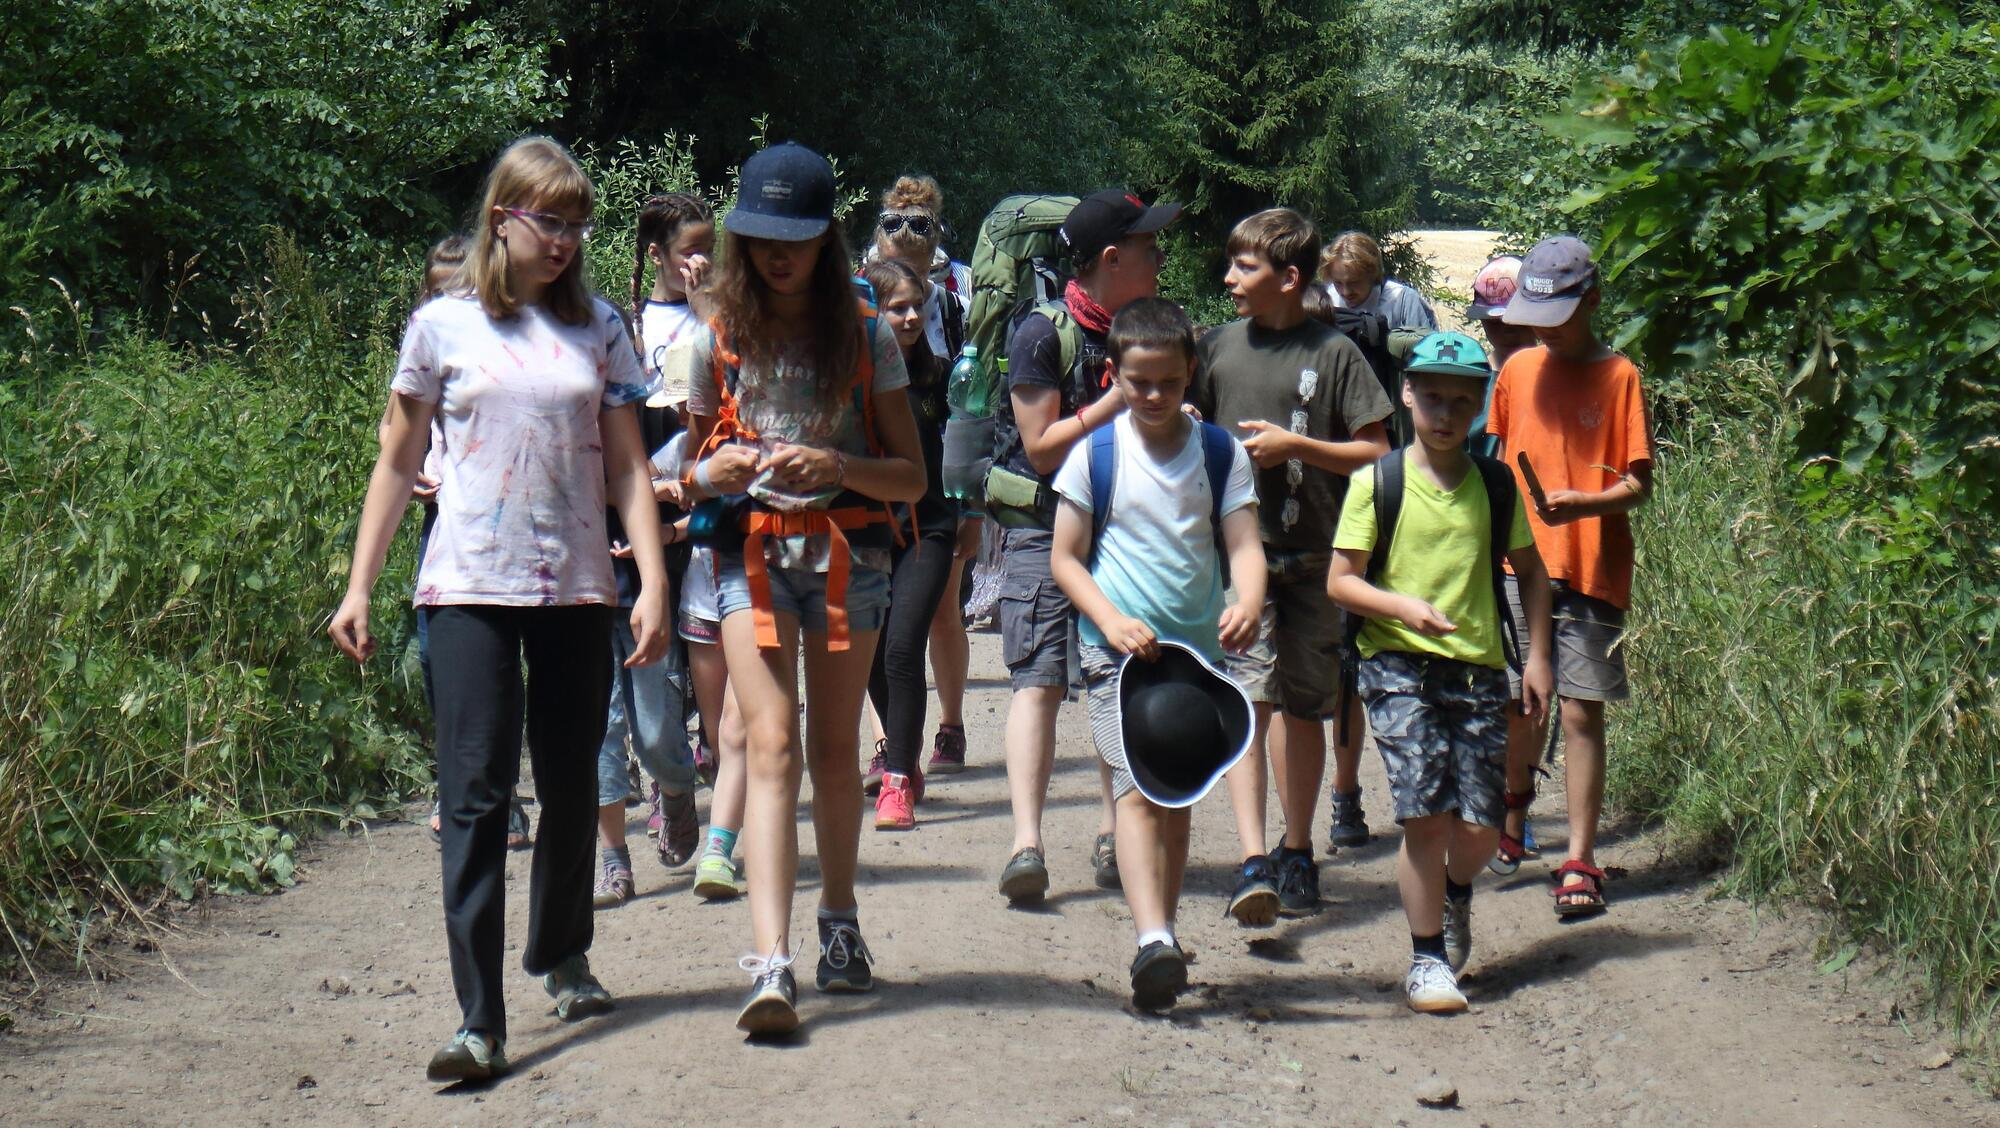
\includegraphics[width=12cm]{img/anpetu_tabor/prichod.JPG}
\end{center}


\subsubsection{Pondělí 8. 7. 2019 - Etapková hra} % (fold)
\label{ssub:pondělí_8_7_2019_etapková_hra}

% subsubsection pondělí_8_7_2019_etapková_hra (end)

Dnes jsme hráli velmi zajímavou hru. Šlo o to že jsme běhali po několika stanovištích, a získávali jsme suroviny které jsme zase prodali ale za víc a za ty peníze co jsme získali jsme museli zase něco koupit například maso, zrní, zelí a tak dále museli jsme toho získat hodně a ještě získat peněz ale vyplatilo se to a vypráli jsme první místo dostali jsme dost peněz na to abychom si koupili například děla, koš (námořnický) a další věci

\podpis{GRIZZLY}

\begin{center}
	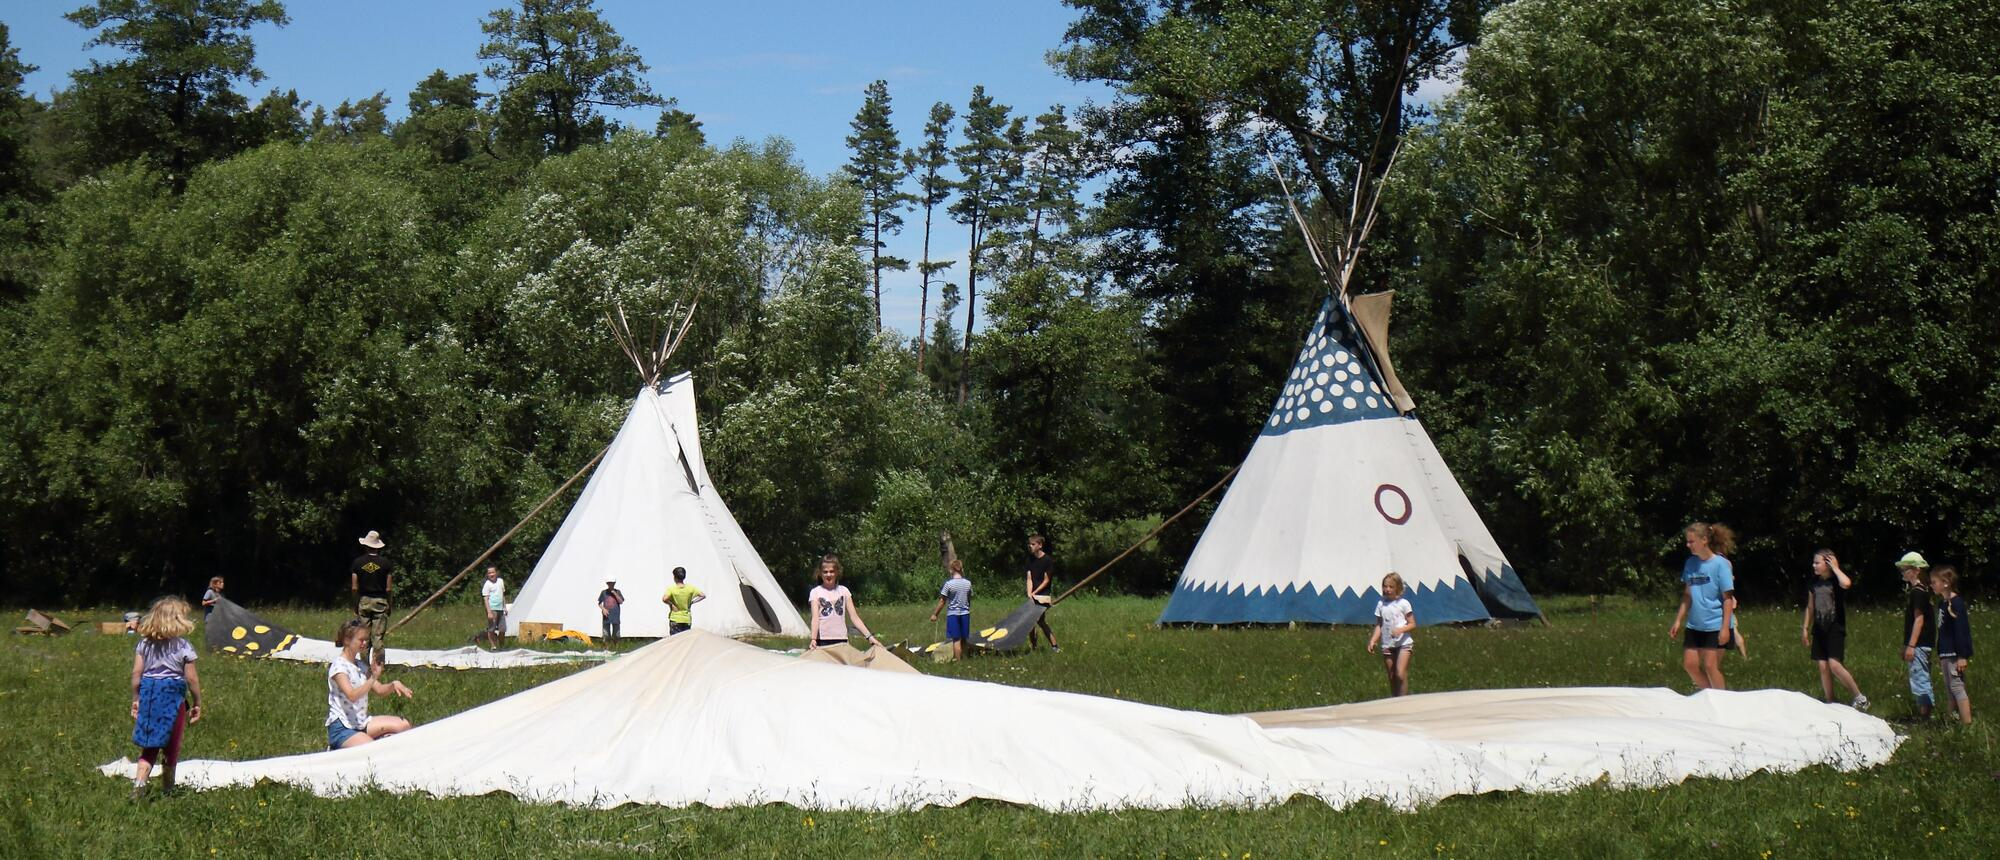
\includegraphics[width=12cm]{img/anpetu_tabor/typka.JPG}
\end{center}


\subsubsection{Úterý 9. 7. 2019 - 2. Etapková hra } % (fold)
\label{ssub:_9_7_2019_2_etapková_hra_}


Odpoledne nám Uďové řekli, abychom se oblíkli do plavek a přes ně si dali kostýmy. Když jsme to udělali, šli jsme k rybníku, kde jsme se rozdělili na etapkové skupinky a dostali jsme nafukovací matračku.

Když se začalo, měli jsme matračku nafouknout a postupně na ni vždy plavat asi do půlky rybníkukde byly balónky naší skupinky.

Každý pak měl prasknout jeden balónek a plavat zpátky...
Nakonec jsme skončili první spolu se skupinkou Žraloci, protože jsme byli úplně nastejno.

\podpis{Anežka}
% subsubsection _9_7_2019_2_etapková_hra_ (end)



\subsubsection{Středa 10. 7 - Úterý 11. 7. 2019 - 3. Etapková hra} % (fold)
\label{ssub:3_etapková_hra}

Takže, ve středu večer jsme šli normálně spát... A pak najednou uprostřed noci začali Uďové gongat. Ale nebyl to přepad, jen nás chtěli vzbudit na etapkovou hru.

V lese hořely čtyři ohně, my měli ten nejvíc vlevo. Měli jsme za úkol chodit, nebo v lepším případě běhat k ohni a hasit hovodou z hrníčku. V lese ale byli piráti, kteří naši loď zapálili a ti když nás chytli, tak jsme se museli vrátit zpátky do tábora ke škopku s vodou a udělat asi 5 dřepů. Po uhašení ohně jsme si vzali věci které nám piráti ukradli a šli jsme zase spát...

\podpis{Anežka}
% subsubsection 3_etapková_hra (end)

\subsubsection{Středa 12. 7. 2019 - Olympiáda
ještě jedna věc} % (fold)
\label{ssub:středa_12_7_2019_olympiáda_ještě_jedna_věc}
\begin{wrapfigure}[14]{r}[1em]{5cm}
	\centering
	\vspace*{-45pt}
	\includegraphics[width=5cm]{img/anpetu_tabor/lod.JPG}
\end{wrapfigure}
Za to, jak jsme se umístili v etapkových hrách dostáváme peníze, za které si můžeme koupit věci jako třeba plachtu nebo kotvu. Rozhodli jsme se, že si zatím nic nekoupíme.
V olympiádě bylo sedm dispcilplín. První byl hod kladivem. Mladší (Eskymáci a Kompoti) házeli myslím šestilkilovým a starší (Borúwky a Urzoni) osmikilovým. Další disciplína byla stání na jedné noze na kůlu nebo běh s uvázáním loďáku.
Taky jsme měli třeba zvonit na rolničky uvázané na stromě nebo lovit Humrovi „peníze“ z bahna.
U Vrtule jsme luštili zprávy v morseovce a pak jsme mohli i vypít ešus s vodou a běžet.

\podpis{Anežka}
% subsubsection středa_12_7_2019_olympiáda_ještě_jedna_věc (end)

\subsubsection{Noční hra} % (fold)
\label{sub:noční_hra}

začalo to tak že vedoucí hrozně moc řvali přepad vyšichni jsme vylezli ze svích tee-pee a zjistili jsme že je to noční hra museli jsme si na brat do hrníčku vodu z kíble a běžet do lesa a tam byli čtiři ohně piráti nám zapálili lodě a mi jsme je museli uhasit za ohněm byli naše věci a museli jsme je na sto procet rozeznat což nám nešlo protože jsme neměli baterku ale nakonec jsme to zvádi sice jsme byli poslední ale zvládli jsme to. :-)

\podpis{GRIZZLY}

% subsubsection noční_hra (end)

\subsubsection{Etapková hra} % (fold)
\label{ssub:etapková_hra}
	
dnes jsme se všechny skupinky sešli před ohništěm a vyděli jsme tam lidojedi žvatlali hrozně richle nějaký nesmysli: švol ky la sumture a tak dále pak jsme šli do lesa ta tam byl šaman a překlad všech divnejch slov po chvíli jsme zistili že tam všechna slova nejsou a tak jsem se zeptali šamana a ten nám to sice nějak ale moc nevisvětlil nakonec jsme si slova nějak odvodili a měli jsme to skoro správně a měli jsme to první překlad vypadal nějak takhle: mi přicházíme v míru náš kmen váš kompas ugrilují vy se budete jen dívat napijte se s námi našeho pití

\podpis{Grizzly}
% subsubsection etapková_hra (end)

\subsubsection{Honění bizonů a buvolů} % (fold)
\label{ssub:honění_bizonů_a_buvolů}

zjistili jsme že nemáme žádné zásobi tak jsme zakotvili na ostrově kde jsme si byli jstí že tam jídlo bude ale nebylo ukázali nám papír na kterém měli plán a ten plán znamenal že nemají jídlo tak jsme museli chytat Bizoni a bůvoli a měli bysmé jich mít stejně a měli jsme mít dvojice ve tkerých jsme honili udi a bylo to tak že se ho musí dotknout oba ale jakmile se ho jeden dotkne tak bůvol – nebo byzon začne počíta a utíka a když ho druhý člen tímu nechytí musí se jít oživit a když ho chytne bůvol – nebo byzon jim vydá papírek mi jsme skončili jako třetí protože jsme měli výde bizonů

\podpis{Grizzly}
\begin{center}
	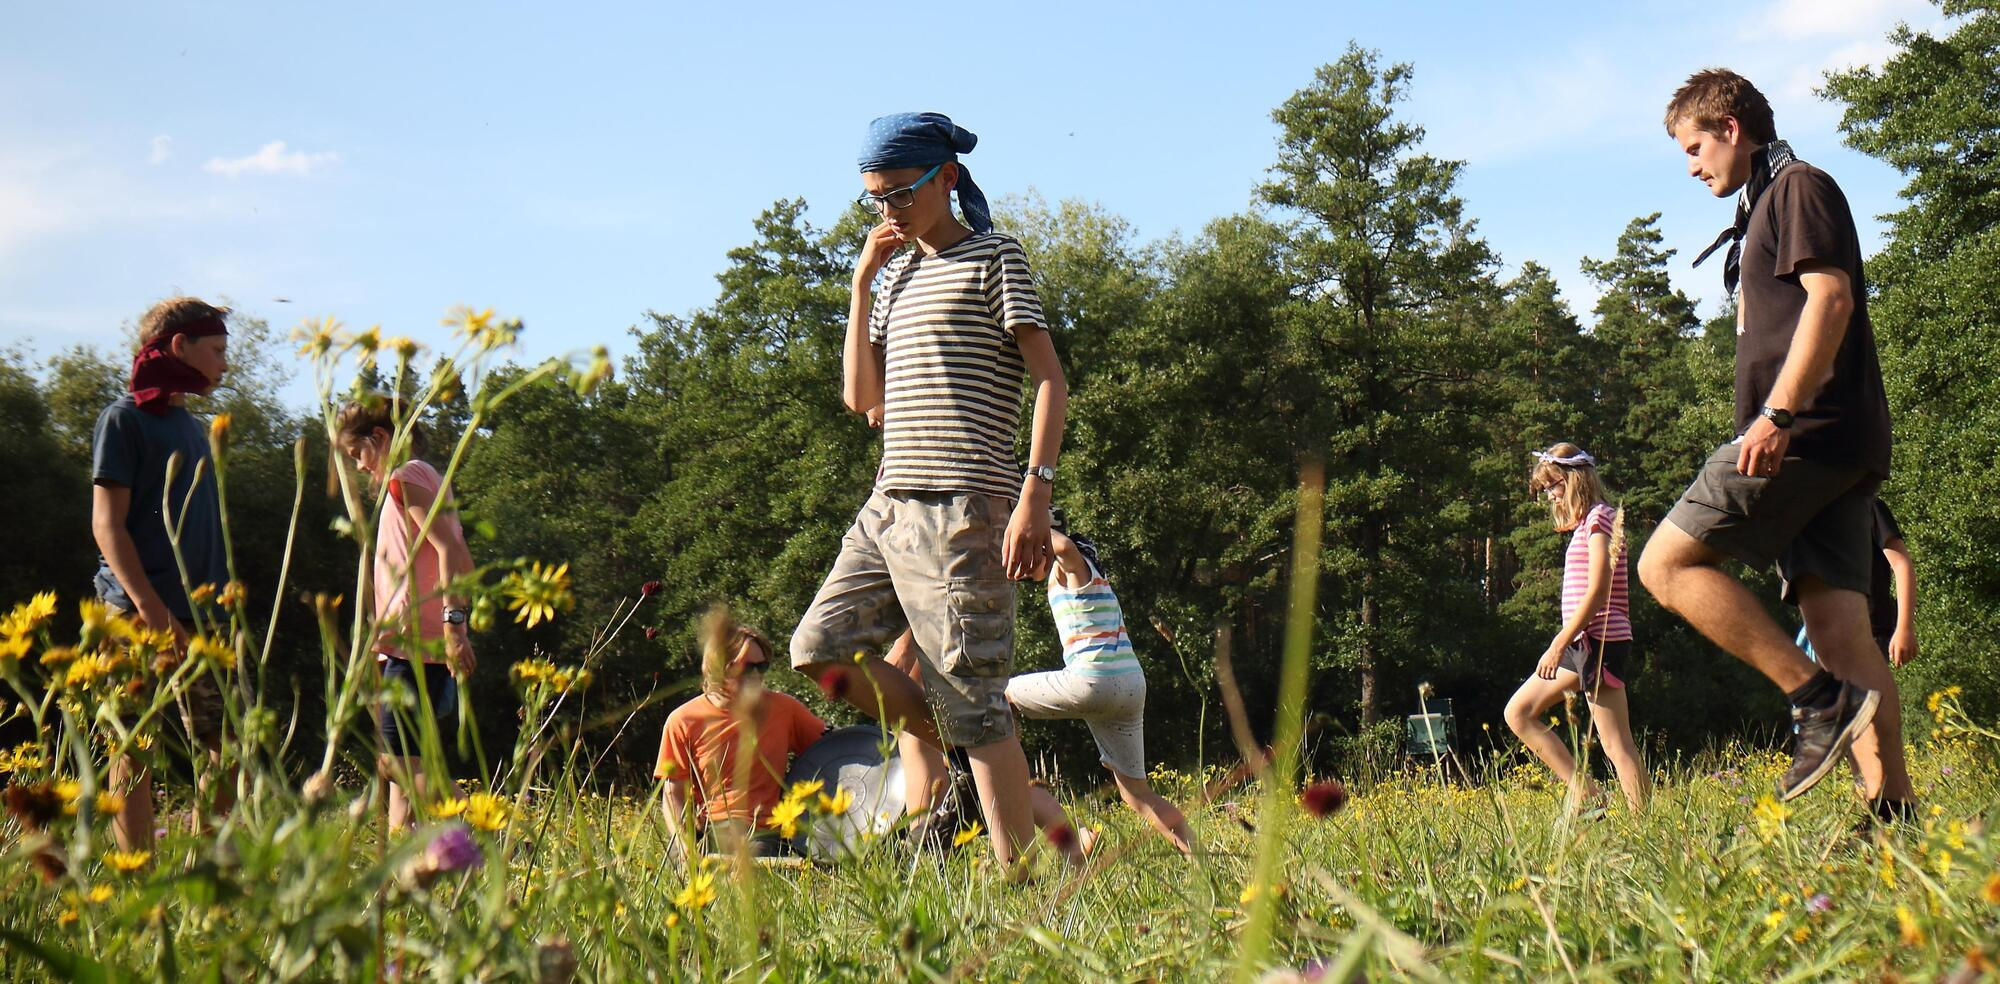
\includegraphics[width=12cm]{img/anpetu_tabor/hra.jpg}
\end{center}

% subsubsection honění_bizonů_a_buvolů (end)

\subsubsection{Cestování lodí} % (fold)
\label{ssub:cestování_lodí}

šli jsme do lesa a tam jsme vyděli několik lodí/udů udové měli šátky a běhali k jinému stromu na kterém byl papír třeba srí lanka a uďa který jel na srí lanku tak potřeboval peníze na suroviny a další věci a mi jsme mu mohli půjčit peníze a když na lanku doje se šátkem tak nám dal dvojnásobek nebo 3x nebo někdy 4x a ostatní co přispívali na lodě mohli někomu uďovi vzít šátek a jakmile uďa stratí šátek tak loď skrachuje a všechny peníze co jsme na loď vsadili propadli měli jsme každý 200 Kč a většina skončila cca u 1000 Kč

\podpis{Grizzly}
% subsubsection cestování_lodí (end)

\subsubsection{Bar} % (fold)
\label{ssub:bar}
setkali jsme se s Hanjetu u jídelny která byla zakrytá dekama a unit byli různý uďové/námořníci který se s námi o něco vsadili a když jsme vyhráli tak nám dali peníze a kdy jsme prohráli tak nám vzali peníze a za peníze jse si mohli koupit různý moc dobrý věci čokoládu, sušenky a další různý šladkosti nebo jsme si mohli vydělat peníze jinou cestou někdo někoho pocozí na dvojkoláku, namasíruje a tak dále

\podpis{Grizzly}
% subsubsection bar (end)

\subsubsection{Manévry} % (fold)
\label{ssub:manévry}

Nej dřív jsme šly k rybníku a tam se vibourala loď a potom sm šli do ostrovce a tam k rybníku kde byl papírek a od tam tud sme šli k dalšímu papírku, až jsme došli do nějaké vesnice, kde na nás čekali Vrtule a Humr. S nima jsme přespali mezi rybníkama Vosovice a Žabák. Ráno jsme vyrazili k rybníku Zhoř, kde jsme u stavidla našli papírek v morseovce.

Dál jsme šli do Nevězic přes nějakou vesnici, kde jsme měli počítat dřevěná zvířata. V Nevězicích jsme se naobědvali a pokračovali jsme k rozcestníku Luh. Od tamtuď jsme šli k rozcestníku Lipice, který byl asi 8 km od Luhu. Cestou jsme šli přes nějakou vesnici, kde nám jedna paní doplnila vodu a navíc nám dala i bonbóny. Potom jsme šli k mostu přes řeku, kde byli uďové a oznámení, že se zítra na hradě Zvíkov sejdou piráti, a že pokud chceme pomoct, že se máme ráno mezi 9:00 a 10:00. Tak jsme zamířili k lesu pobíž hradu, kde jsme se potkali se skupinkou Plejtváci a Borci. Ráno jsme šli na hrad, kde jsme potkali piráta Strniště jehož deník byly ty papírky, co jsme nacházeli.

Ten nám řekl místo, kde byla schovaná mapa (část) k pokladu Žaka Hnědovouse. Pak jsme se vraceli do tábora a byli jsme první!

\podpis{Anežka}
\begin{center}
	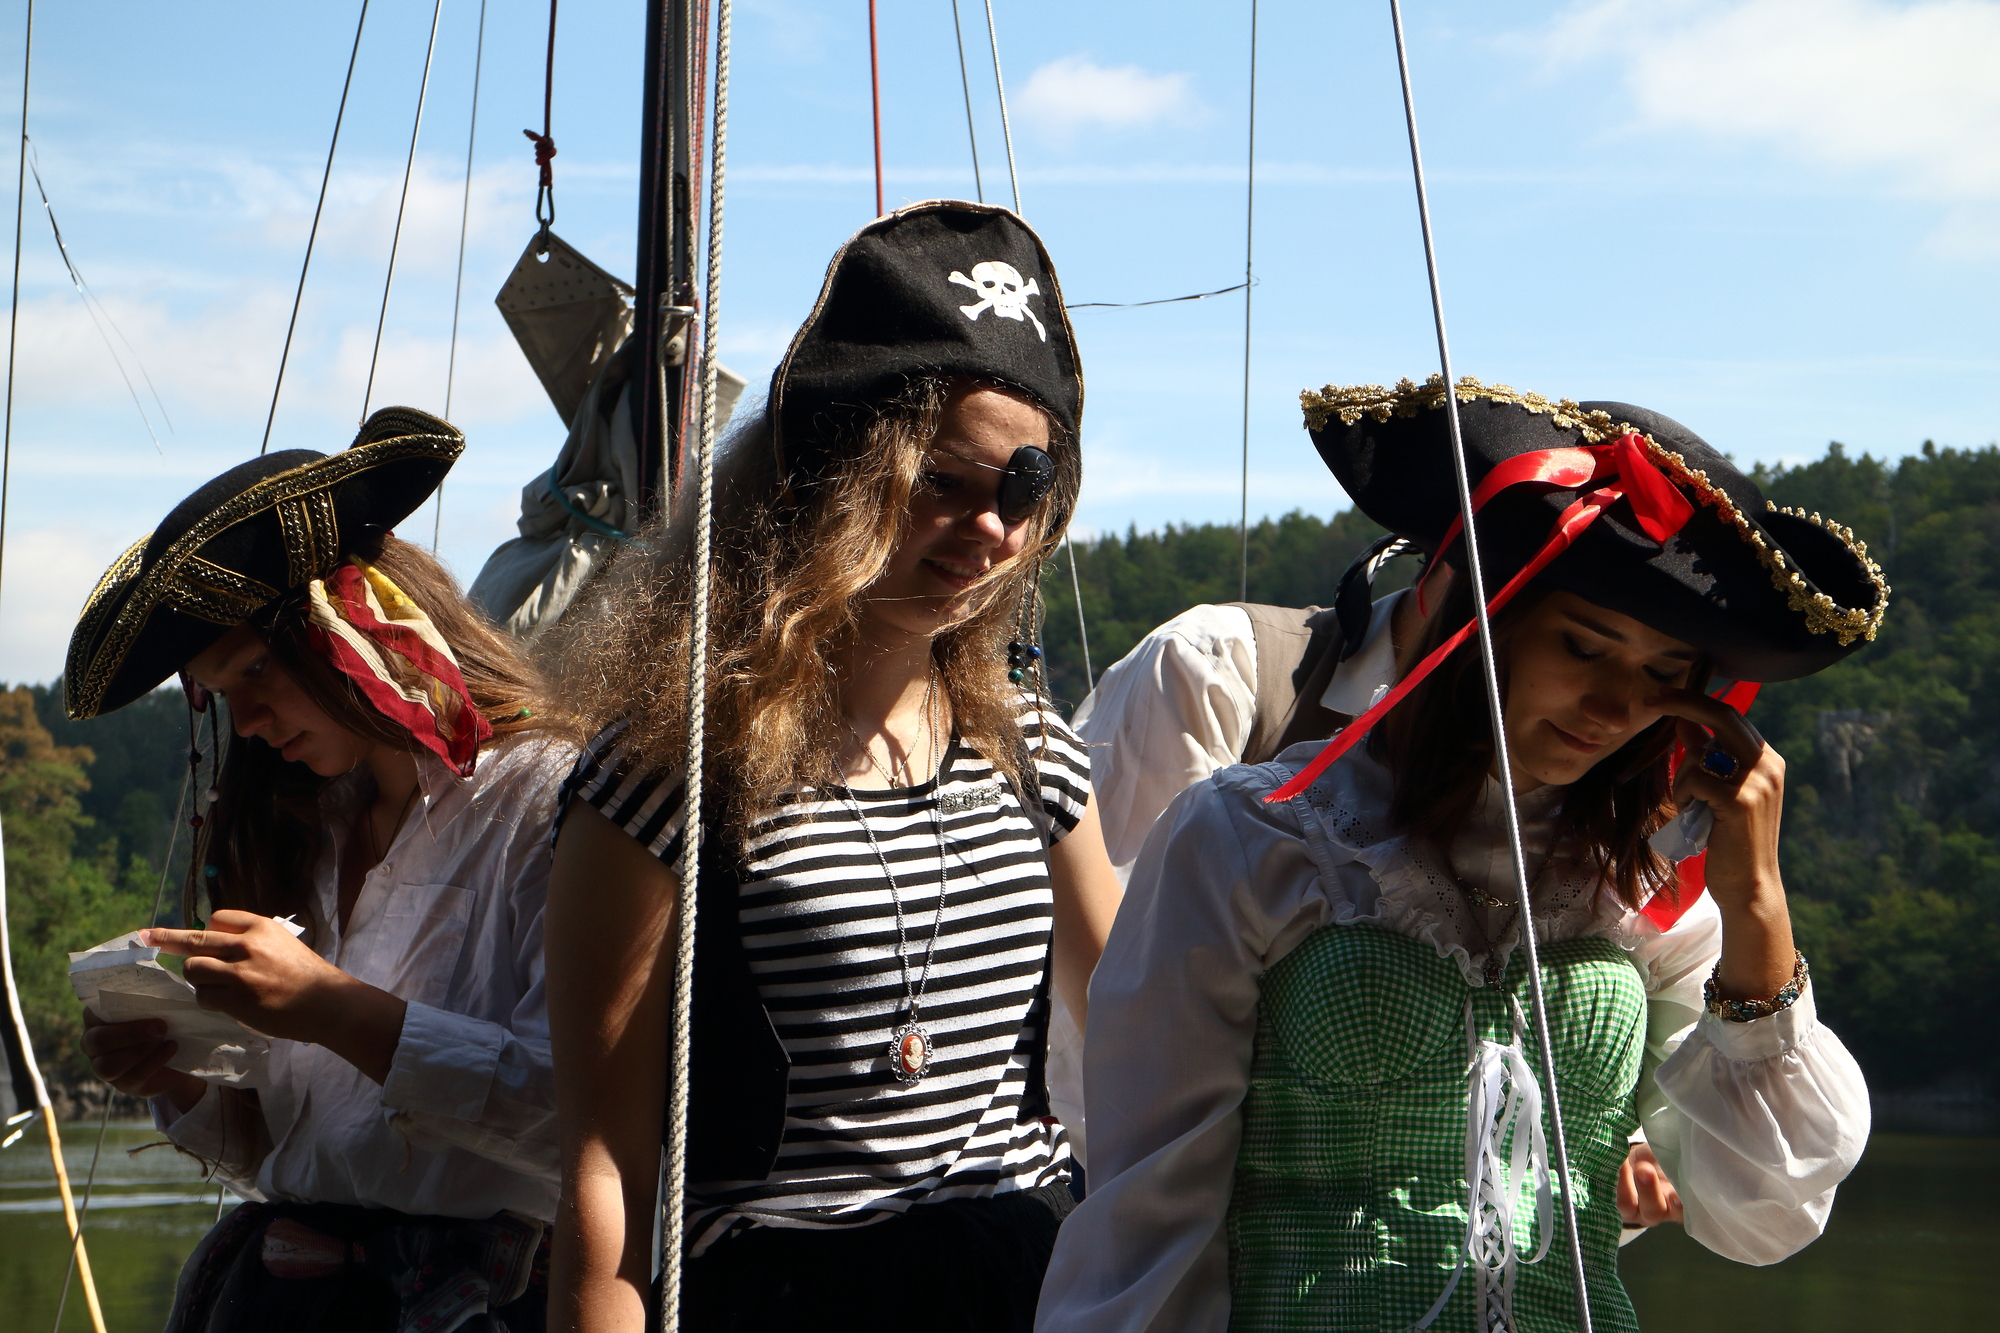
\includegraphics[width=8cm]{img/anpetu_tabor/pirati.JPG}
\end{center}

% subsubsection manévry (end)

\subsubsection{Etapková hra} % (fold)
\label{ssub:etapková_hra1}

Sice jsme získali mapu, jenže na ní není zakreslené místo, kde se nachází poklad.

Takže jsme měli na louce najít naše piráty a získat od nich tři indície, které pak spojily všechny skupinky dohromady a vyšly z toho „souřadnice“ pokladu.

\podpis{Anežka}


Nakonec jsme zjistili, že je to mapa NEPROBÁDANÝCH ÚZEMÍ.

\begin{center}
	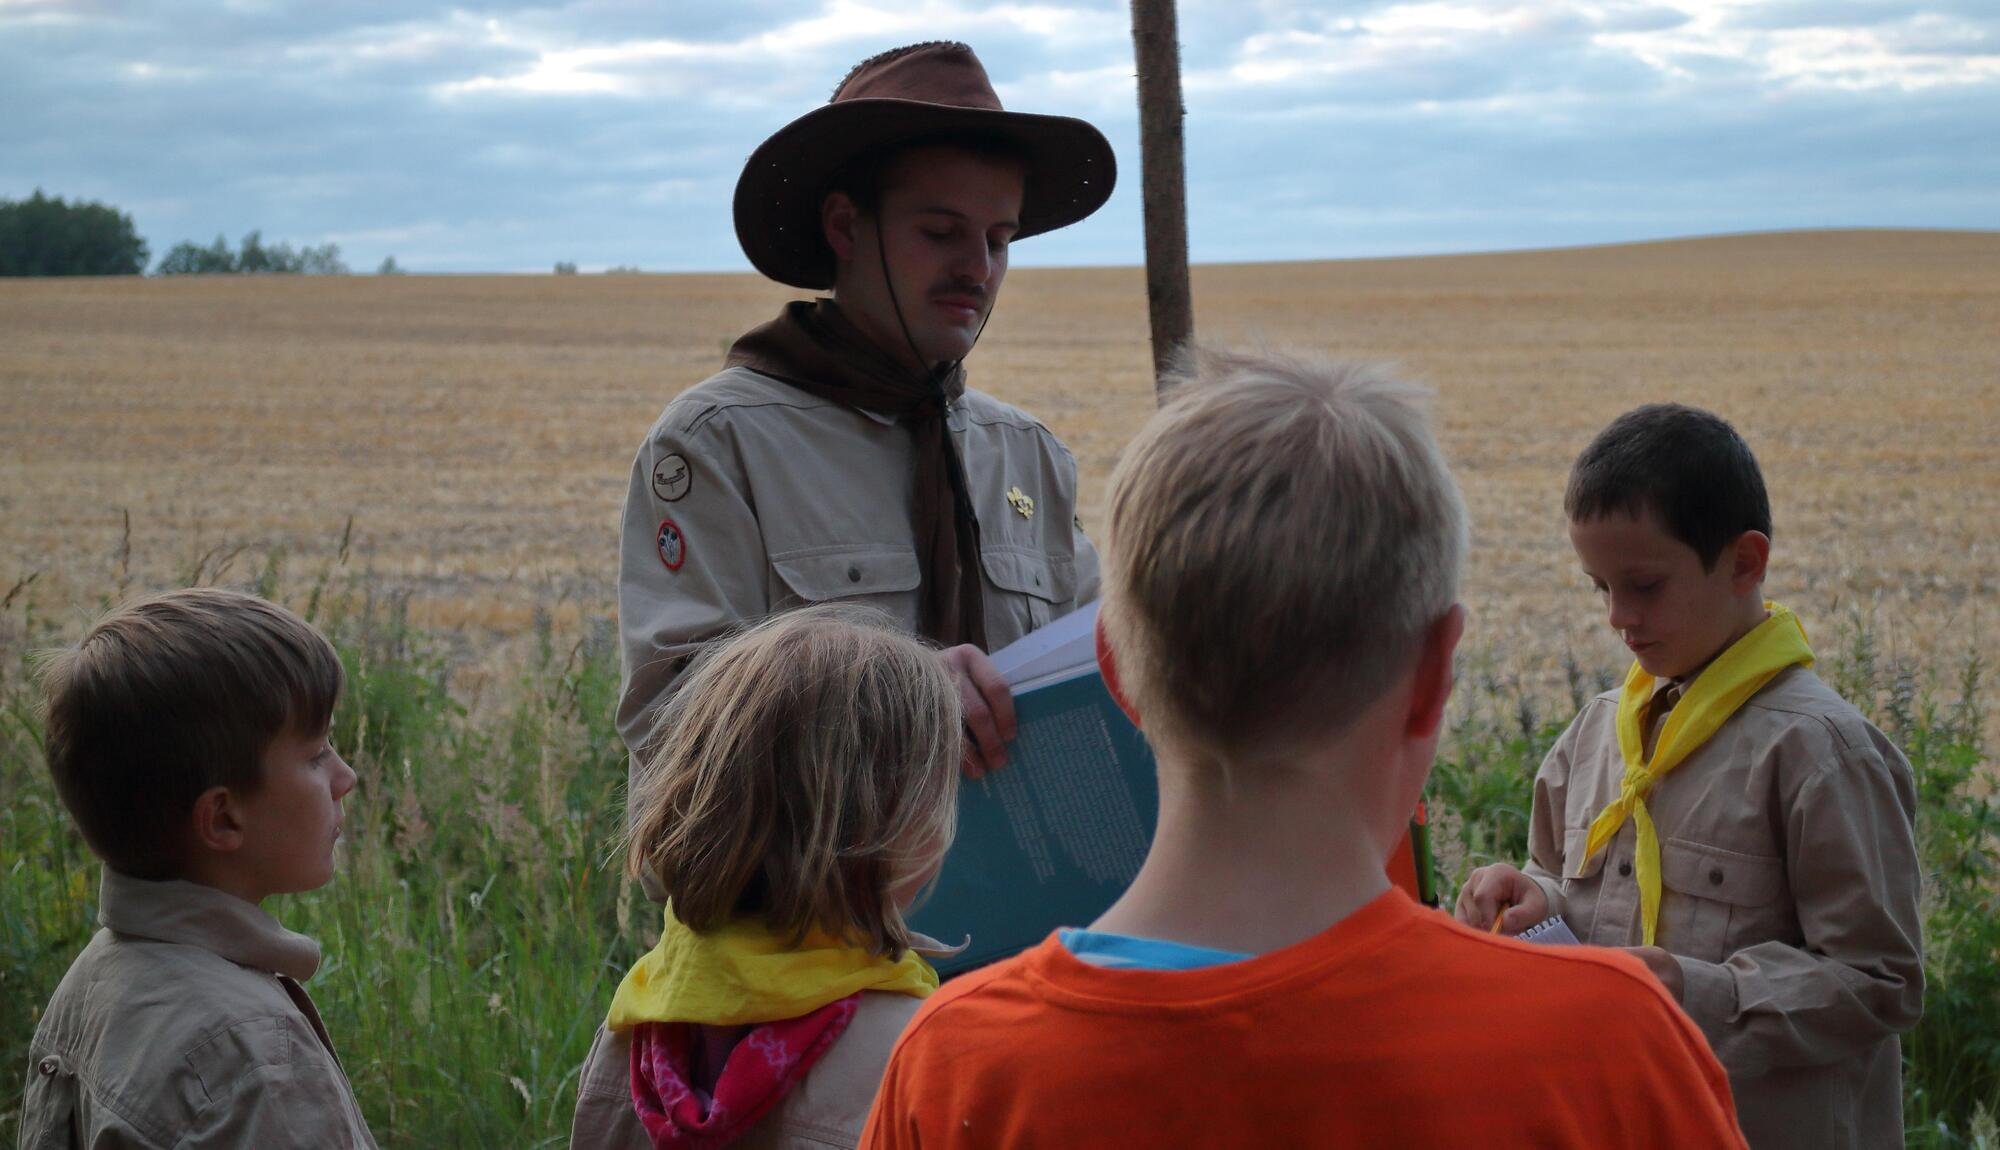
\includegraphics[width=10cm]{img/anpetu_tabor/svojsik.jpg}
\end{center}

% subsubsection etapková_hra (end)

\subsubsection{Etapková hra} % (fold)
\label{ssub:etapková_hra2}

kapitínce kukumbrii se stratil papoušek a dalších spousu věci tak jsme šli na viznačené místo kde ty věci jsou a mi jsme si museli nakreslit mapu abychom věděli kde ti věci jsou a mohli tam doplout našli jsme tam například, tužku, sprej, vlajku nebo něco takového. Když jsme měli všechno zapsáno (nelbo ono jsme na to měli určitý čas ta-takže jsme měli co jsme měli ale byl to dostateční čas) tak jsme pak šli do tábora

\podpis{GRIZZLY}
% subsubsection etapková_hra (end)

\subsubsection{Vařící etapka} % (fold)
\label{ssub:vařící_etapka}

Uďové nám oznámili, že máme uvařit pro Kukumbrii oběd, protože bude mít teď někdy narozeniny. Rozhodli jsme se, že budeme vařit v Borúwčím týpku, kam jsme si začali nosit suroviny na hodněchodový oběd pro Kukumbrii. Nakonec jsme měli: 1 rajče, skoro celou okurku, pytlík mouky, 7 brambor, 1 krajíc chleba, 5 vajíček, olej, sůl, koření, a hlavně rybu. Byla to ryba která měla hodně kostí, takže jsme měli takové maké kousíčky, které jsme smíchali s vajíčkem a moukou. Taky jsme se pokoušeli osmažit hranolky, ake nakonec jsme je rozmačkali na kaši, chutnaly tak líp. Taky jsme udělali jako přílohu chleba ve vajíčku. Kukumbrie řekla, že je to dobré.

\podpis{Anežka}
\begin{center}
	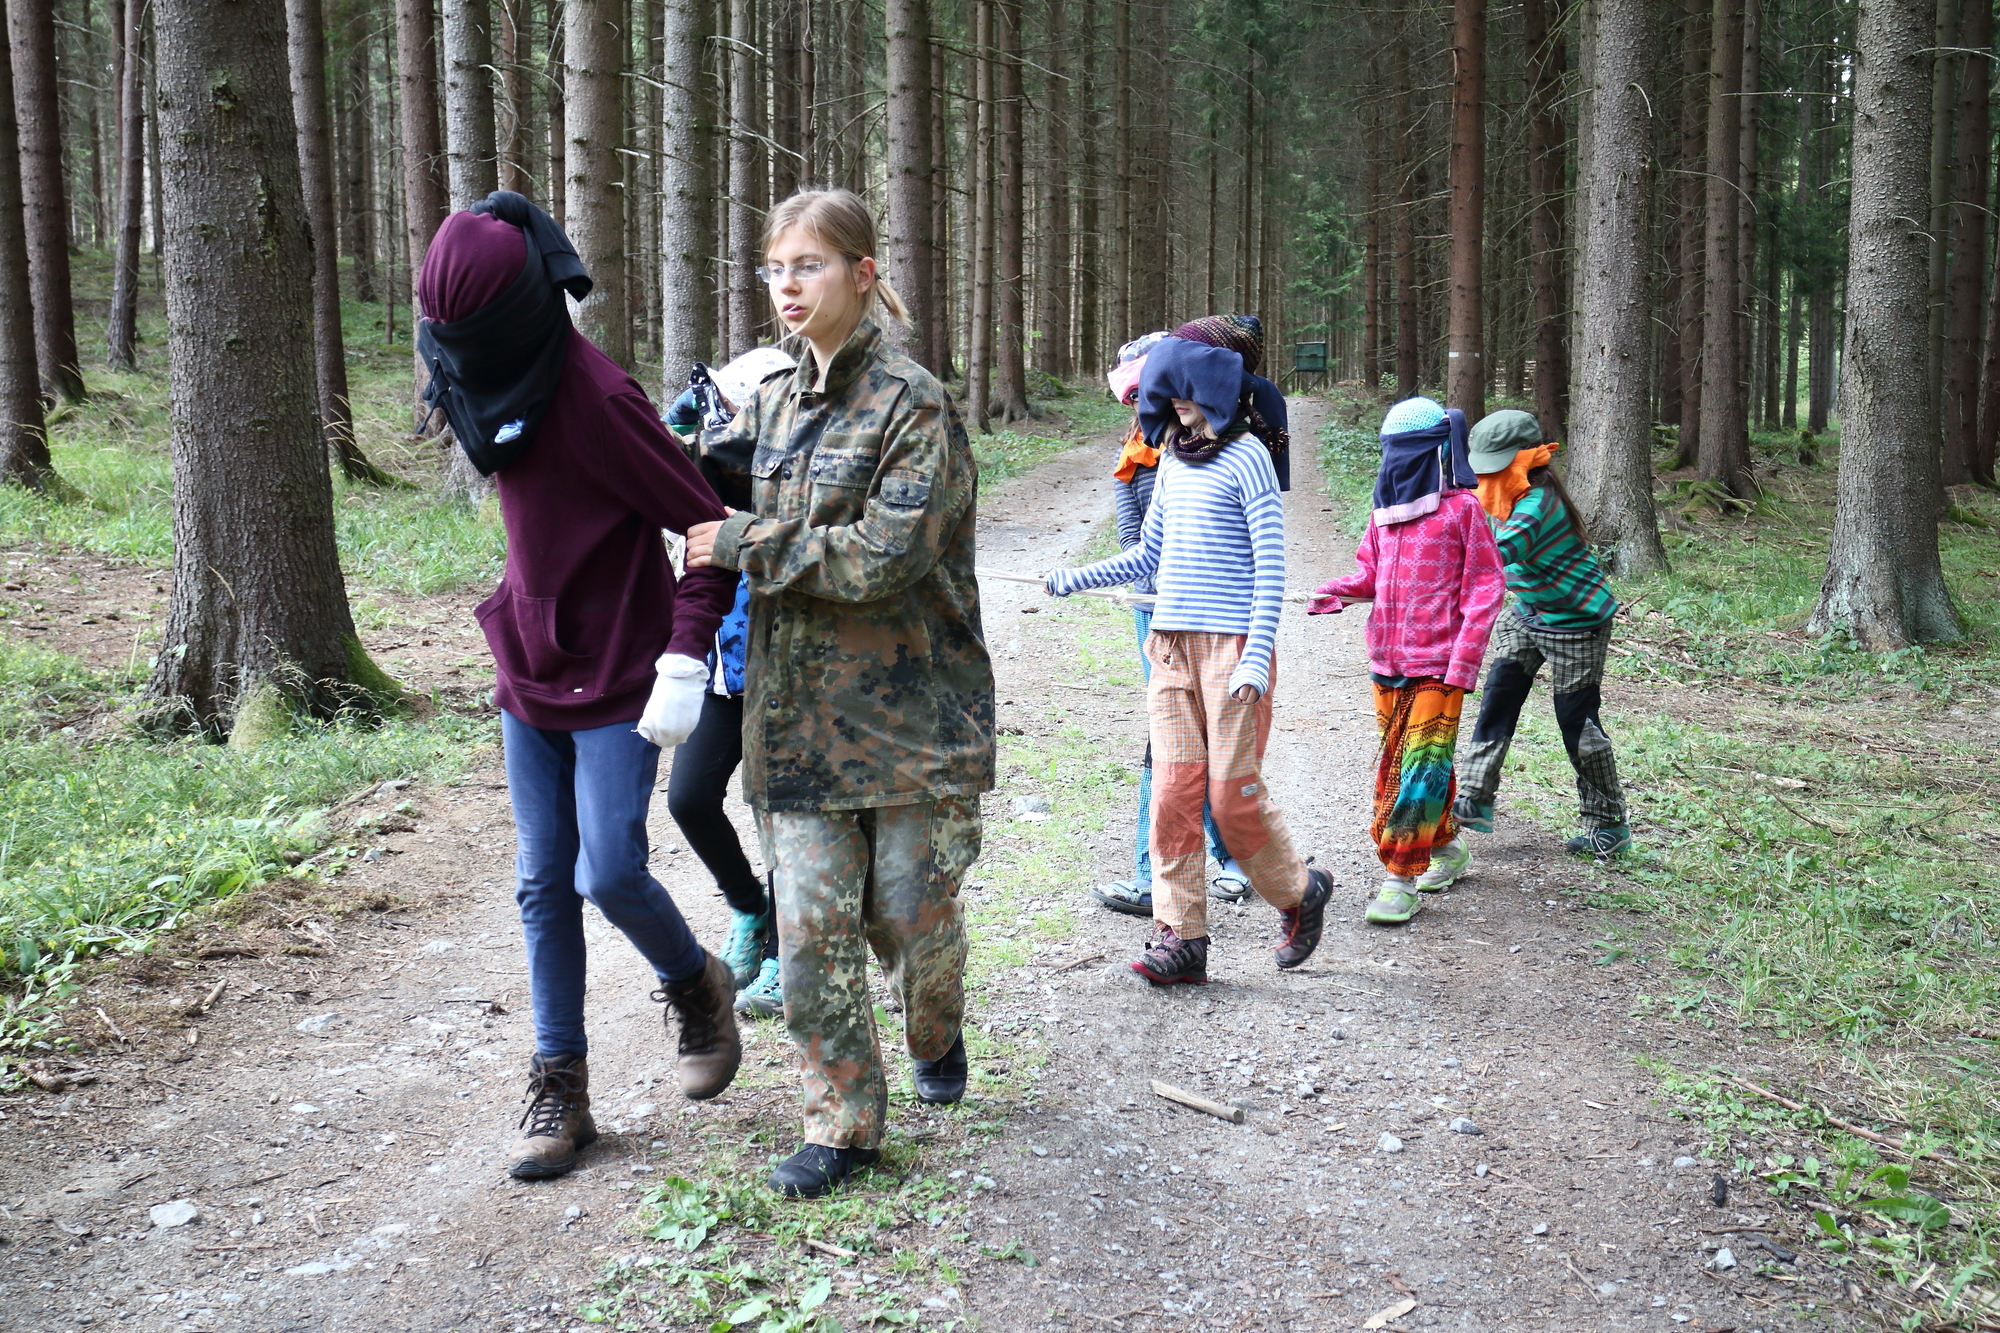
\includegraphics[width=8cm]{img/anpetu_tabor/vorvo.JPG}
\end{center}

% subsubsection vařící_etapka (end)
\subsubsection{Bar} % (fold)
\label{ssub:bar1}

kapitánka Kukumbrie měla narozeniny a tak musela být oslava dali jsme ji dárky: píšťalku, míček, tučňáka, čokoládu a bonbóny. pak byl bar jako takový: překecávaná, sirky, kolíčky a hlavně sladkosti a slavnosti.:-) Pak jsme šli ven protože jsme slišeli romantickou hudbu a tam byla kukuočko s Eulálií na lodi a bylo to jako v titaniku

\podpis{GRIZZLY}

% subsubsection bar (end)

\subsubsection{Vyvražďování} % (fold)
\label{ssub:vyvražďování}

kapitánka kukumbrie drsné oko měla mít narozeniny a protože je to skvělá kapitánka tak jsme prostě museli mít dárek a přáníčko tak jsme dostali seznam věcí co máme sehnat a vyrazili jsme abychom to stihli šli jsme do vesnice a tam jsme museli sehnat: nejoriginálnějsí vec k narozeninám, přáníčko a dort nebo jinou pochutinu (pak taky jsme měli sechnat ten dárek tak že si budeme vyměňovat mušličku) a do tábora jsme měli dojít nejpozději v 19:00 vše jsme stihli a dostali jsme spóóóusti věcí a dobrot:-)

\podpis{Grizzly}

\begin{center}
	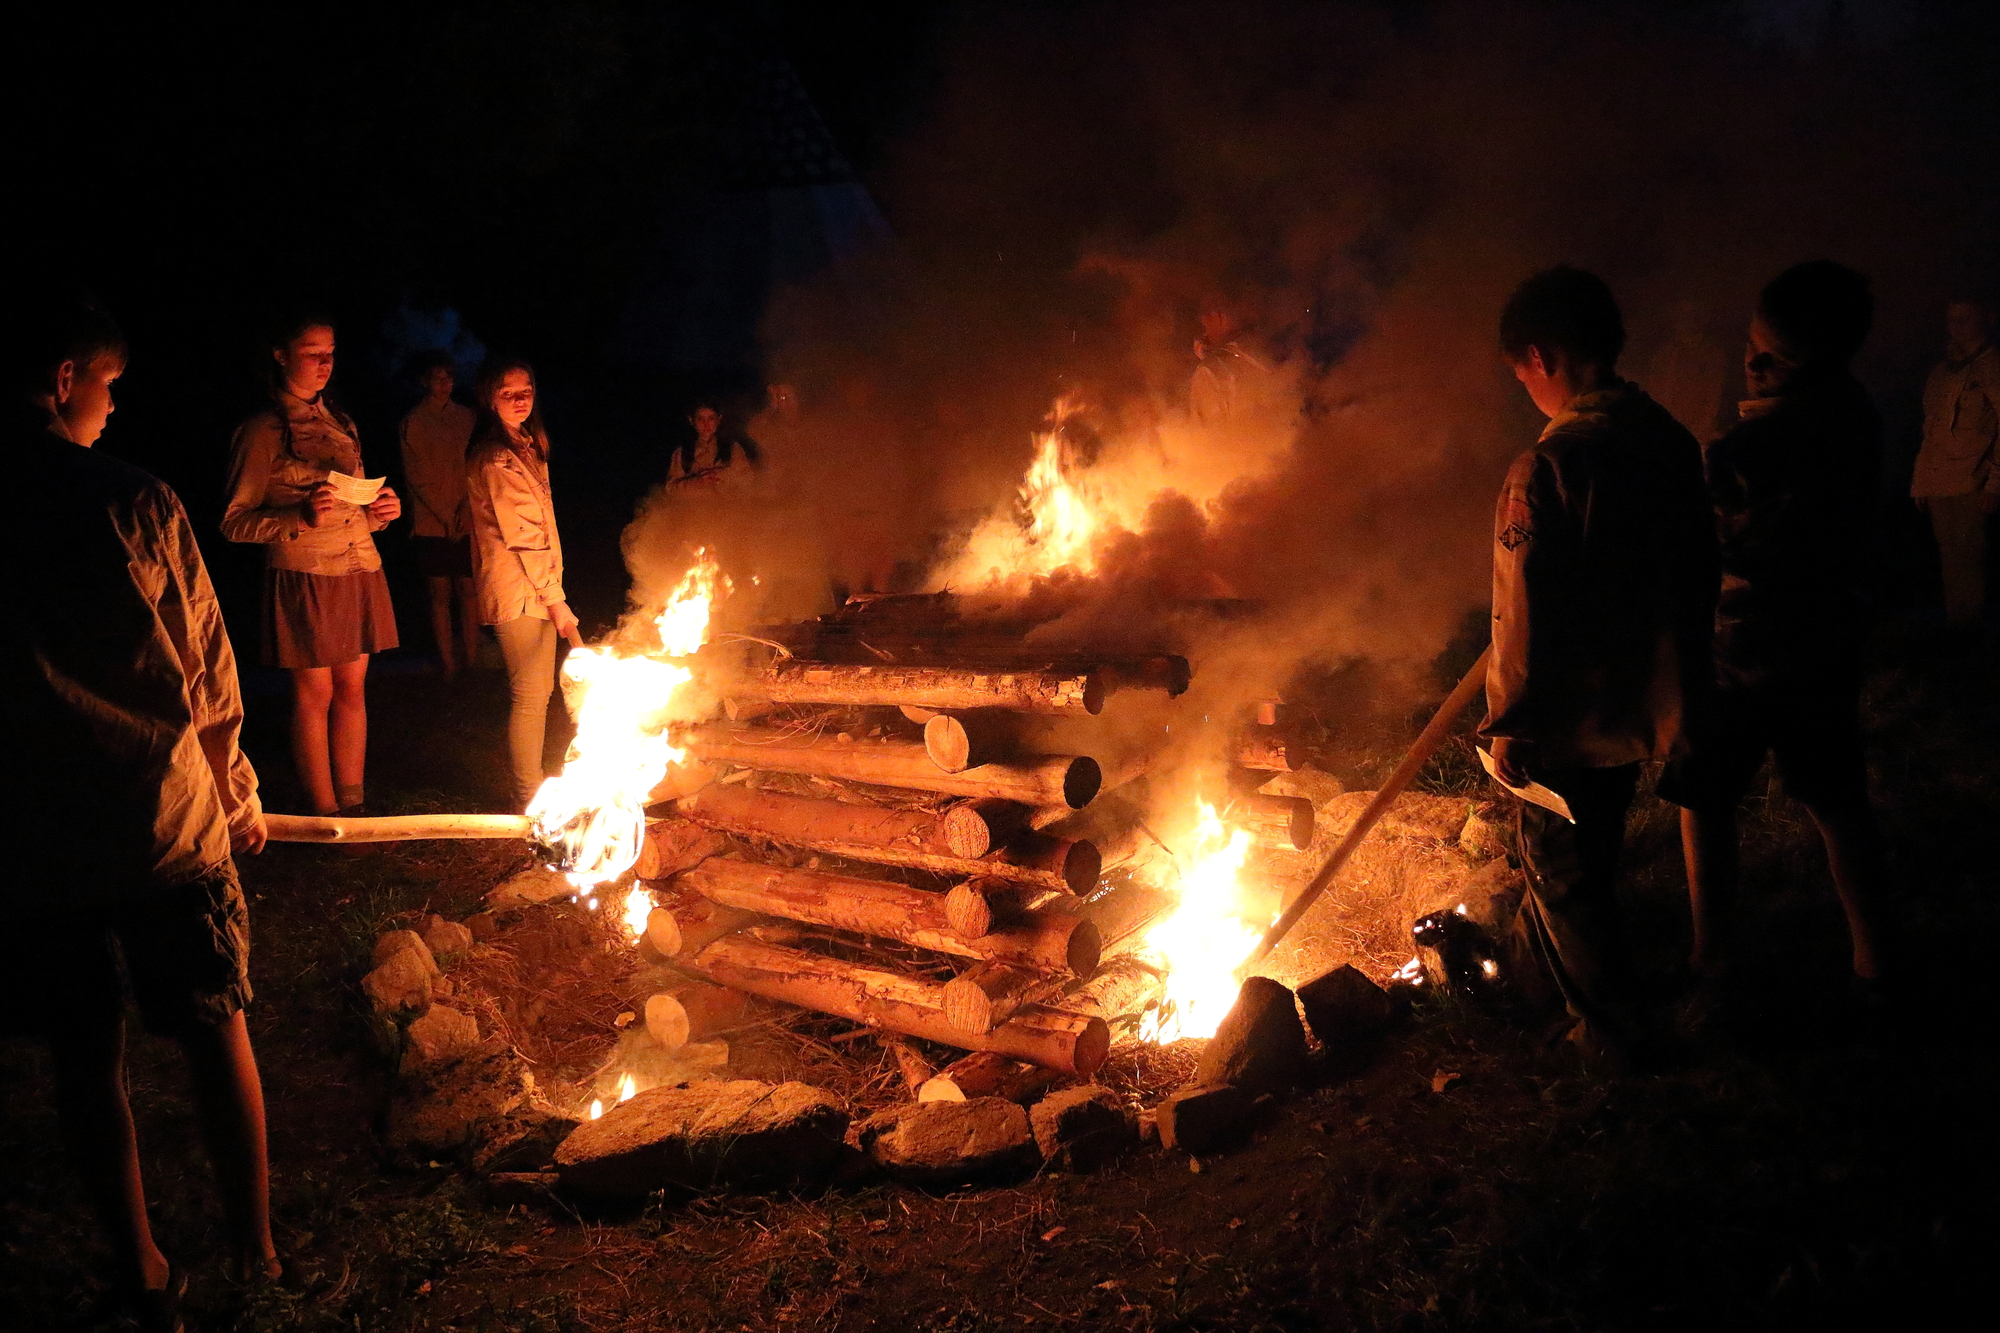
\includegraphics[width=12cm]{img/anpetu_tabor/taborak.JPG}
\end{center}

% subsubsection vyvražďování (end)
\subsubsection{Pokladovka} % (fold)
\label{ssub:pokladovka}

přepadli nás piráti a zabili kukumbrrii pak nás hned vyslali pomstít kukumbrii a najít poklad poslali nás do ostrovce na poštu kde vjsme měli najít čtiři obáli se jmény etapek v obálkách bylo napsáno v šivře ke je poklad (v šifrě) tak jsme tak došli a tam byla další správa o tom že si z nás vystřelili přesněji napsáno ha, ha napálili jste se hlupáci jen jsme získali čas na zakopání pokladu vraťe se do tábora Jonatán nám naštěstí řekl kde je poklas a museli jsme procházet tábořiště domorodců a pak jsme přešli rybník k ostrůvku kde byli piráti kteří po nás začali střílet naštěstí jsme mohli používat jejich papírové koule které používali jako střelbu a pomalu slábli a slábli až umřeli pak jsme našli místo kde by mohl být poklad a vykopali jsme ho tam bylo egzotické ovoce tak jsme ho vzali do tábora kde byla supr hostina: řízky, okurky, papryky, rajčátka a tak dále a protože jsme přijeli hodně pozdě tak jsme zalezli do sPacáčků a spali Grizzly a Karkulka


% subsubsection pokladovka (end)
% chapter lodní_deník_etapkové_skupiny_černí_rytíři_anpetu_ (end)

\begin{center}
	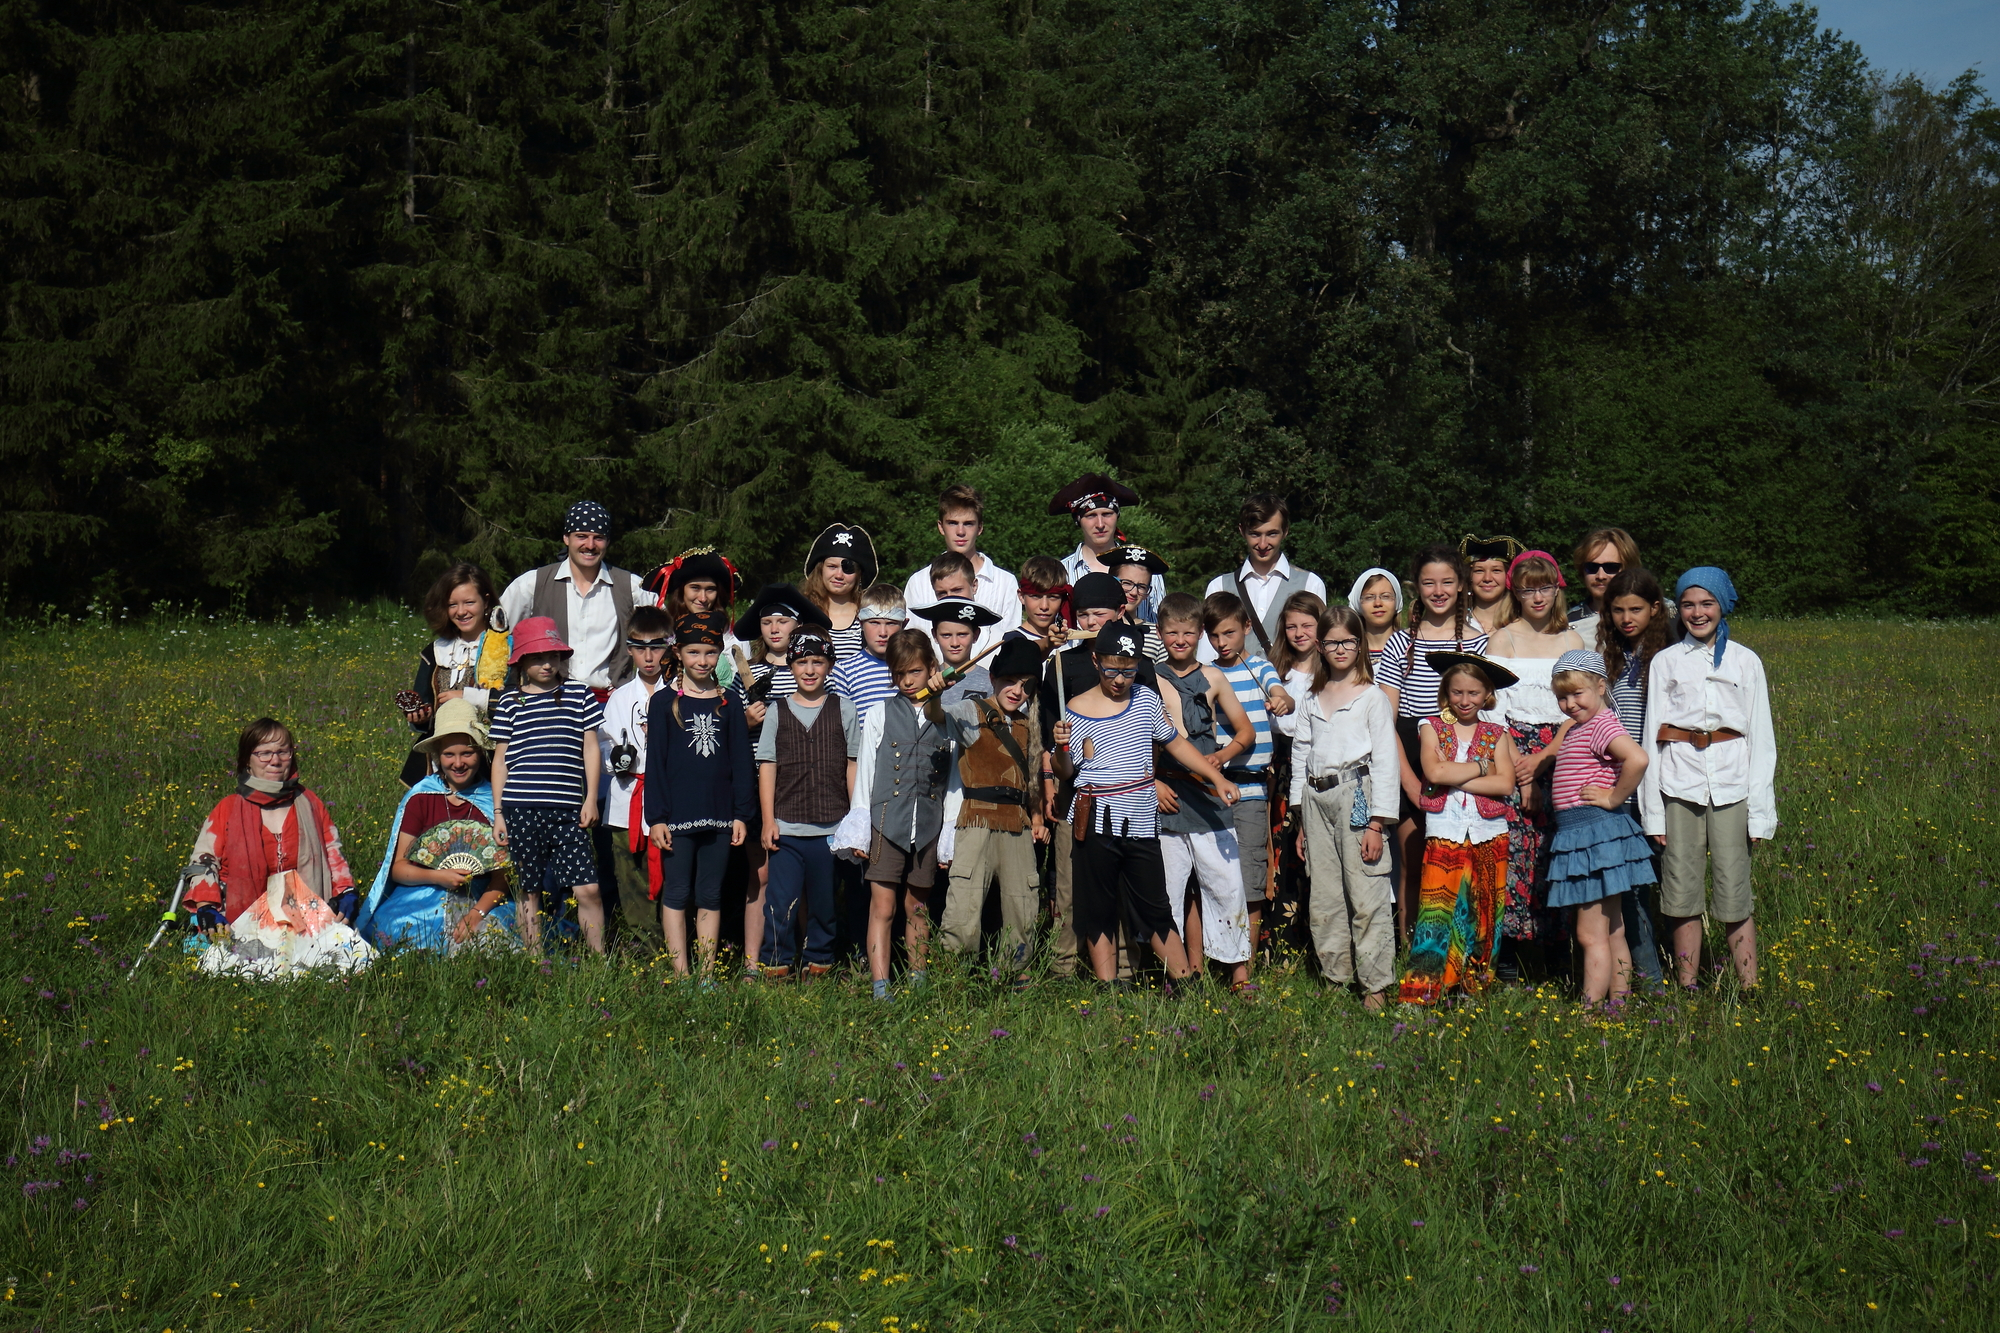
\includegraphics[width=\textwidth]{img/anpetu_tabor/spolecna.JPG}
\end{center}
\clearpage

\chapter{Střípky očima účastníků} % (fold)
\label{cha:střípky_očima_účastníků}

\subsection*{Kompoti} % (fold)
\label{sub:kompoti}


\begin{multicols}{2}


MANÉVRY BYLI DRUHÝ TÝDEN OD PONDĚLÍ DO STŘEDY. DRUHÝ DEN V ÚTERÝ JSEM ZNIČIL MAPU DÍKY VODĚ. A NA VYVRAŽĎOVÁNÍ MAPU ZNIČILA KARKULKA. NA DRUHÉM TÁBORÁKU JSME SE STRAŠNĚ SMÁLI, PROTOŽE KUŘE CHTĚL ZBALIT KARKULKU ( Z POHÁDKY) A TU HRÁL ŠERIF. A POSLEDNÍ DEN JSME VZALI 5 KILOVOU PALICI A NIČILI JSME POSTELE A ZASIPÁVALI OHNIŠTĚ A PAK JSME ODJELI.


\podpis{Ledoborec}


JEDEN DEN JSME PO OBĚDĚ JSME KAŽDÁ DRUŽIINKA MĚLA SVŮJ PROGRAM. NAŽE DRUŽINKA MĚLA "KOPÁNÍ SVÉHO HROBU,,
JÁ ŽEM SI KOPAL ÚNIKOVOU CESTU ALE PRÁSKLI MĚ, TAK JSEM MUSEL NAJÍT JINOU SESTU ALE NÉŮSPĚČNĚ TAK JSEM SKOUŠEL ASI PŮL HODINY A PAK JSME SKUSIL POPLAZIT POD KLÁDOU A NYKDO SI MĚ NEVŠIM. UTÍKAL JSEM PO USCHLÝM POTUKU A KDYŽ JSEM PŘEŠKOČIL KLÁDU A PODOM A PODOM JSEM ZAPAD DO PAHNA. VYHRAPAL JSEM SE A PODOM JSEM ŠEL PO PEVNINE A TAM MĚ CHYTIL HUMR.


\podpis{Mýchačka}


DNY 8.11. AŽ 10.11. JSME BYLI NA TROJDENCE VE VOLYNI. DRUHÝ DEN JSME VLAKEM JELI NA STANICI \\,,KUBOVA HUŤ." PAK JSME ŠLI NA ROZHLEDNU ,, BOUBÍN", KDE NÁM SNĚŽILO A BYL TAM KRÁSNÝ VÝHLED. VŠUDE NA ROZHLEDNĚ BYLI OMRZLINY. CESTOU NA ROZHLEDNU JSEM VÁLEL KOULI ZE SNĚHU, ALE BOHUŽEL MI CESTOU SPADLA. KDYŽ JSME SE VRÁTILI DO KLUBOVNY, TAK JSEM BOHUŽEL OSTATNÍ NAUČIL POUŽÍVAT HLÁŠKU, KTEROU NÁM VEDOUCÍ ZAKÁZALI POUŽÍVAT. CESTA ZPĚT NÁM TRVALA 1hod. A 30min. TROJDENKU JSEM SI MIC UŽIL.


PS: TA HLÁŠKA BYLA ,,KUR VAJÍČKA SNÁŠÍ"


\podpis{Topík}



Trojdenka ve Vrchotových Janovycích
Nepamatuju si fakt nic z příjezdu “iajá javla!”[a] 
Ale pamatuju si . nic a Bla bla bla bla. No asi máte pravdu TOTO nebyla dobře napsaná. Tak teť opravdu začínáme. Takže Ořezával jsme klacíky ale byli krátké (javla[b]) A také jsme pařili benk ale ani jednou jsem nevyhrál javla[c],škoda alespoň jsem si zapařil pak sme jeli domů


\podpis{Poslední}


\columnbreak

TÁBOR
DOBRÝ BYLI MANÉVRY protože to bylo super ale dřely mě ramena protože jsem neměl mikynu.Taky byla super hlídka,jednou jsem vstal protož tu bylo asi 12 přepadlíku a jako jediný z Kompotů a honil jsem přepadlíky chytily jsme všechny a uvárali jsme je na provazy pak jsem šel snát. Super byli volné chvíle na psaní dopisů.


\podpis{Sumec} [d]


NEJHORŠÍ HLÍDKA:
BYL JSEM V KUCHINI SLYŠEL KORKY NAPŘED JSEM SI MYSLEL ŽE TOJE PŘEPAD ALE NEBYL TO PŘEPAD BYLO TO ZVÍŘE BYLATO NEZJISTIL JSEM TO


\podpis{Buffon} [e]

\columnbreak

NA TÁBOŘE BYLA ZÁBAVA MĚLI JSME 3x OHNĚ U 3. OHNĚ SEM SLIBOVAL BYLO T HUSTÝ. STAVĚNÍ TÍPÍ, VOLNÉ POLEDŇÁKY, JÍDLO, POSTELE (VIRÁBĚNÍ), ŠÍLENĚ MOC HER, OHNĚ VTEE PEE, A NÁVŠTĚVÁK, PROSTĚ DOBRÝ !!!
D

\podpis{ONRA.F}[f]\\ \vspace{5pt}
%\columnbreak


\subsubsection{Redakční poznámky:} % (fold)
\label{ssub:pozn}

% subsubsection redakční_poznámky_ (end)



{[a]}(napsáno šifrou polský kříž, když vynecháme v kódu písmeno ch dostaneme se k “jaká kauma”, tedy jaká karma, což jsme klukům zakázali a někdo si to oddřepuje poz. Alvise) \\
{[b]} opět polský kříž \\
{[c]} -||- \\
{[d]} Polský kříž \\
{[e]} obráceně než zbytek textu \\
{[f]} "Dřepí", poz. Alvise \\



\end{multicols}

\begin{center}
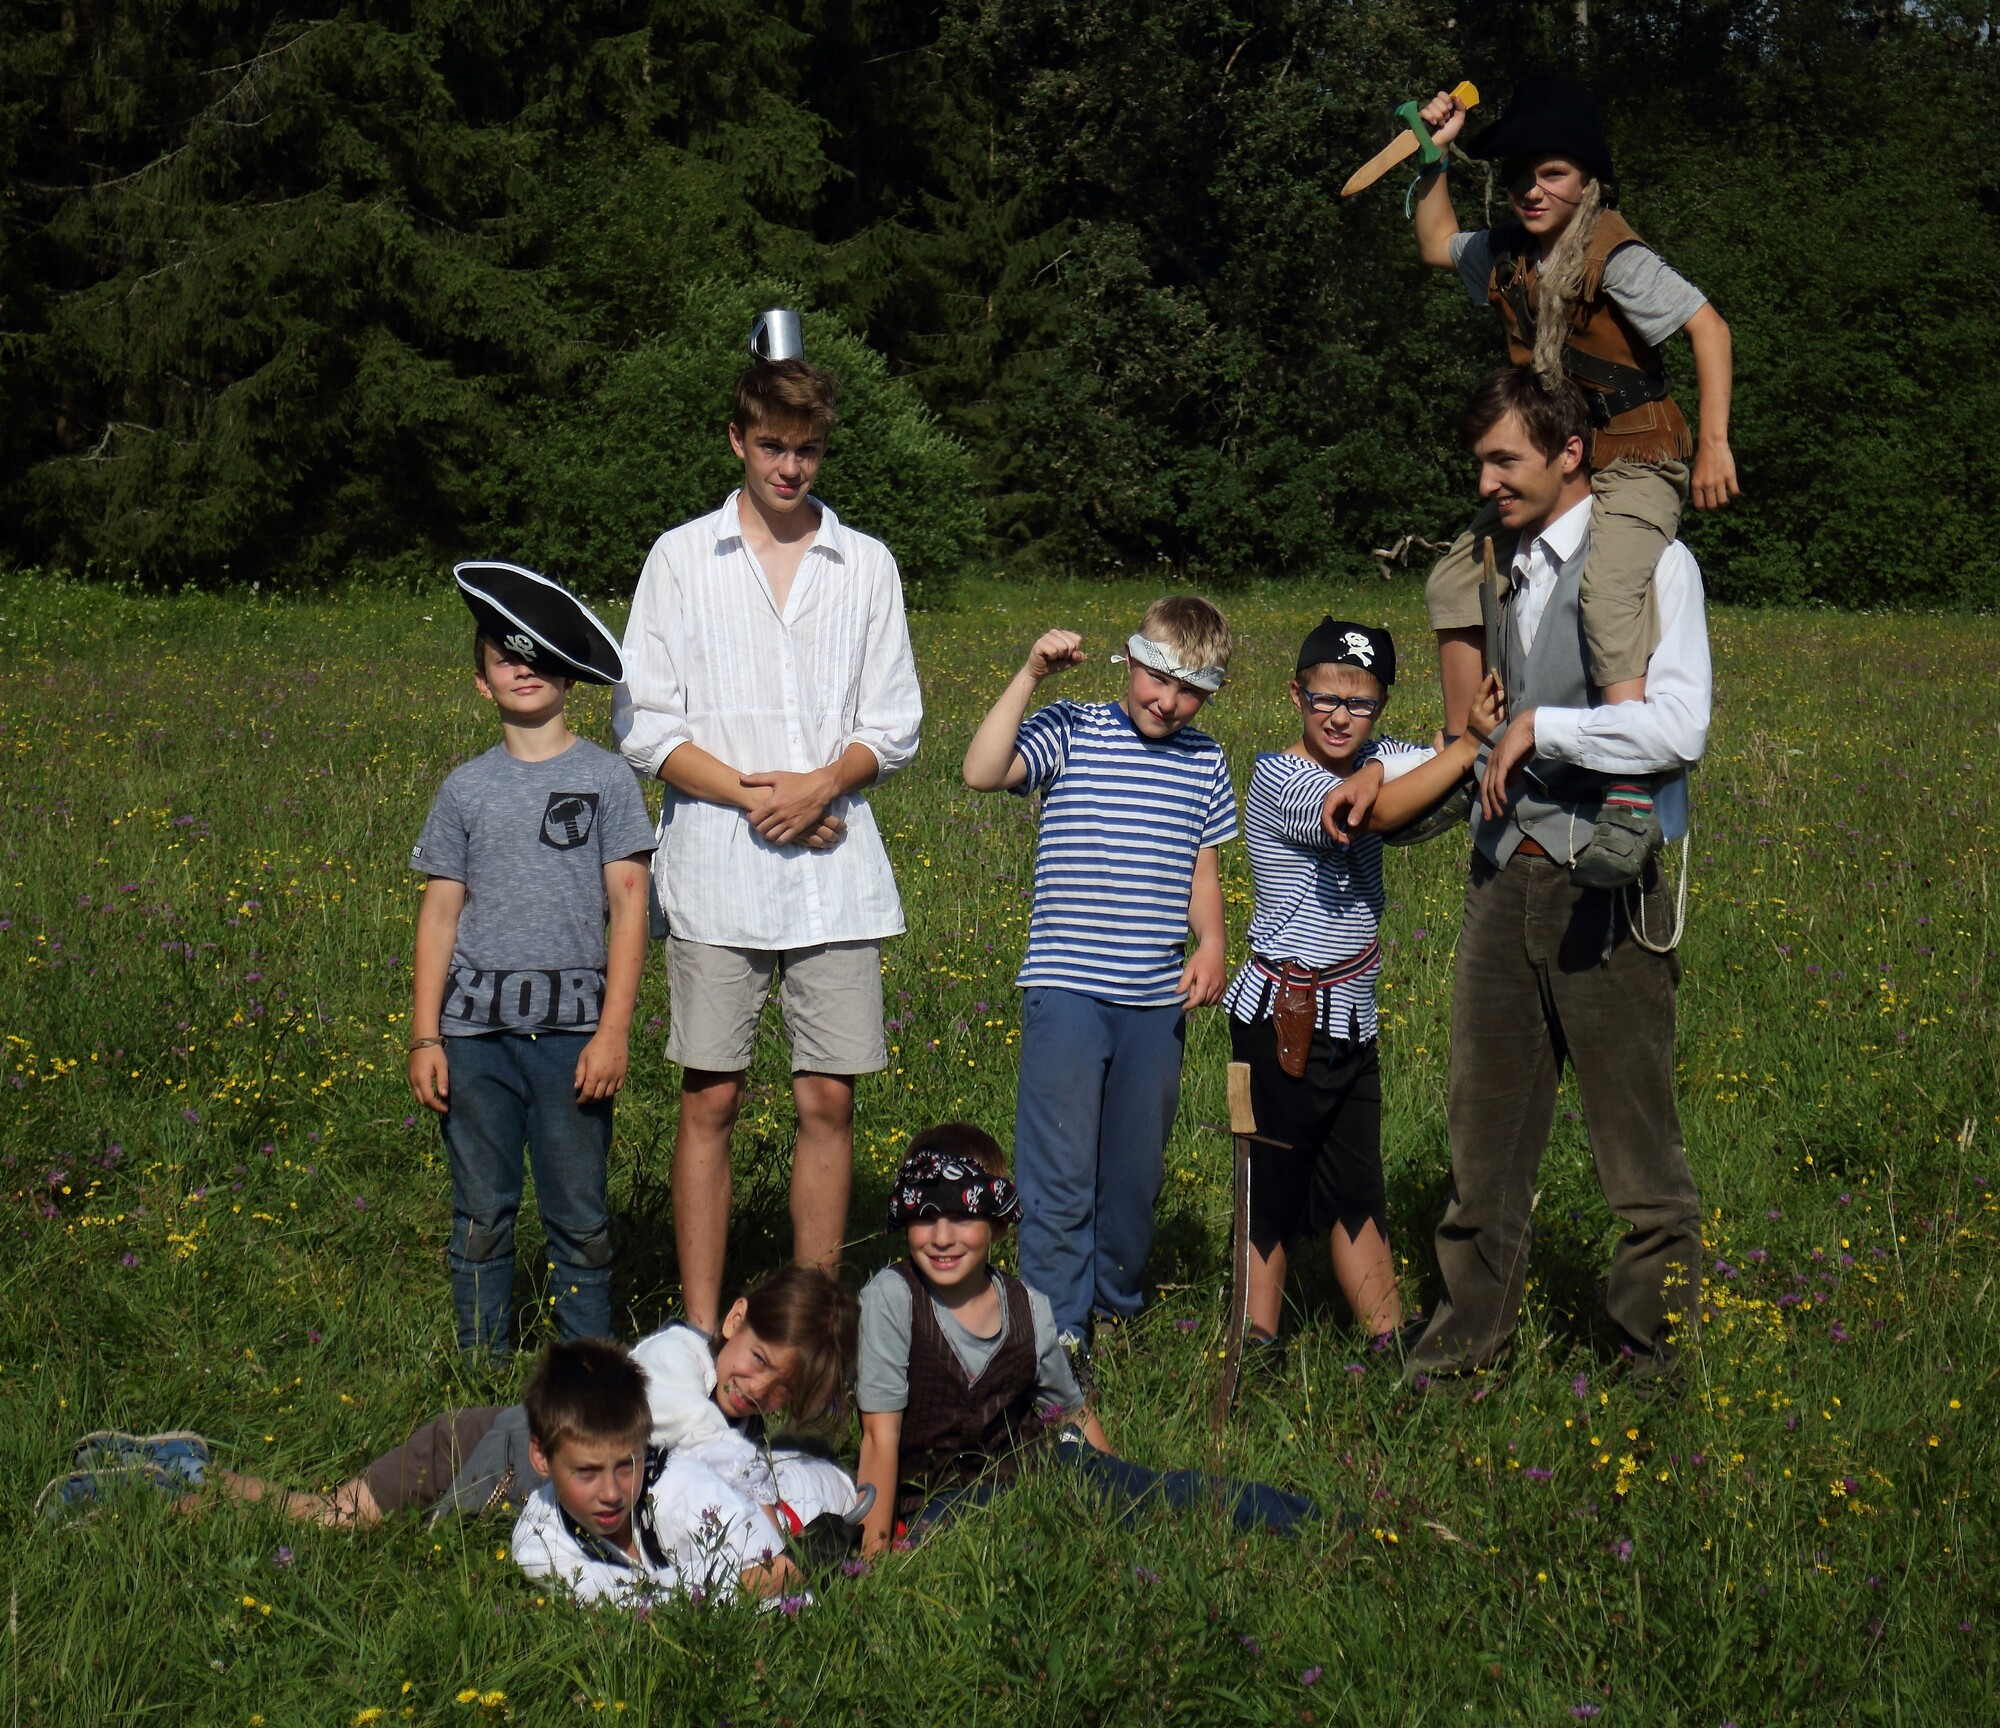
\includegraphics[width=9cm]{img/druziny/kompoti.JPG}
\end{center}

\clearpage
% subsection kompoti (end)
\subsection*{Eskymáci} % (fold)
\label{sub:eskymáci}

\begin{multicols}{2}
	

STRAŠIDELNÁ HLÍDKA

Když jsem měla hlídku tak se ozvalo VÁŽENÍ CESTUJÍCÍ VLAK PŘIJEDE NA DRUHOU KOLEJ.

\podpis{Zub}


NA TÁBOŘE!

Jednoho dne když Kujonka a Karkulka plnili úkoli a Kujonka mlčela a karKůlka bila slepá tak si pomáhali no chápete? tak jsem jim musela pomoct já Undži
Na táboře jednoho večera sem vodešla za Kujonkou z baru ven do polotmi, Kujonka tam dělala náramky potom jsme si povídali a povídali, až najednou zničeho nic spadl obří těžký strom! Kujonka vám to může potvrdit podpisem: Kujónka

\podpis{Undži}


Nejstrašidelnější a zároveň i nejvtipnější když jsem byla na hlídce a měla jsem přepad KDE mě svalili na zem a zacpali mi pusu (dva) pak když vylezla Debat bez ponožek tak na ní šel jeden a ostatní pohazovali věci jako zprej na latry, vložky, mouku a ostatní dohromady jich bylo asi osum.

\podpis{GRIZZLY}


Na pokladovce když ještě byli všechny skupinky spolu sme se honili a kujónce se namočil šátek do marmelády. kujónka  byla nešťastná a to hodně moc a moc. všichni jsme se snažili aby nebyla smutná ale najednou se jumbo podívala na ten šátek a řekla: “kujonko, vždyť to je undžin šátek.” Všichni jsme se smáli a pak se zjistilo že kujončin šátek mám já a že ten můj leží v táboře na undží posteli takže nakonec měla špinaví šátek undži a já ho na pokladovce neměla.:)

\podpis{KARKULKA}


Na táboře byl můj nejlepší zážitek, když jsem slibovala. Můj druhý nejlepší zážitek, byly to přípravy na slib po lese byli rozmístěny svíčky s otázkami když jsem je všechny vyplnila tak jsem šla za Pískletem s otom popvídat

\podpis{Čudlík}


NEJFTIPNĚJŠÍ: KDYŽ JSEM NAPODOBOVALA SLEPICI a PÍSKLE NEČEKANĚ DALA PODEMNĚ VAJÍČKO KDYŽ JSEM UKAZOVALA JAK biSEM VISEDÁVALA VEJCE 


\podpis{KUJÓNKA}


Na pětidence jsme se večer plížili za drakem protože jsme ho chtěli zapíchnout a drak říkal: já mám hlad druhá hlavo já mám taky hlad první hlavo to bude asi tím, že máme stejný žaludek.


\podpis{gingo}

\end{multicols}

\begin{center}
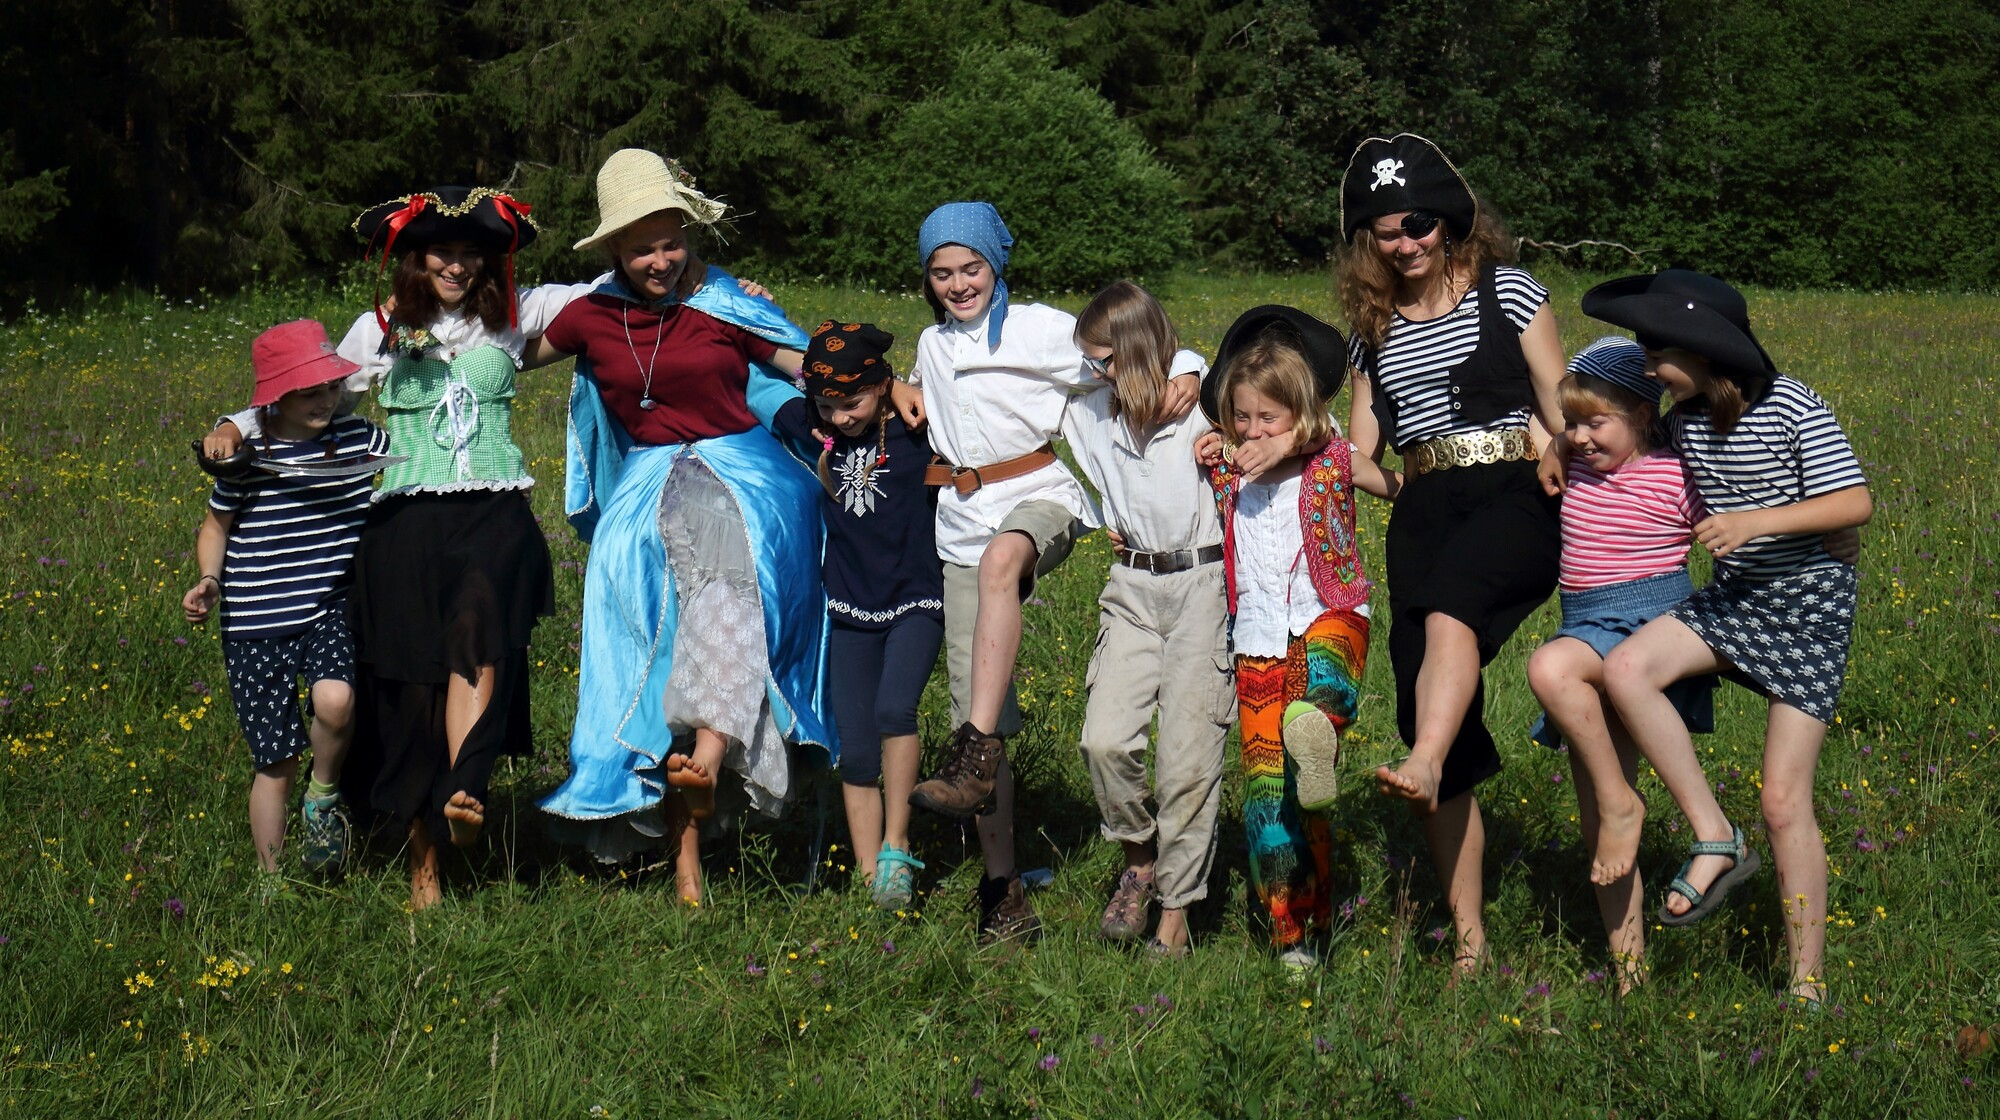
\includegraphics[width=12cm]{img/druziny/eskymaci.JPG}
\end{center}

% subsection eskymáci (end)

\subsection*{Urzoni} % (fold)
\label{sub:urzoni}

\begin{multicols}{2}
	
Noční hra
V noci nás vzbudili křikem, že loď hoří. Museli jsme běhat s hrnečkem pro vodu a hasit ohně v lese. U ohně ale byli piráti a chytali nás. Potom, co jsme ohně uhasili, jsme si museli odnést svoji věc z celty, která byla za ohněma. Noční hra se mi moc líbyla.

\podpis{Čertisko}

JEDNOU JSME SE RÁNO PODÍVALI NA PROGRAM. A TAM ODCHOD NA MANÉVRY URZONI: HAHAHA ODCHOD NA MAÉVRY TO URČITĚ NEBUDEME ODCHÁZET NA MANÉVRY. BORŮVKY: ZABALÍME SE POTŘEBUJEME SPACÁK, KARIMATKU…

\podpis{SNĚH.}

Na posledním táboře jsem nebyl a to mě mrzí, a o to se víc těším na další.

\podpis{Polda}

Nejvíc mě se líbilo z etapky, jak sme odposlouchávali jsme kanibalové, bylo to strašně dobrý. Hlavně jak mluvili a kanibalové a taky jak chodili na obhlídku.

\podpis{HANUŠ}


JEDNA Z NEJLEPŠÍ HLÍDEK  NA TOMHLE TÁBOŘE
NA KONCI OBCHÁZIM S MOZARTEM A NAJEDNOU VEDLE ODPADOVKY “PRÁSK”. TAK JÁ: “MOZARTE, ŘVI!” MOZART: “TAK JO! PŘEPAD, PŘEPAD!

NEBO KONEC MANÉVRŮ:\\
VOSTROVCI SE MOJE ETAPKA S ČERTOVOU A SNĚHULÁKOVOU SKUPINKOU. TAK JSME ŠLI DO TÁBORA A RAFÍK SE TROCHU ZADEJCHAL A TAK JÁ, ČERT A SNĚHULÁK POČKALI S NÍM. PROTOŽE NA NÁS NEPOČKAL IKDYŽ JSME VOLALI. TAK JSME SE DOHODLI, ŽE SE JIM POMSTÍME. DOJDEME DO TÁBORA SPOLEČNĚ, TADY JE SKORO CELÝ DIALOG\\
JUMBO, KÁJA A MARUŠKA (J+K+M):”URZONI DĚLEJTE!!\\
MY: NIC\\
J: “ČERTE, SNĚHULÁKU, DĚLEJTE!”\\
K: “PIŠKOTE, DĚLEJ!!”\\
MY: TICHO\\
J+K: “DĚLEJTE!”\\
MY: POMALU DEMO.\\
VYNOŘÍME SE NA LOUCE.\\
J:”SMČ, DĚLEJTE!!!!!!!!!!!”\\
K: “PIŠKOTE!”\\
DOJDEME KE KUCHYNI PLNĚ STEJNĚ.\\
J+K:”PROČ, JSTE NEŠLI RYCHLEJC!!!!”\\
PÍSKLE: “VÝTE, ŽE NEŠLO O TO, KDO DOJDE DŘÍV NEBO POZDĚJC.”

NOČKA S LIDOJEDAMA:\\
LIDOJED VYKAČ:”JÁ BÝT BLEDÁ TVÁŘ, TAK RYCHLE ZDRHAT”\\
VYZVĚDAČ KUJÓNKA: TICHO\\
LIDOJED VYKAČ: “JESTLI BLEDÁ TVÁŘ RYCHLE NEZDRHAT TAK JÁ ROZBÍT HUBU!”\\
PROSTĚ NEJLEPŠÍ TÁBOR!\\

\podpis{PIŠKOT, PIŠKOT, PIŠKOT...}

NEVÍM CO PSÁT NIC NEPÍŠU TAK AHOJ
AHOJ VŠICHNI NEVÍM CO PSÁT TAK RADŠI NIC NEPÍŠU TAK ZATÍM AHOJ!!! VÁŠ TELESHOPING ŠLÁGR! A TOSE VYPLATÍ.!?

\podpis{ASISTO}
\end{multicols}

\begin{center}

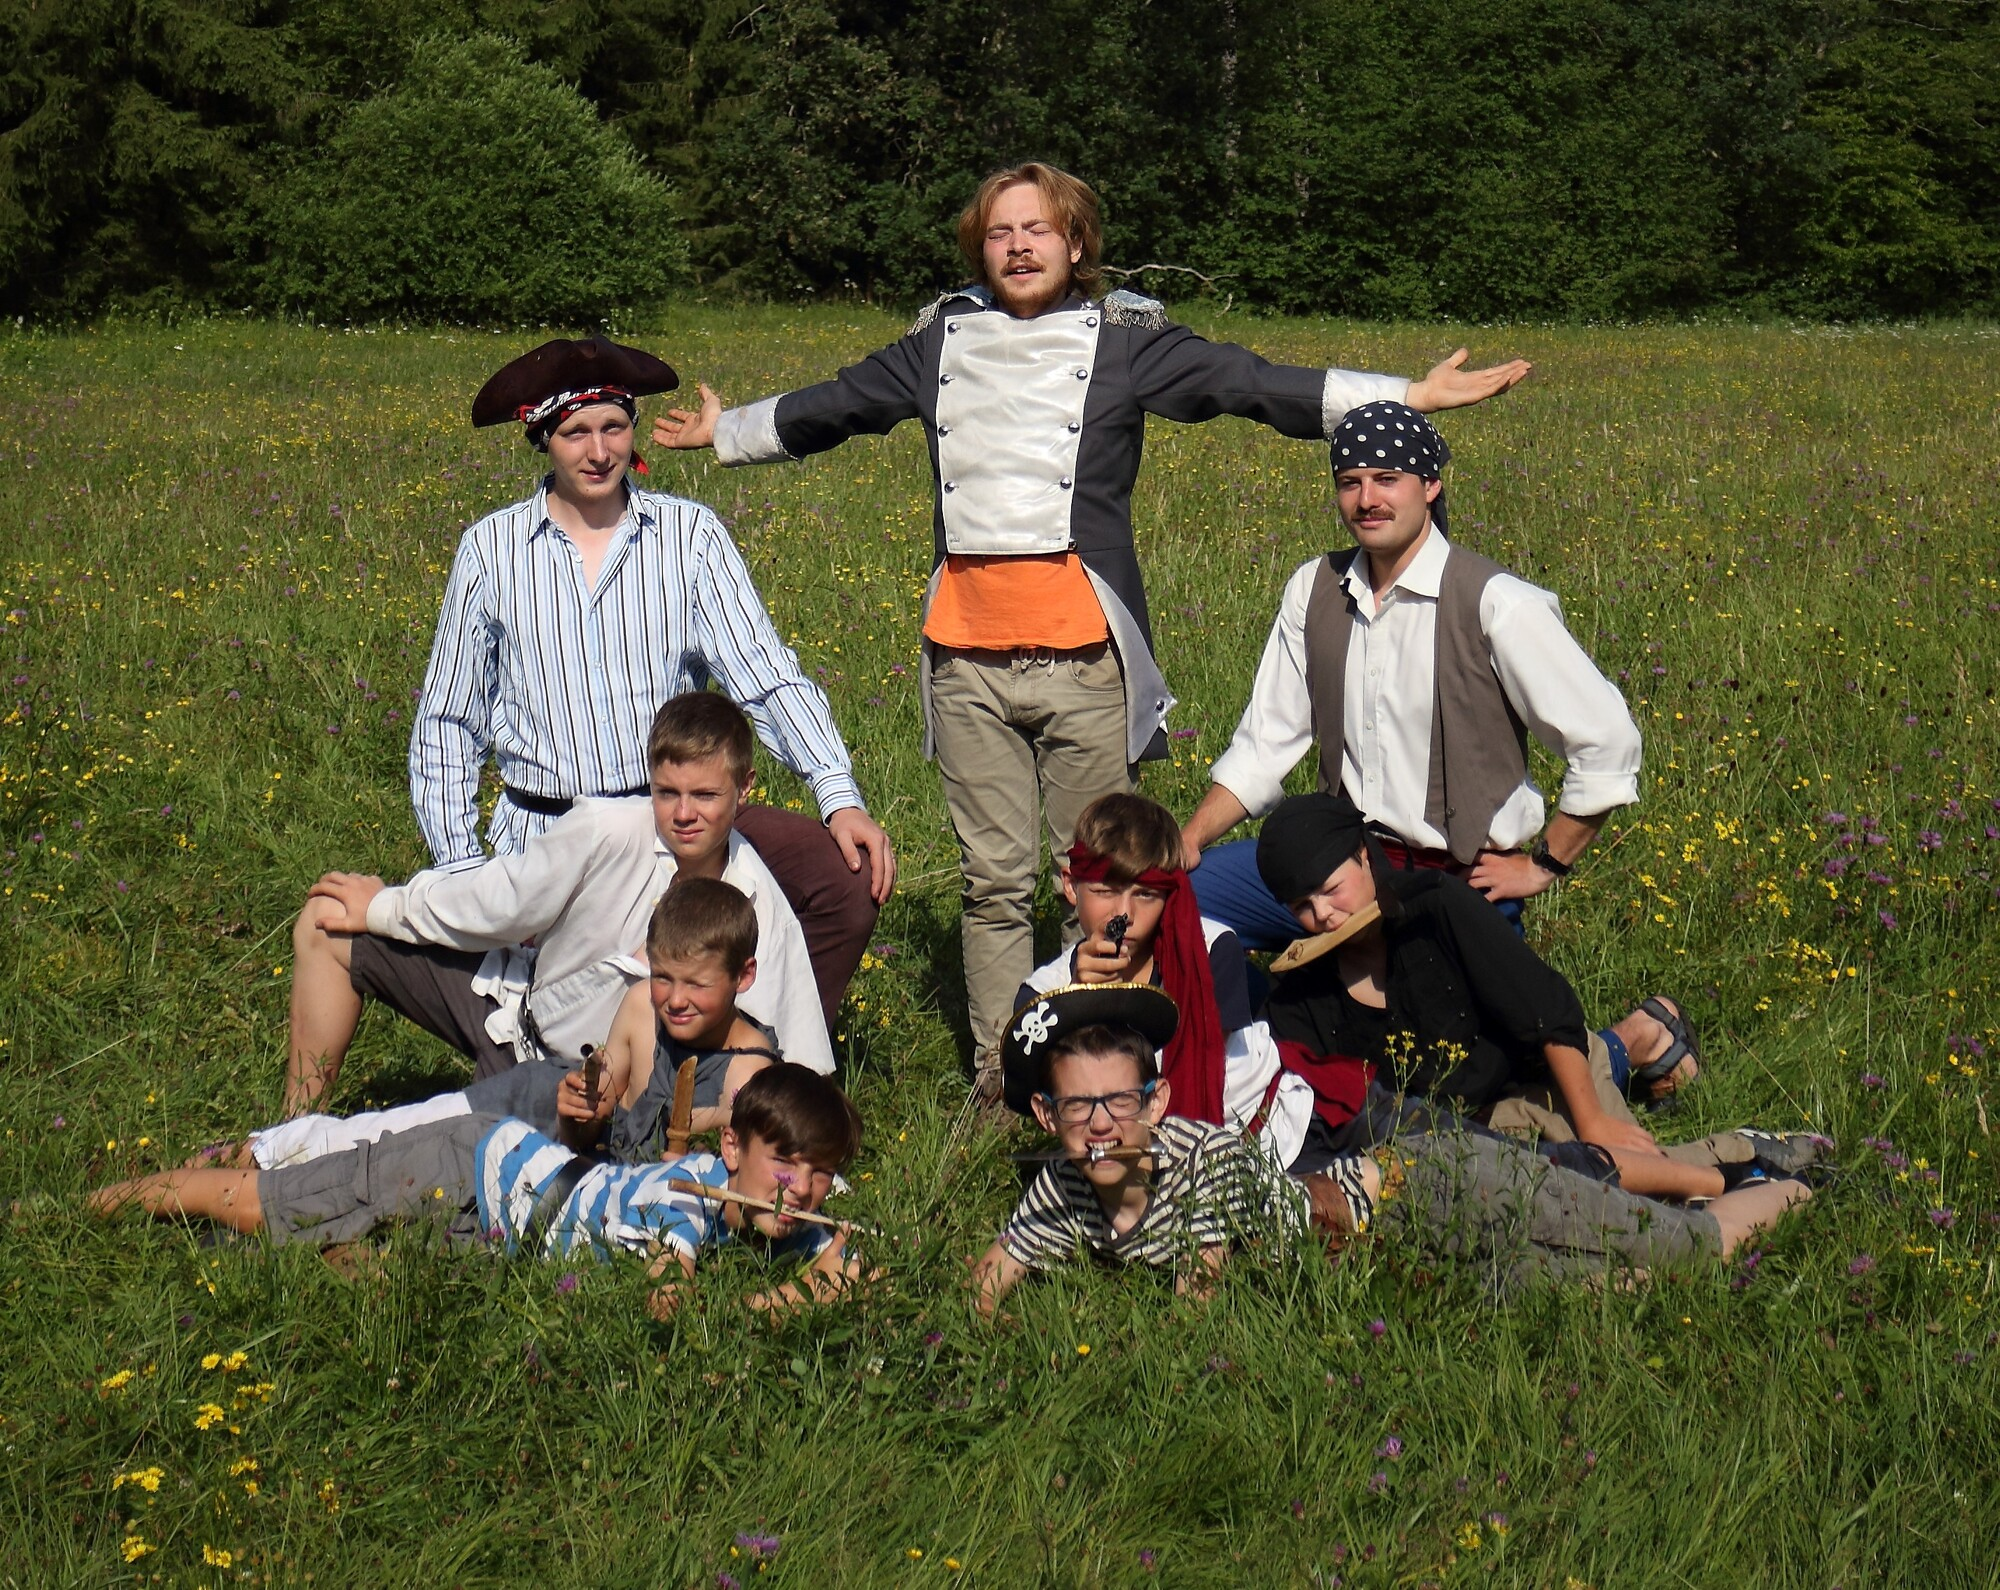
\includegraphics[width=10cm]{img/druziny/urzoni.JPG}

\end{center}

\clearpage

% subsection urzoni (end)

\subsection*{Borúwky} % (fold)
\label{sub:borúwky}

\begin{multicols}{1}

STAVEBKA:-)!\\
Jednoho dne jsme nastopili do onoho vlaku a odjeli na měsíc na jedno velmi neůtulné místečko k Ostrovci. Toto (pole) Louka byla velmi porostlá porostem. ze začátku se nám opoždila dovážka vody a mi jsme trpěli žízní. To byly asi 3 hodiny. Mezitím jsme dělali kolíky a matroš na kuchyň. Postavil se sněmák, nanosily bedny. Ustlali jsme si a dokonce jsme vyrazli i k “rybníku„ se umýt. Jstli vy co si to čtete si myslíte že jsme šli za sucha, světla, a tepla tak se šíleně pletete. Šli jsme za deště, zimy a za šera. Když jsme dorazili k okomu místu byla voda docela teplá. Když jsme se vraceli tak nám ostatní trocju utekli a já a Kája jsme za nimi v té tmě běželi po silnici. Druhého dne jsme pokračovali ve stavbě. Voda konečně dorazila a mi jsme se pustili do dalších prací. Mi jsme s Kájou a s Bendou kopali sklípek. Docela jsme si mákli a další den nás boleli záda. Stavba pokročila a mi už jsme měli postavenou kuchyň, latry a sklípek. Dále jsme vykopávali táboroví kruh O. Nejaký vedoucí (Alvis) nám ho zkrytizoval a na úkor toho jsme to museli velkou vrstvou zakopat. Všechno už bylo hotovo v ten onen den kdy ostatní přijeli. (Tedy maruška a Eskymáci s Urzony). To byla úleva (Jo a šlapali jsme bahno :) Hmm) ale to zas Jindy :)

\podpis{Jumbo:)}
	

MANÉVRY\\
Jednoho dne se na nástence objevil nápis MANÉVRY všichni si z toho dělali srandu ale odpoledne nás zavolala Cucumbrie a museli jsme odejít. Naše čtyř člená družinka (Jeden člen zůstal v táboře) šla do Ostrovce kde jsme potkali Debat a Šerifa. Spali jsme někde u Dědovic a ráno jsme museli jít asi pět kiláků.


Po cestě jsme neůzpěšně brodili takže jsme měli mokré boty ale dohonili jsme vedoucí a do cíle jsme došli asi o dvě hodiny dřív. Spali jsme kousek od nějakého hradu i s ostatníma družinkama protože jsme ráno měli dojít k hradu. 


Ráno jsme šli na hrad a na prohlídku a potom jsme šli k vodě kde přijeli piráti. Potom jsme dostali kousek mapi od Bezvousky a mohli jsme jít do tábora.

\podpis{Maruška}

VORVO\\
Byl nástup. Řekli nám že se máme převlíknout do oblečení které se může ušpinit. Potom nám svázali ruce ke klacku. Když jsme byli svázány odvlekli nás do vyschlého potoku. Všude byli spadlé stromy bahno a klacky. Museli jsme prolézt kus toho vyschlého potoku. Skoro všichni měli po kotníky bahno a ještě k tomu jsme měli pořád svázané ruce! 


Když jsme vylezli zavázali nám oči a odvlekli na další louku kde po nás házeli mouku. Potom jsme šli k pumpě u které nás nabarvili na modro. Když jsme byli nabarvený tak nám nabarvili zeleně vlasy. Potom jsme utekli k TP A vedle nich jsme hráli hru při které jsme se honili. Potom jsme šli spátky za ostatními. Byl to hustý pocit jak se na nás všichni koukali. A naše vlasy vypadali báječně!

\podpis{Kája}

\end{multicols}

\begin{center}

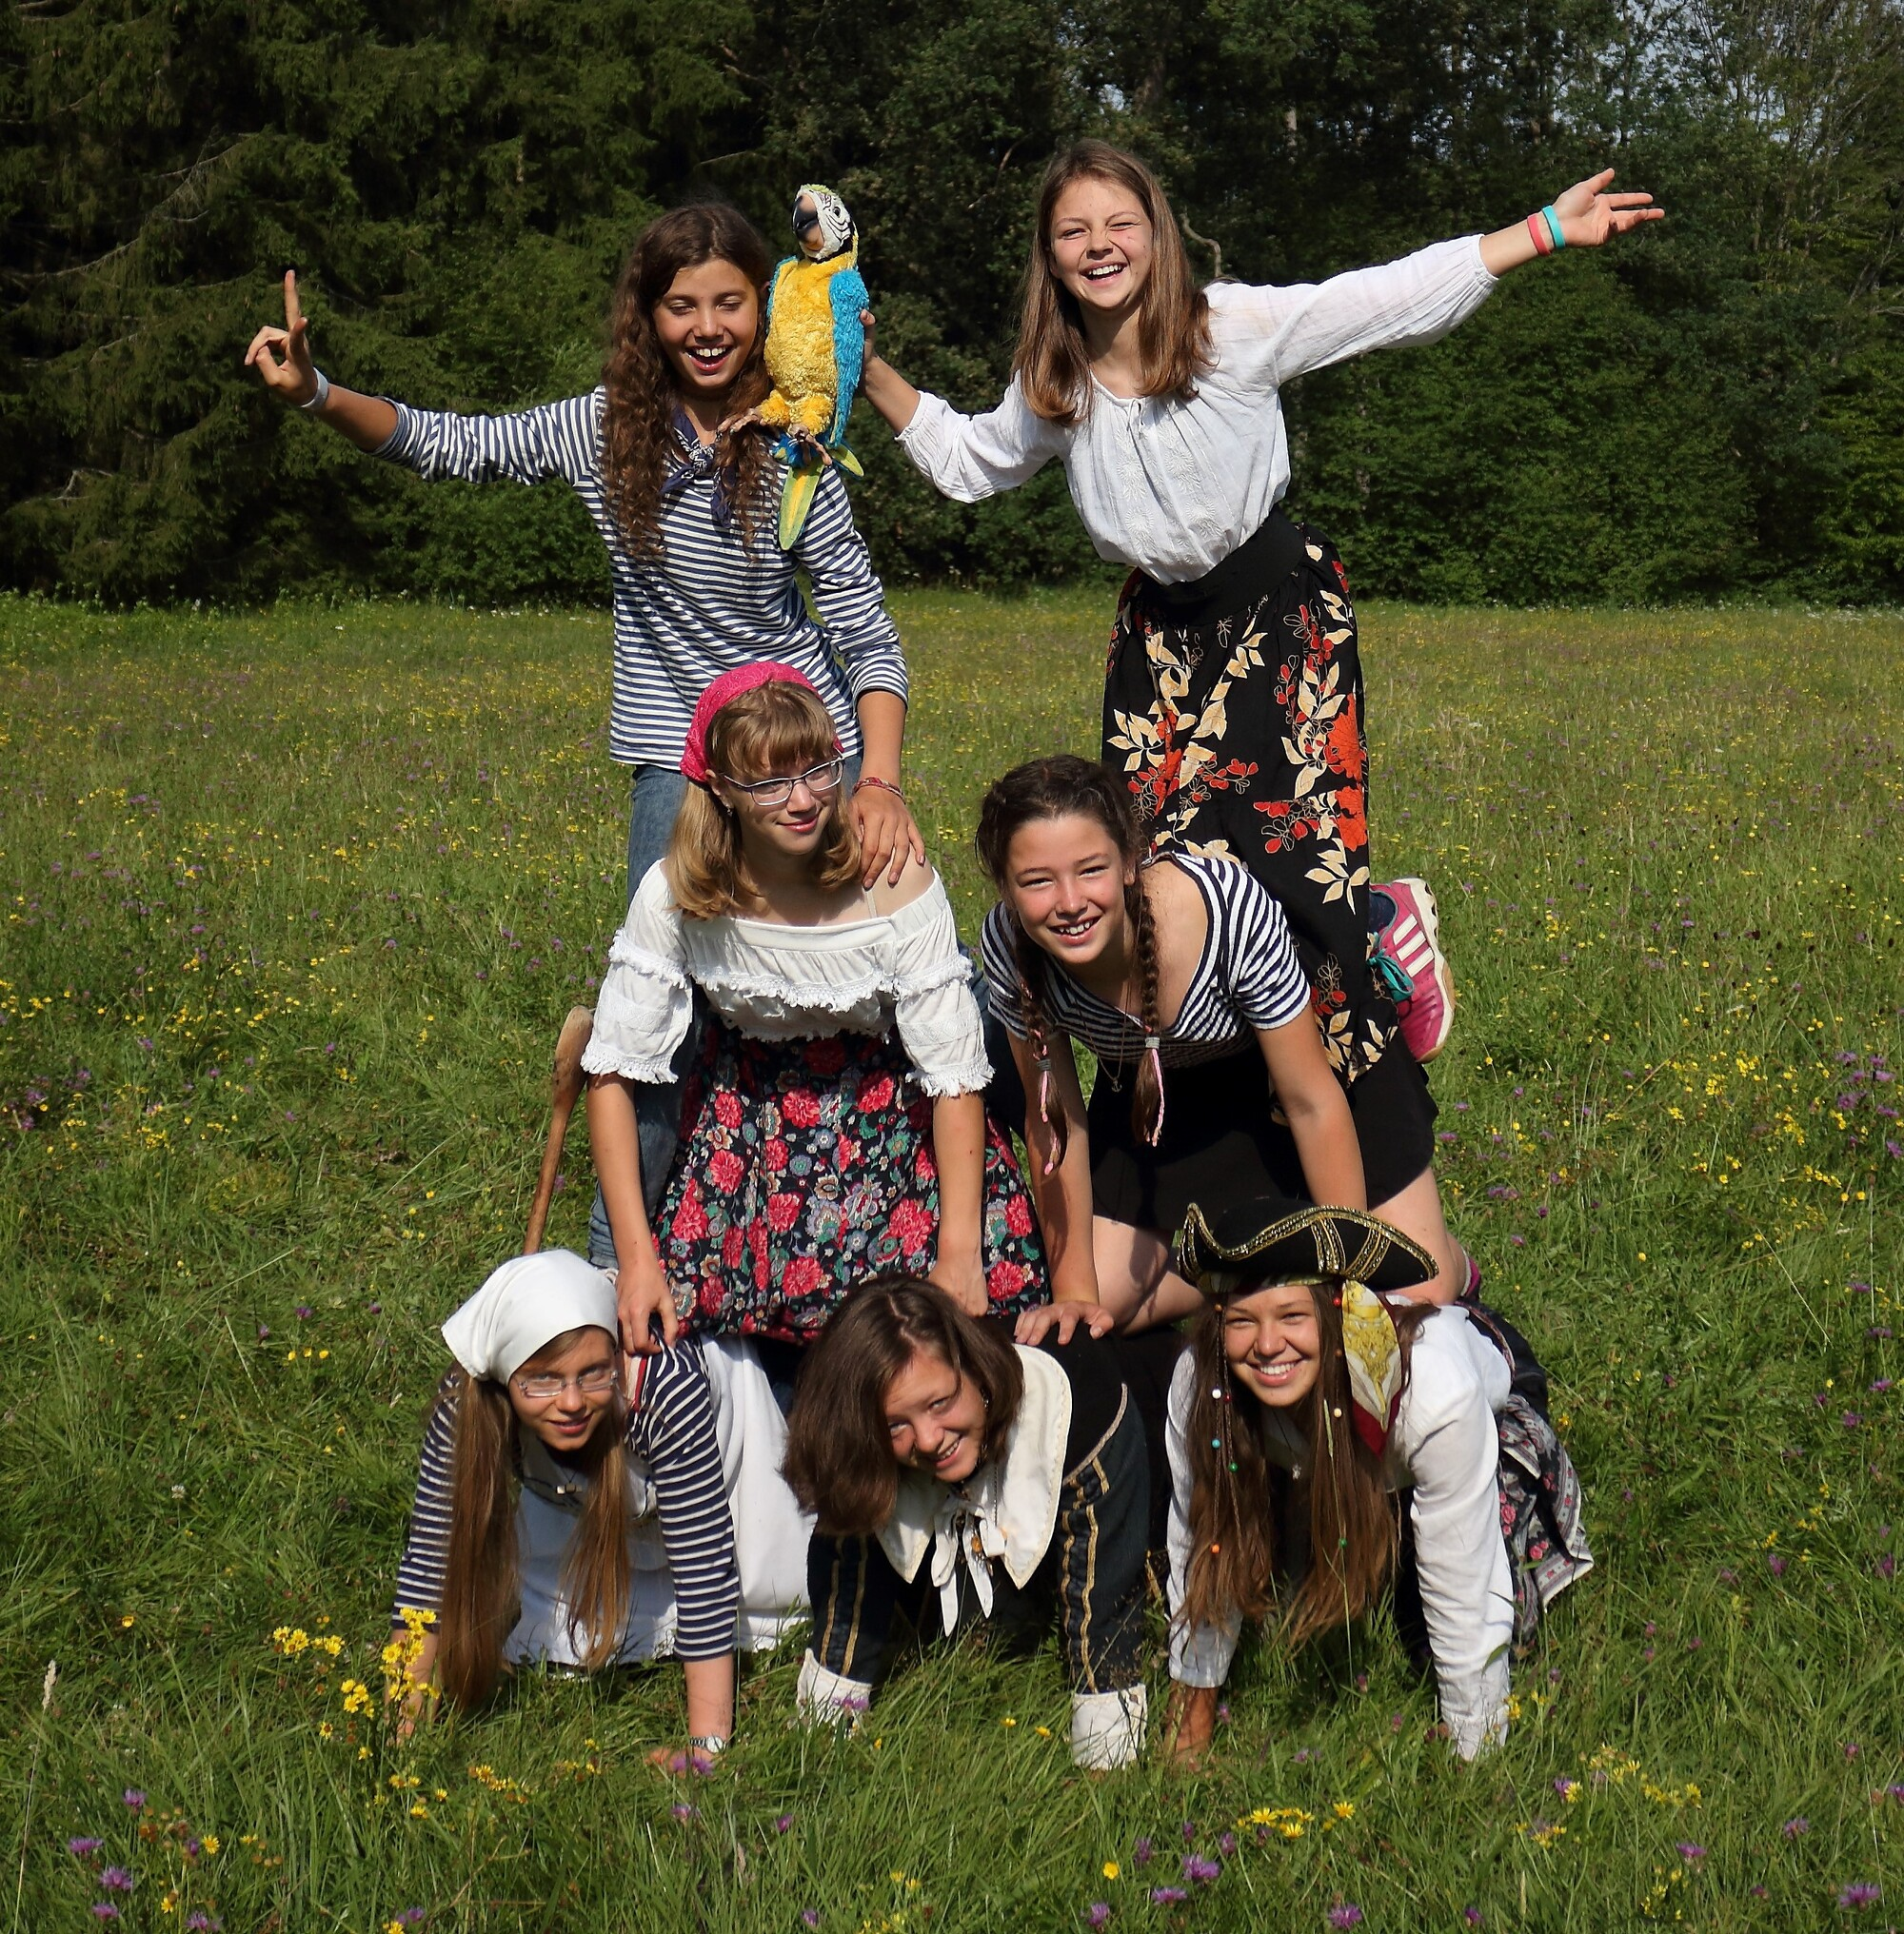
\includegraphics[width=9cm]{img/druziny/boruwky.jpg}

\end{center}

\clearpage


% subsection borúwky (end)

%boruwky sem

\subsection*{Pandakaty} % (fold)
\label{sub:pandakaty}

\begin{multicols}{2}
	

JSEM KAČKA, BAVÍ MNĚ HRÁT NA KLAVÍR
LÍBILO SE MI NA TROJDENCE ŠLAPAČKY DUPAČKY.

\podpis{Kačka}

JSEM HYPÍ A BAVÍ MNĚ PLÉST A ŠÍT.
LÍBILO SE MI JAK JSME NA TROJDENCE HRÁLY ŠLAPAČKY DUPAČKY.

\podpis{Hypí}

Já jsem Jája, líbí se mi jak jsem zachraňovaly Wendy. Nelíbilo se mi když budu mít přepad. (hlídku-poznámka redakce)

\podpis{Jája}

\columnbreak

JÁ JSEM TUKI. MNĚ SE LÍBÍ GDIŠ SME KAMARÁDI, ALE NELÍBÍ SE MI GDIŠ BUDU HLÍDKA.

\podpis{Tuki}

JÁ JSEM BÁRA
MŮJ NEJLEPŠÍ ZÁŽITEK BYL JAK JSME NA TROJDENCE OPÉKALY BUŘTY.

\podpis{Bára}


Já jsem Tóna a nejvíc se mi líbilo jak jsme hrály opičí dráhu. Byly sme s Lucinkou na druhým místě.

\podpis{Tóňa}



VANY TRÁVNIKOVÁ
MÁM RÁDA PALAČINKY 
MÁM RÁDA HRY A VÁNOCE 
LÍBÍ SE MI ŠLAPAČKI DUPAČKI

\podpis{Vany}
\end{multicols}

\vspace*{15pt}

\begin{center}

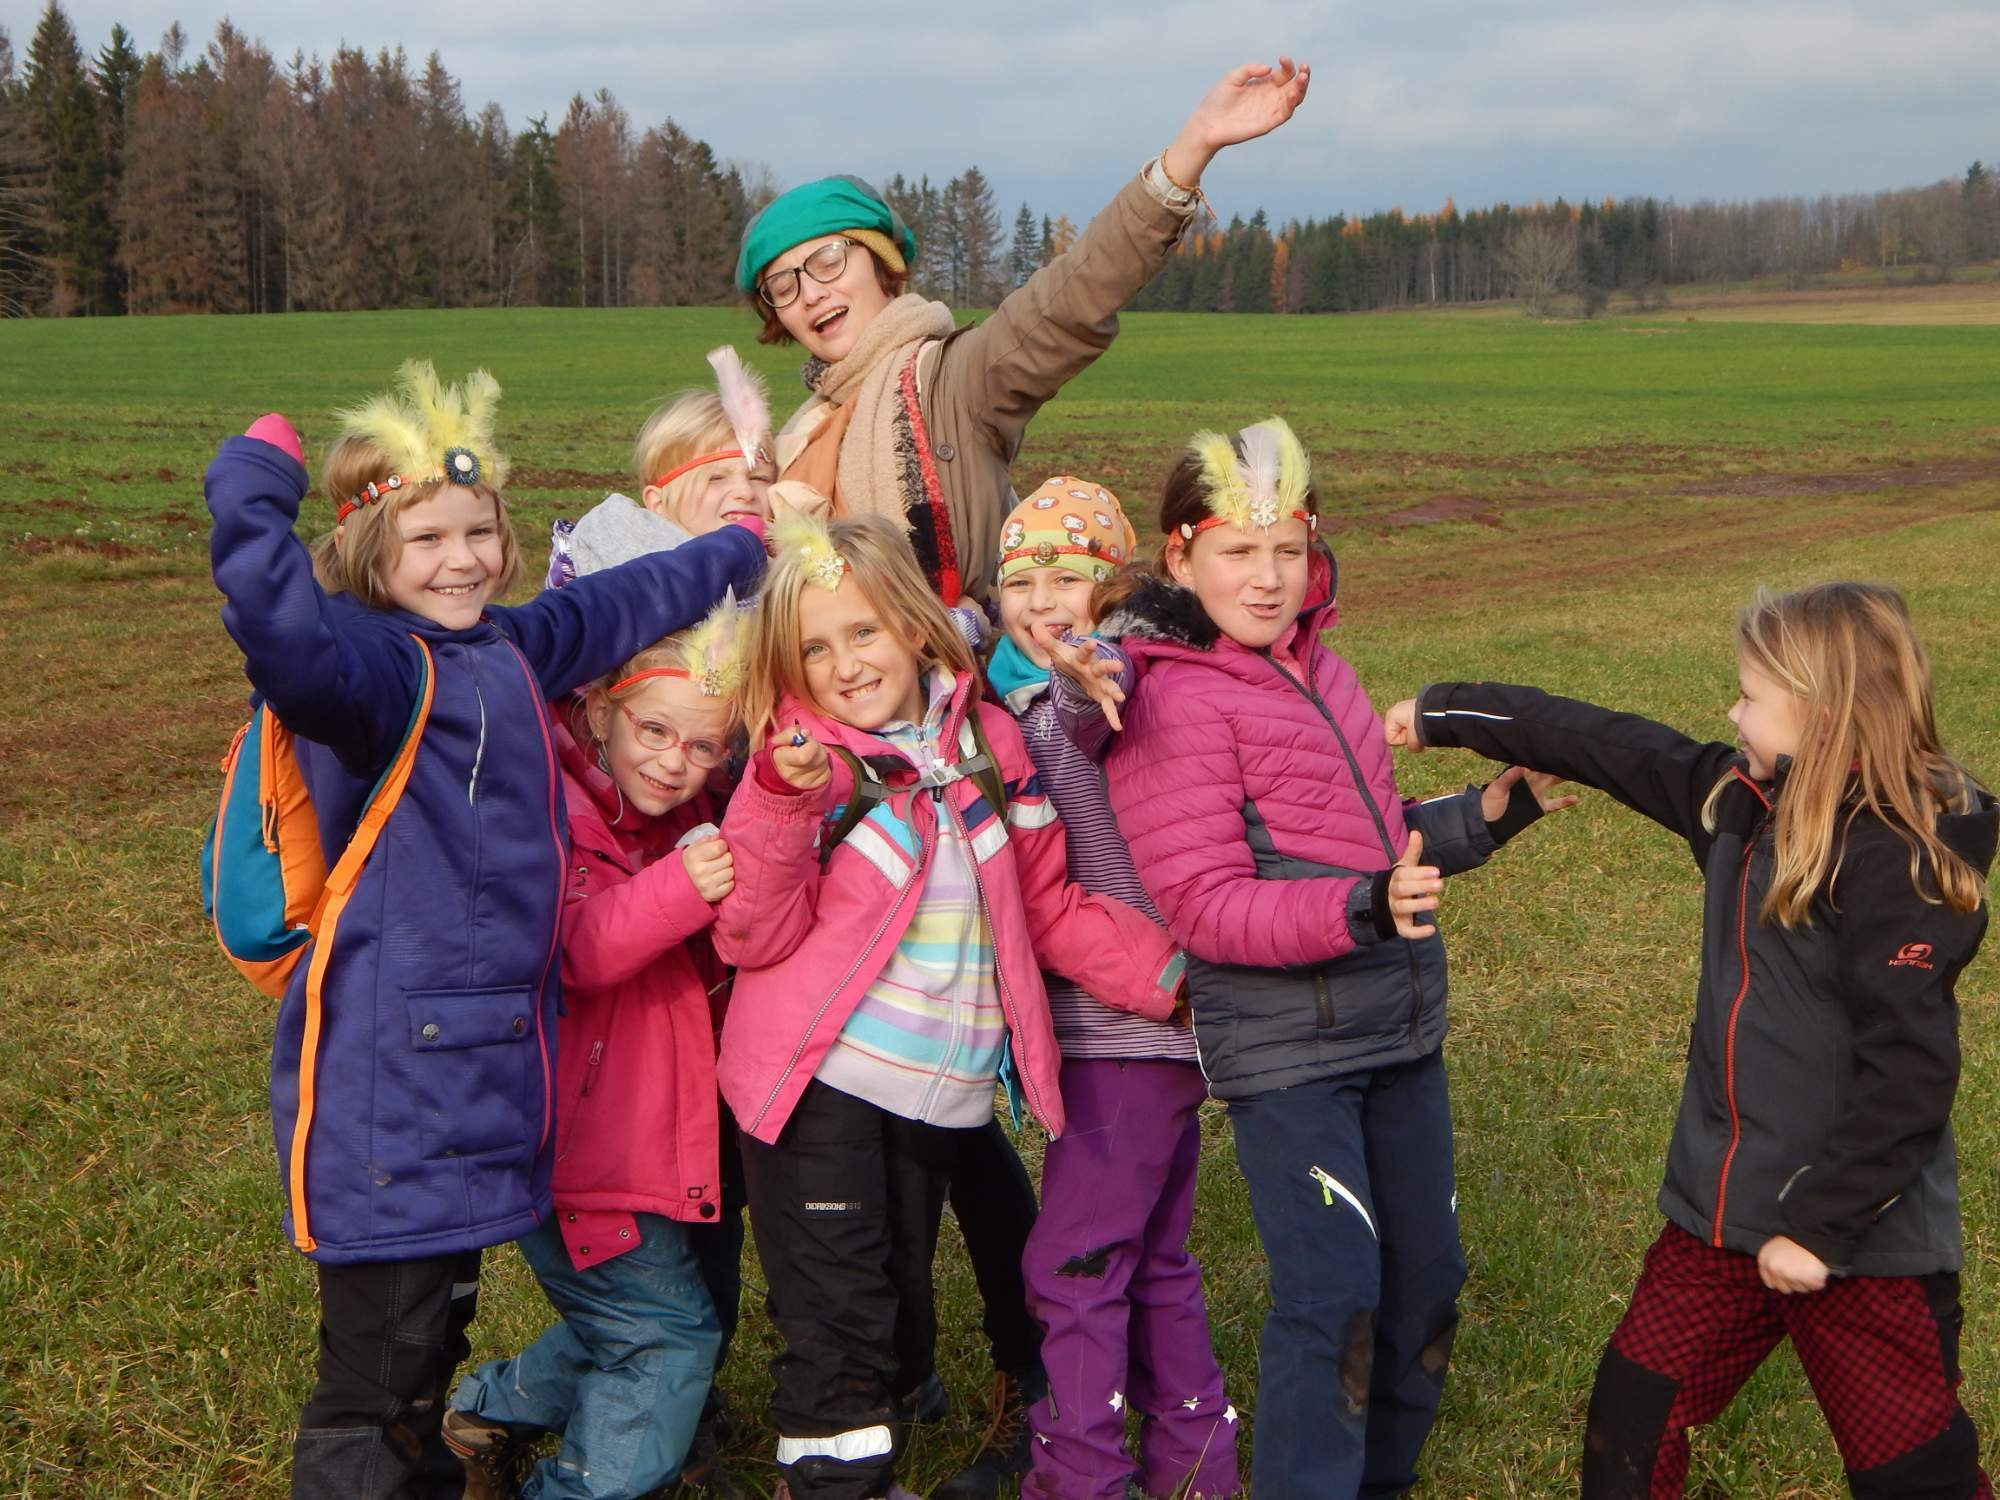
\includegraphics[width=10cm]{img/druziny/pandakaty.jpg}

\end{center}

\clearpage


% subsection pandakaty (end)
\subsection*{Kočičáci} % (fold)
\label{sub:kočičáci}

\begin{multicols}{2}

ZASPAL JSEM NA PŘEPADENÍ. BILA SUPER KOLÍČKOVÁ. ŠLI JSME V BAHNĚ A NAŠLI JSME ČOKOLADU. BILA SUPER HOSPODA.

\podpis{KRATER}




BYLO TO TAK ŮŽASNÝ KDYŽ JSME SE SNAŽILI PŘEPRAT INSTRUKTORY A SE MNOU UDĚLALI DOUBLEKILL. RÁD JSEM CHODIL NA PROCHÁZKY A POTKAL JSEM ROZTOMILÍ KOTĚ A CHODILO ZA NÁMA STRAŠNĚ DLOUHO. VIDĚL JSEM HODINY KTERÝ VIPADALI JAKO PIZZA A MISLEL JSEM SI ŽE JE TO PIZZÉRIE.NA PROCHÁZCE BYLI ZAVŘENÝ ZÁVORY HODINU A VLAK NIKDE TAKŽE JSME TO OBEŠLI A ZA MINUTU JEL VLAK. BYLI JSME V MALÍ AMERICE A JEDLI JSME MARŠMELOUNY.

\podpis{DOMČA}



BYLI JSME 1. LÍBILI JSE MI MANEVRI. LIBILO JSE MI TABORAK ŽE SE POSILALI SLATKOSTI. ZASPAL JSEM A OŇI ZAŤIM CVIČILI ROSVIČKU. A LÍBILO JSE MI Ž PO OBĚDE JSME HRÁLI FOTBAL. LÍBILO JSE MI HOSPODA A POLÍVALI JSME SE ČAJEM. A BYLI JSME V BAHNE. BYL PŘEPAD1. MNEŘILI JSME SI SVALI PILOU. HRALI JSME DRAČÁKA.

\podpis{VRINGU}

\columnbreak

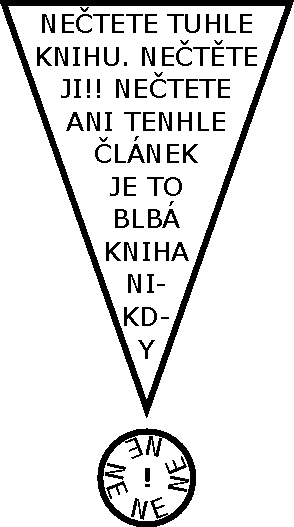
\includegraphics{prispevky_deti/paradox.pdf}

\podpis{PARADOX}



LIBILI SE MI MANEVRI BIL JSME 1. BILI SKVELI SKOUŠELI JSME DRSNAK BONUS ALE SPLNILI SME HO JENOM DVA DNY BYL TEŠKI HODNĚ SE MY LIBILI. HRALI JSME SKVEL HRY OHĚN BIL SKVELI AŽ NA TO ŽE MUSELI SBIRAT MALI VETVE ALE A BYLI STEJNE MĚ TO BAVILO A BYL ŠMOLUIPROGRAM BILI JSME 1. A TAKI ŽE BILY HOSPODA HODNE SE MI LYBILO HRA O PREŠITI LIBILO SE MI DELAT PŘIŠLO MI TO HUSTI MYNIMANEVR MELI SME JIT DO HRADU POTOM JSME MILI JIT DO LASA A PŘESPAT V TOM LESE BILI BILO HODNĚ ODNE ZIMA KOUPANI V ŘECE BILA LEDOVA ALE NIKDY JSEM SE NEPŘIVLK AVDICKY JSEM SEM PLAVKI POD KALHOTAMA ATAKI ME TO VŠECHNO BAVILO BEZVIJIMKY MEL JSEM DOBROU NALADI HODNE SE MY STISKALO HODNE SE MY LIBILO MAMCE A TATOVI. BILO TO LEPŠI NEŽ JSEM SI MISLEL DOBRI BILO TAKI HODNE BAVILO KDIŽ SME SE BAVILO KDIŽ JSME SE PŘITAHOVALO NA STROM.

\podpis{HROMDOPOLICE!}


	
\end{multicols}
\begin{center}

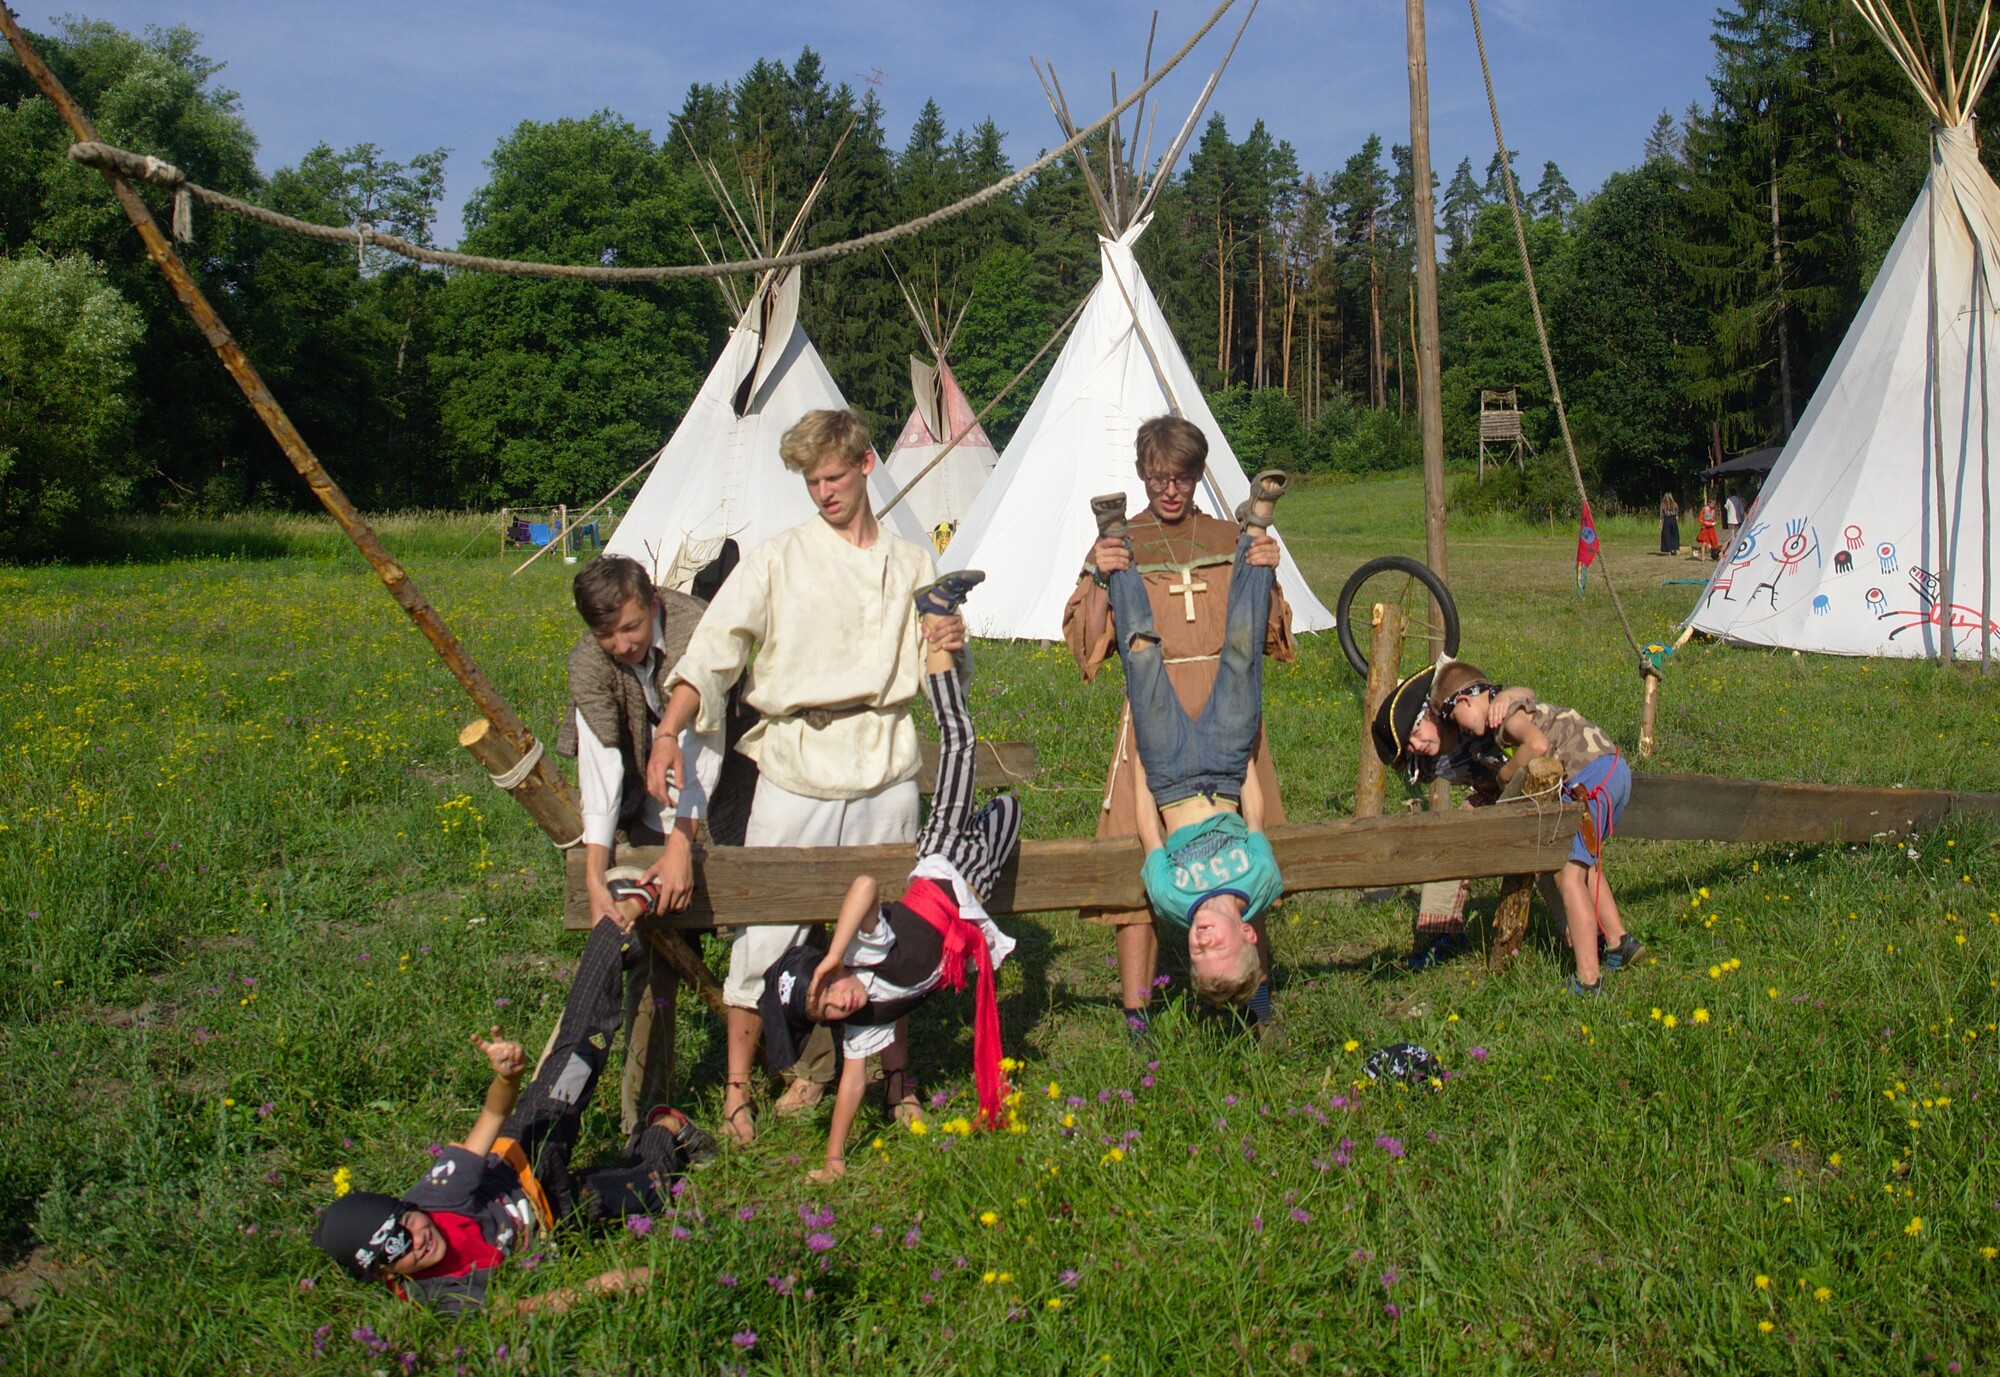
\includegraphics[width=10cm]{img/druziny/kocicaci.jpg}

\end{center}

% subsection kočičáci (end)
\subsection*{Jejdové} % (fold)
\label{sub:jejdové}

\begin{multicols}{2}
	


Mini manévry\\
První den tábora po obědě nám stavebkářům řekli, že si máme zabalit na přespání. Poté jsme se vydali do Ostrovce na nádraží, kde jsme se setkali s ostatními, kteří přijeli vlakem. Poté přišli mnich a sedlák a ti nás rozdělili do dvou skupin a rozdali nám kusy prádelky, na kterou jsme si pověsili vše potřebné vše potřebné na přespání, takže např. spacák, karimatku, pití a kartáček na zuby. Prádelku jsme si pověsili buď kolem pasu, nebo na rameno. Poté mnich a sedlák každé skupině dali popis cesty a my se vydali vstříc cestě. Cesta ubíhala dobře, až jsme se dostali do bodu zlomu. Rozdělili jsme se na dvě skupiny. Jedna chtěla jít rovně a druhá doleva. Nakonec vyhrála skupina vlevo. Tak jsme se po půl hodině improvizování dostali do vesnice… Ostrovec. Tam jsme zavolali na číslo na našem papíře a dovolali jsme se překvapivě do tábora. Když jsme jim oznámili, že jsme se dostali opět do Ostrovce, byli velice překvapeni. Poradili nám a doplnili jsme zásoby vody a opět se vydali na cestu. Když jsme se opět dostali do onoho bodu, tentokrát jsme se vydali rovně a po chvíli jsme se chytili popisu. Podle něj jsme pokračovali asi do tři čtvrtě cesty, kde jsme najednou potkali druhou skupinu, která se u silnice a nevěděla kam dál. Poté jsme podle popisu pokračovali až do obce Zvíkov. V obci jsme se měli vydat podél tří hostinců a dvou tee-pee. Po chvíli jsme narazili na paní a po dlouhém rozhovoru s ní jsme zjistili, kde bydlí pán, který staví tee-pee. Ten nám řekl, že právě dvě tee-pee stojí u dětského domova a ukázal nám cestu. Po chvíli jsme se dostali k rozcestí dvou cest a opět jsme nevěděli kam dál. Opět jsme se rozdělili na dvě skupiny a jedna zůstala na rozcestí a druhá, ve které jsem byla i já, se vydala hledat dětský domov. Po pár minutách jsme došli k policejní stanici, před kterou stáli dva policisté, a já se bez rozmýšlení jednoho z nich zeptala, kde je tu dětský domov a oni nám řekli kudy. A tak jsme se konečně dostali k dětskému domovu a já se vydala pro druhou skupinu, ale jinou cestou, která měla být rychlejší. Po chvíli jsem se dostala k rozcestí, kde měla druhá skupina čekat, ale nebyla tam a tak jsem se vrátila k dětskému domovu a naštěstí druhá skupina za chvilku dorazila. Společně jsme se vydali dál k hradu Zvíkov. Tam nás po chvilce hledání našli mnich se sedlákem a společně jsme si dali večeři neboli chleby s májkou. Při večeři nám vyprávěli, že lidé co zde žijí, jsou zapřisáhlí monarchisté a jelikož jsme demokrati, tak jsme museli odtamtud co nejrychleji odejít a tak jsme hned po večeři vyrazili do lesa kousek od hradu a tam se utábořili. Ráno nás vzbudil voják, který přišel sebrat mnicha jako vzbouřence proti režimu. Když z nás opadl šok, přišli muž a žena, kteří se představili jako Namežan a Žužuman Delaff. Ti nás pozvali na svoji loď, na které budeme podnikat cesty do různých koutů naší země a přesvědčovat lidi, aby podporovali demokracii. A tak jsme se se sedlákem vydali na, teď už i naši, loď neboli do tábora. A toto byl stručný zápis událostí prvních dvou dnů našeho tábora.

\podpis{Mrkev}



Letos jsem si hodně užila tábor. První den jsme vyrazili na "minimanévry" . Byli jsme na hradě Zvíkově aby jsme zachránili demokracii před monarchií. Jako piráti jsme se snažili aby monarchisté pochopili proč chceme demokracii. To se nám na konci tábora podařilo, pomocí elixíru pochopení.
První trojdenka byla s kibitzem. Na trojdence jsme velice zapojili svou fantazii.
Byli jsme tam i s Borúwkama. Kája a Zubejda přijeli pozdě, ale přivezli dort,(protože Kája měla narozeniny).Trojdenku i dort jsme si všichni užili.
Na další trojdence jsme začali celoroční téma u kterého nás měla provádět kniha: Kronika rodu Spiderwicků. Za celou trojdenku jsme přečetli dva díly. Hlavní pointou trojdenky bylo zahnání zlého polykače na dvacet let do podsvětí. Zahánění polykače jsme absolvovali my osobně a aby polykač neřádil ve městě moc dlouho i za dalších třicet let , kdy už bude moct znovu opustit podsvětí tak jsme jedné místní paní dali instrukce aby i ona (nebo její potomci) mohla vykonat rituál. Až když jsme předali poselství tak jsme se s klidem mohli vrátit do svých domovů.

\podpis{KECKA}




Půlnoční esej\\
Tento tábor jsem slibovala na skauta.
Na přípravách jsme se dozvěděli že musíme napsat esej na to proč sechceme stát skautem.
A čas plinul za pár dnů byl čas odevzdat esej.
Já Zubejda a Penny jsme to měli napsané ale mě a Penny se esej stratila. Už byl večer a byli přípravy a popravy.
Tuto přípravu jsme měli už odevzdávat esej až na to že já a Penny jsme jí pořád neměli. Potom na přípravě nám vedoucí řekly že to tolik nevadí a že to ráno musíme odevzdat.
Po večeři zjistila že mám hlídku a po mě hned Lochneska a rozhodla jsme se že poprosím Lochnesku jestli bych s ní nemohla zůstat na hlídku abych mohla napsat esej.
Když jsem přišla do týpka tak mě poprosila Penny jestli bych ji nevzbudila až budu budit Lochnesku tak jsem souhlasila. Ke konci mé hlídky jsem šla vzbudit Penny i Lochnenesku. Teprve ke konci Lochnesčiný hlídky jsen dopsala konečně esej. Lochneska prosila jestli bych tam sní ještě nezůstala ale už jsem byla moc unavená. tak jsem šla spát.


\podpis{asi Zpátečka}


Zážitku z táborů je velmi hodně bylo těžké se rozhodnout o kterém napíšu . Ale vybrala jsem si noční hru z tábora ( téma: piráti ). Měli jsme jenom přejít křižovatku a zahnout doprava. Nebylo to ale tak lehký protože jsme šli po jednom a museli jsme se plazit. Nebo alspoň být jenom zkrčený. U ty křižovatky však byli něací opilí piráti ( nebo nevim kdo to byl). Takže jste museli být potichu aby vás neslyšeli a nechytli vás. Když jste odbočili tak jste pak šli chvíli po pěšince než jste na někoho nenarazili.

\podpis{Zubejda}

\columnbreak

Příspěvek do knihy Keya
Tento rok jsem si vážně užila! Ráda bych řekla něco o táboře. Když jsme přijeli do vesnice Dolní Ostrovec, nešli jsme rovnou do tábora, ale byly tzv. minimanévry. Naše skupinka to nějak popletla a skončili jsme zpátky v Dolním Ostrovci:) Nakonec jsme přespali poblíž hradu Zvíkov a ráno jsme šli do tábora. Ten den bylo snad naposledy slunce (teda kromě konce tábora). Stavění a dodělávání tee-pee se protáhlo na déle než bychom čekali. Na tomto táboře se nikdo neobešel bez štípanců od vos a komárů. Ale i přes otravný hmyz jsme na táboře s tématem Piráti opravdu užili spoustu zábavy a mě překvapilo že Vařící etapka byla téměř na začátku tábora. Poté byl čas na Skautské přípravy a popravy. Chtěla jsem na konci tábora skládat Skautský slib a psala jsem esej na téma proč chci být Skautem. Jenomže den před termínem odevzdání jsem ji ztratila a musela jsem ho psát na hlídce! Ne na mojí, ale na Lochnessčinu. Potom byly manévry. Byly vážně super včetně toho, že jsme nemuseli nikam hnát. Po návštěváku se na oblohu opět dostalo slunce a bylo teplo. Ale vyskytl se další problém. Jaksi nám nevsakovala vsakovačka, tak jsme ji s Jejdama vylévaly a našli jsme mrtvou myš! Udělaly jsme jí patřičný pohřeb a ozdobili jí hrob. Následující pokladovka se mi moc líbila. Potom přišel čas na 3. táborák a slibování, stala jsem se Skautkou a všichni jsme spali u táboráku. Moc jsem si to užila a děkuji všem vedoucím za skvělý tábor.

\podpis{Penny}


\end{multicols}

\begin{center}

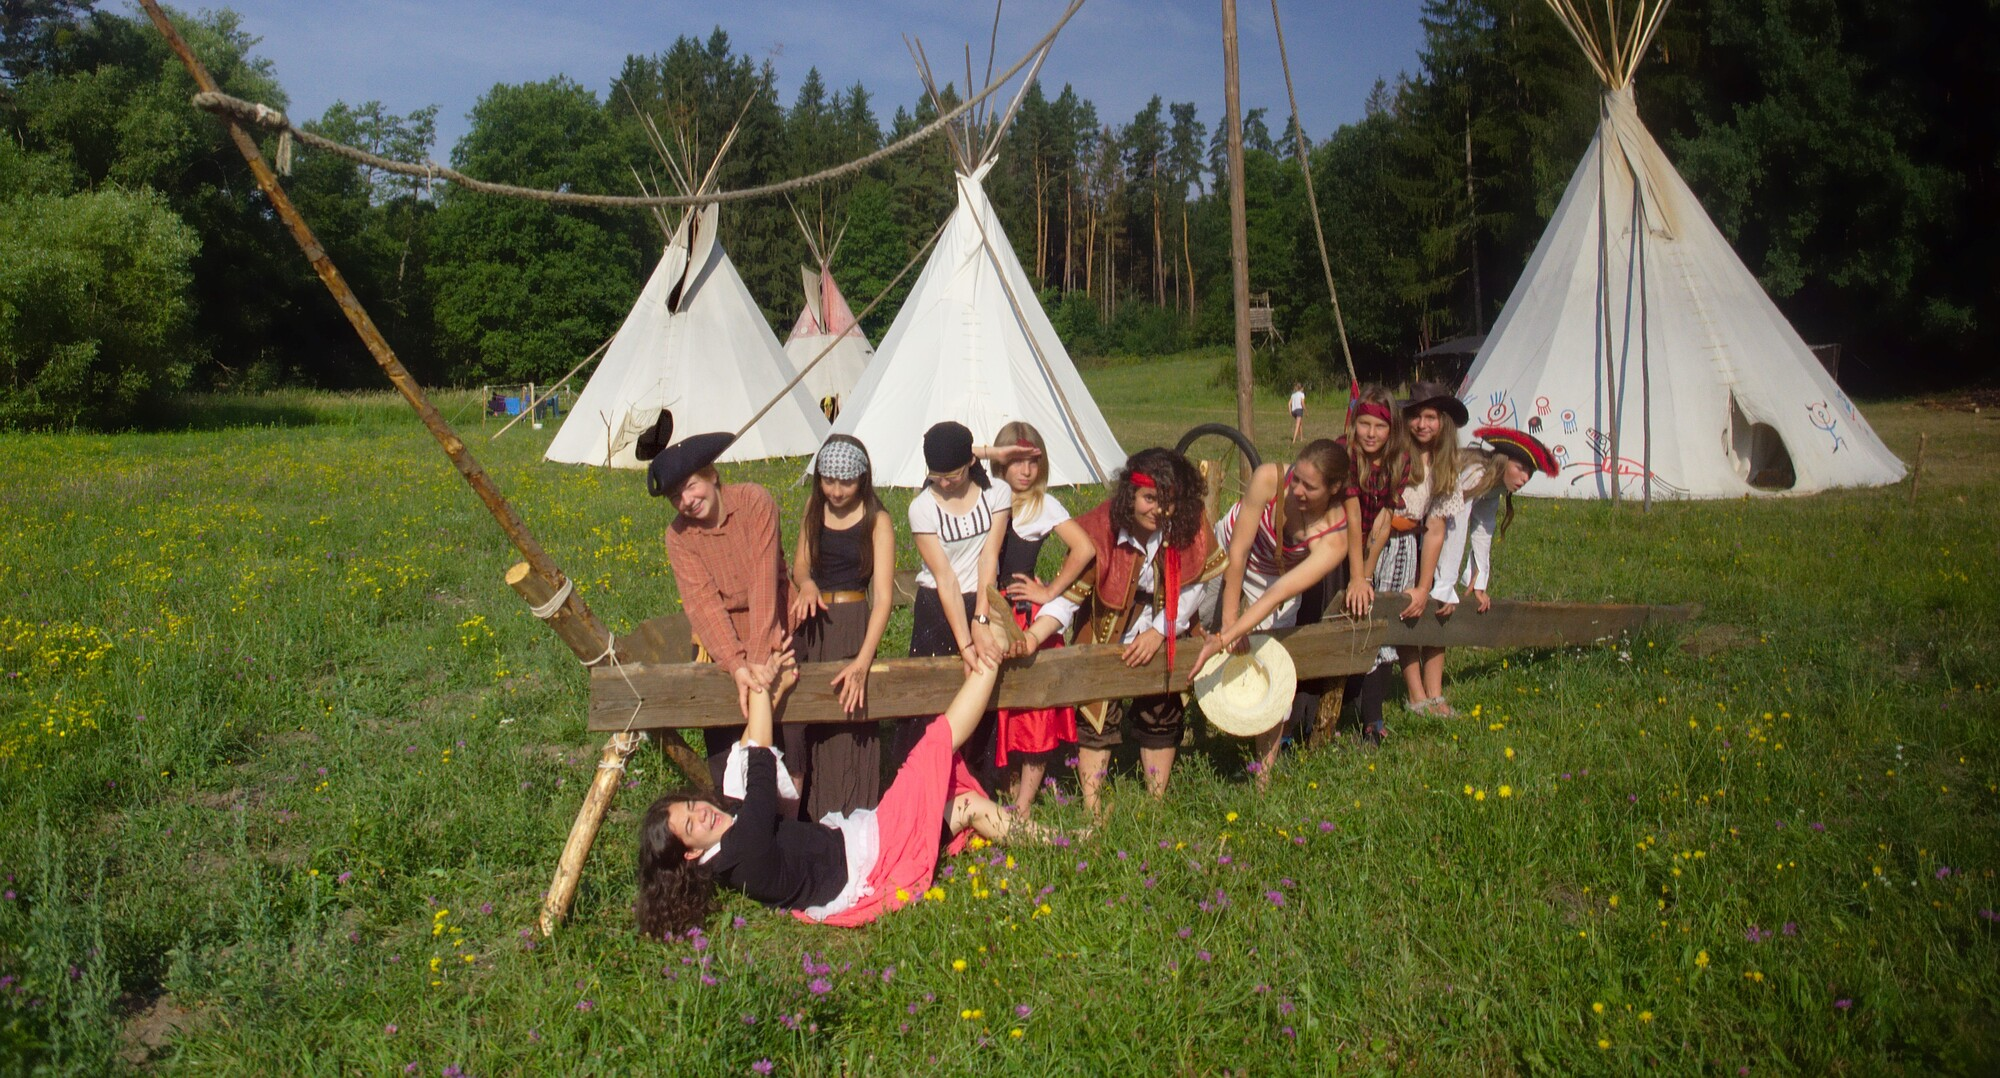
\includegraphics[width=10cm]{img/druziny/jejdove.jpg}

\end{center}


% subsection jejdové (end)
\subsection*{Axolotli} % (fold)
\label{sub:axolotli}

\begin{multicols}{2}

Na samotce byla nuda. Bylo tam tolik komárů a vos jako Somálců v budce když tam hodíš piškot. Na DVD jsme udělali fakt hodně pudinku a nikdo ho nechtěl  stejně jako na manévrech, kde jsme udělali fakt hodně pudinku ve kterym byly úplně nechutný sušený, ale znovu rehydrovaný banány. Vyhráli jsme bodování a jako odměnu jsme dostali utopence...
P.S. Linux je lepší než Windows

\podpis{Einstein}




Tři orlí pera- samotka:\\
Rád vzpomínám na tábor. Na tomto táboře jsmem se jeden den nejvíc nudil a to bylo poslední zkouška třích orlích per, byla to zkouška samotky. Byla to hrozná nuda, spal jsem asi do desíti hodin přes noc mi kus chleba sežrala myš kterou jsem pak večer viděl. Tři orlí pera jsem udělal.

\podpis{Bobeš}

\columnbreak

Rád vzpomínám na tábor. Na tomto táboře bylo nejzajímavější, když jsme měli družinkáč. Bylo to zajímavé, protože Einstein a H-hruška drželi hladovku a já jsem mlčel. Tak jsme čekali až do půlnoci a pak jsme začali smažit řízky. Jídlo jsme jedli na mé a Einsteinově hlídce. Bylo to moc dobré. Jsem moc rád, že nám uďové dovolili na družinkáči řízky.

\podpis{Picasso}


Rád vzpomínám na tábor. Jedna z věcí na kterou rád vzpomínám je genderový program. Program měl na starosti Hafík a Kibitz. Ty nám připravili workout a jiné mužské záležitosti. Ze začátku jsme “posilovali”. Poté jsme šli sbírat proteiny. Jako proteiny jsme vzali kobylky. Následně jsme je usmažili. Podávali se buď na sladko nebo na slano. Na konec se pořádali řeckořímské zápasy.

\podpis{Hahruška}
\end{multicols}

\begin{center}

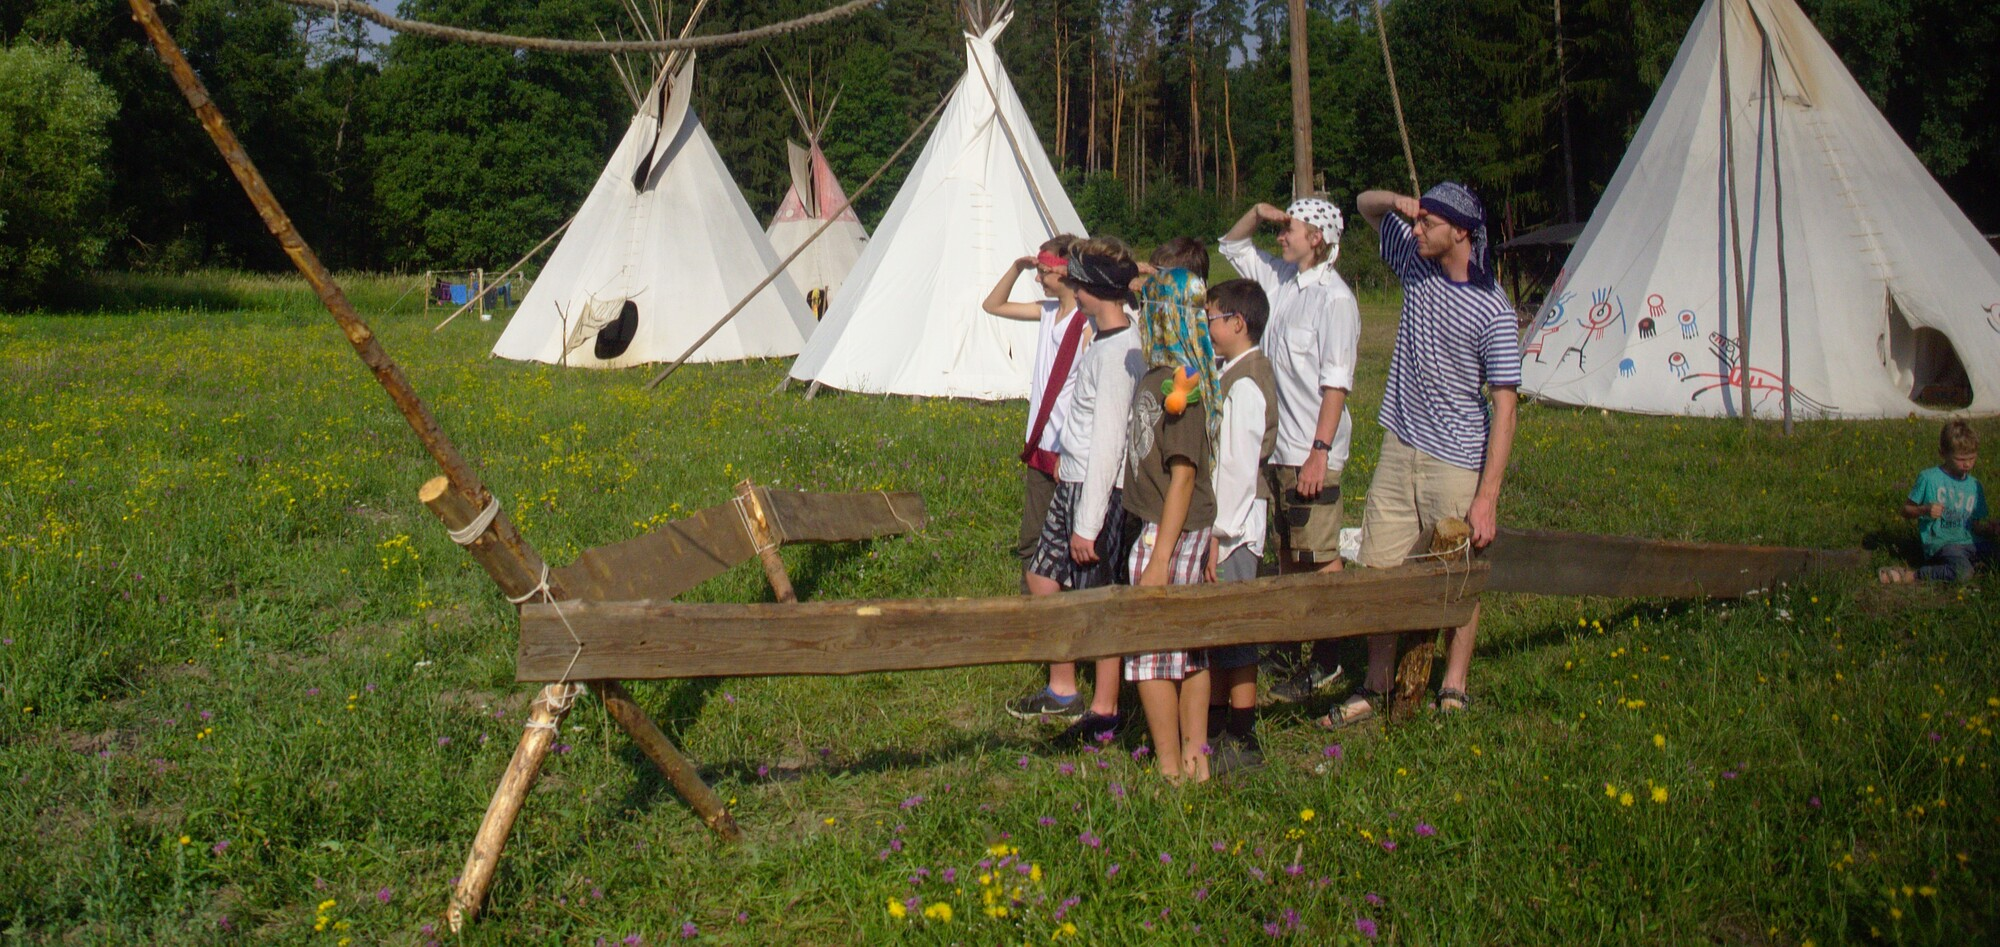
\includegraphics[width=10cm]{img/druziny/axolotli.jpg}

\end{center}

%\clearpage

% subsection axolotli (end)

\subsection*{Ještěrky} % (fold)
\label{sub:ještěrky}

\begin{multicols}{2}


Tábor jsme si jako Ještěrky moc užily. Snad poprvé v historii jsme se tam sešly všechny. Vychutnávaly jsme si chvilky v přírodě. Konečně se nám zase podařilo uniknout pryč od toho pražskýho stereotypu a městskýho života. Moc ráda budu vzpomínat např. na klidné manévry s mojí etapkovou skupinou. Z Ještěrek jsem byla s Olivou a E.T. a moc jsme si užily společný čas. Jediné, co by celkovému dojmu z tábora snad ještě přidalo, by byl blýzký potok. Mohu potvrdit z vlastní zkušenosti, že tekoucí voda z pumpy se nedá s proudem chladivého potaka či říčky vůbec srovnávat. Avšak i přes tento malicherný nedostatek jsou mé pocity ohledně prázdnin strávených na táboře kladné.
\podpis{Viki}


Pro mě byly velmi příjemné relaxační akce, už jen z toho důvodu, že tyto programy obsahovaly všechno, jen ne práci a nepohodu.
Ale co to vlastně takova relaxační akce je? 
Když bylo moc velké horko, a když říkám velké, myslím tím ultra mega velké, tak nám vedoucí řekli, ať si vezmeme plavky, ručník a všechny potřebné věci k pohodě u vody a buď jsme pochodovali na vlak, abychom se přiblížili k daleké řece, nebo jsme šli k ne tak dalekému rybníku.
Po doražení na místo činu jsme jedli, pili, koupali se, radovali se, hráli hry, masírovali se a dělaly všechny ty nádherné činnosti, které se dělají, když je léto a dobrá nálada.
Za tábor jsme tyto rajské chvíle mohly zažít dvakrát.
A na konec mám takové malé ponaučení: 
Děti, když jedete ven v létě relaxovat k rybníku či řece, vždy se mažte opalovavím krémem!
Slunce je zprvu příjemné a dobrý služebník, ale také dokáže být zlý pán. Ano, nikdy si nepřejte vědět, jaké to je mít spálenou, loupající se hroší kůži. :)
\podpis{Jogurt}

To bylo zase jednou na táboře. Přesněji řečeno na začátku tábora. A nebo taky na konci stavebky. To záleží na úhlu pohledu. Ale to už je jedno. Prostě přijížděli mladší členové a starší jim šli naproti na vlakovou stanici. A tak se na vlakové stanici všichni sešli i s batohy obsahujícími spacáky a věci na bivak a ještě spolu s divně oblečeným Wexlákem a Kibitzem. Ti nám oznámili, že jsme poutníci, a proto si musíme vzít z batohů jen to nejnutnější a uvázat si to na kus prádelky, který každý dostal. Dále jsme byli rozděleni na dvě skupiny a dostali jsme slovní popis cesty. A u toho začal celý problém, protože Kibitzovo písmo se luští opravdu špatně. No, ale vyluštili jsme z něj, že máme jít na náves, zahnout po mostě a potom proti proudu řeky a kolem krav po loukách do lesa. Všechno šlo hladce až na malé zdržení, když mladší kluci plašili krávy. Jenže potom nám začal popis cesty neodpovídat naš
í reálné cestě. Šli jsme po vykácené mýtině a po silničce mezi poli. Řeku jsme úplně ztratili. Až jsme dorazili opět do Ostrovce, tedy vesnice, ze které jsme vyráželi. Byli jsme unavení a doufali jsme, že už je třeba tak pozdě, že nás Kibitz už nikam nepošle, ale řekne, že se můžeme vrátit do tábora. To se však nestalo a Kibitz nás poslal zpět na vlakovou stanici, abychom začli znova. Tentokrát mi ale řekl barvy cest, po kterých máme jít. Napodruhé se cesta odehrávala bez zbytečných přestávek (kluci byli dokonce tak unavení, že i krávy přešli bez povšimnutí). No a dál už si to bohužel moc nepamatuji. Myslím, že jsme došli někam, kde jsme se setkali s druhou skupinkou a společně jsme pak šli na nějaký hrad (taky jsme se ještě stihli ztratit), kde byl Wexlák a Kibitz a večeře. Potom myslím Kibitze někdo unesl a všichni jsme šli s Wexlákem spát někam do lesa. A druhý den jsme asi šli zase zpátky do tábora. Jo, myslím, že takhle nějak to bylo, ale omluvte prosím případné nepřesnosti. Závěrem bych jen chtěla varovat všechny skupinky, které budou mít někdy v budoucnu co do činění s Kibitzovým rukopisem, že se při luštění pěkně zapotí :-D.

\podpis{Huhma}


\end{multicols}

\begin{center}

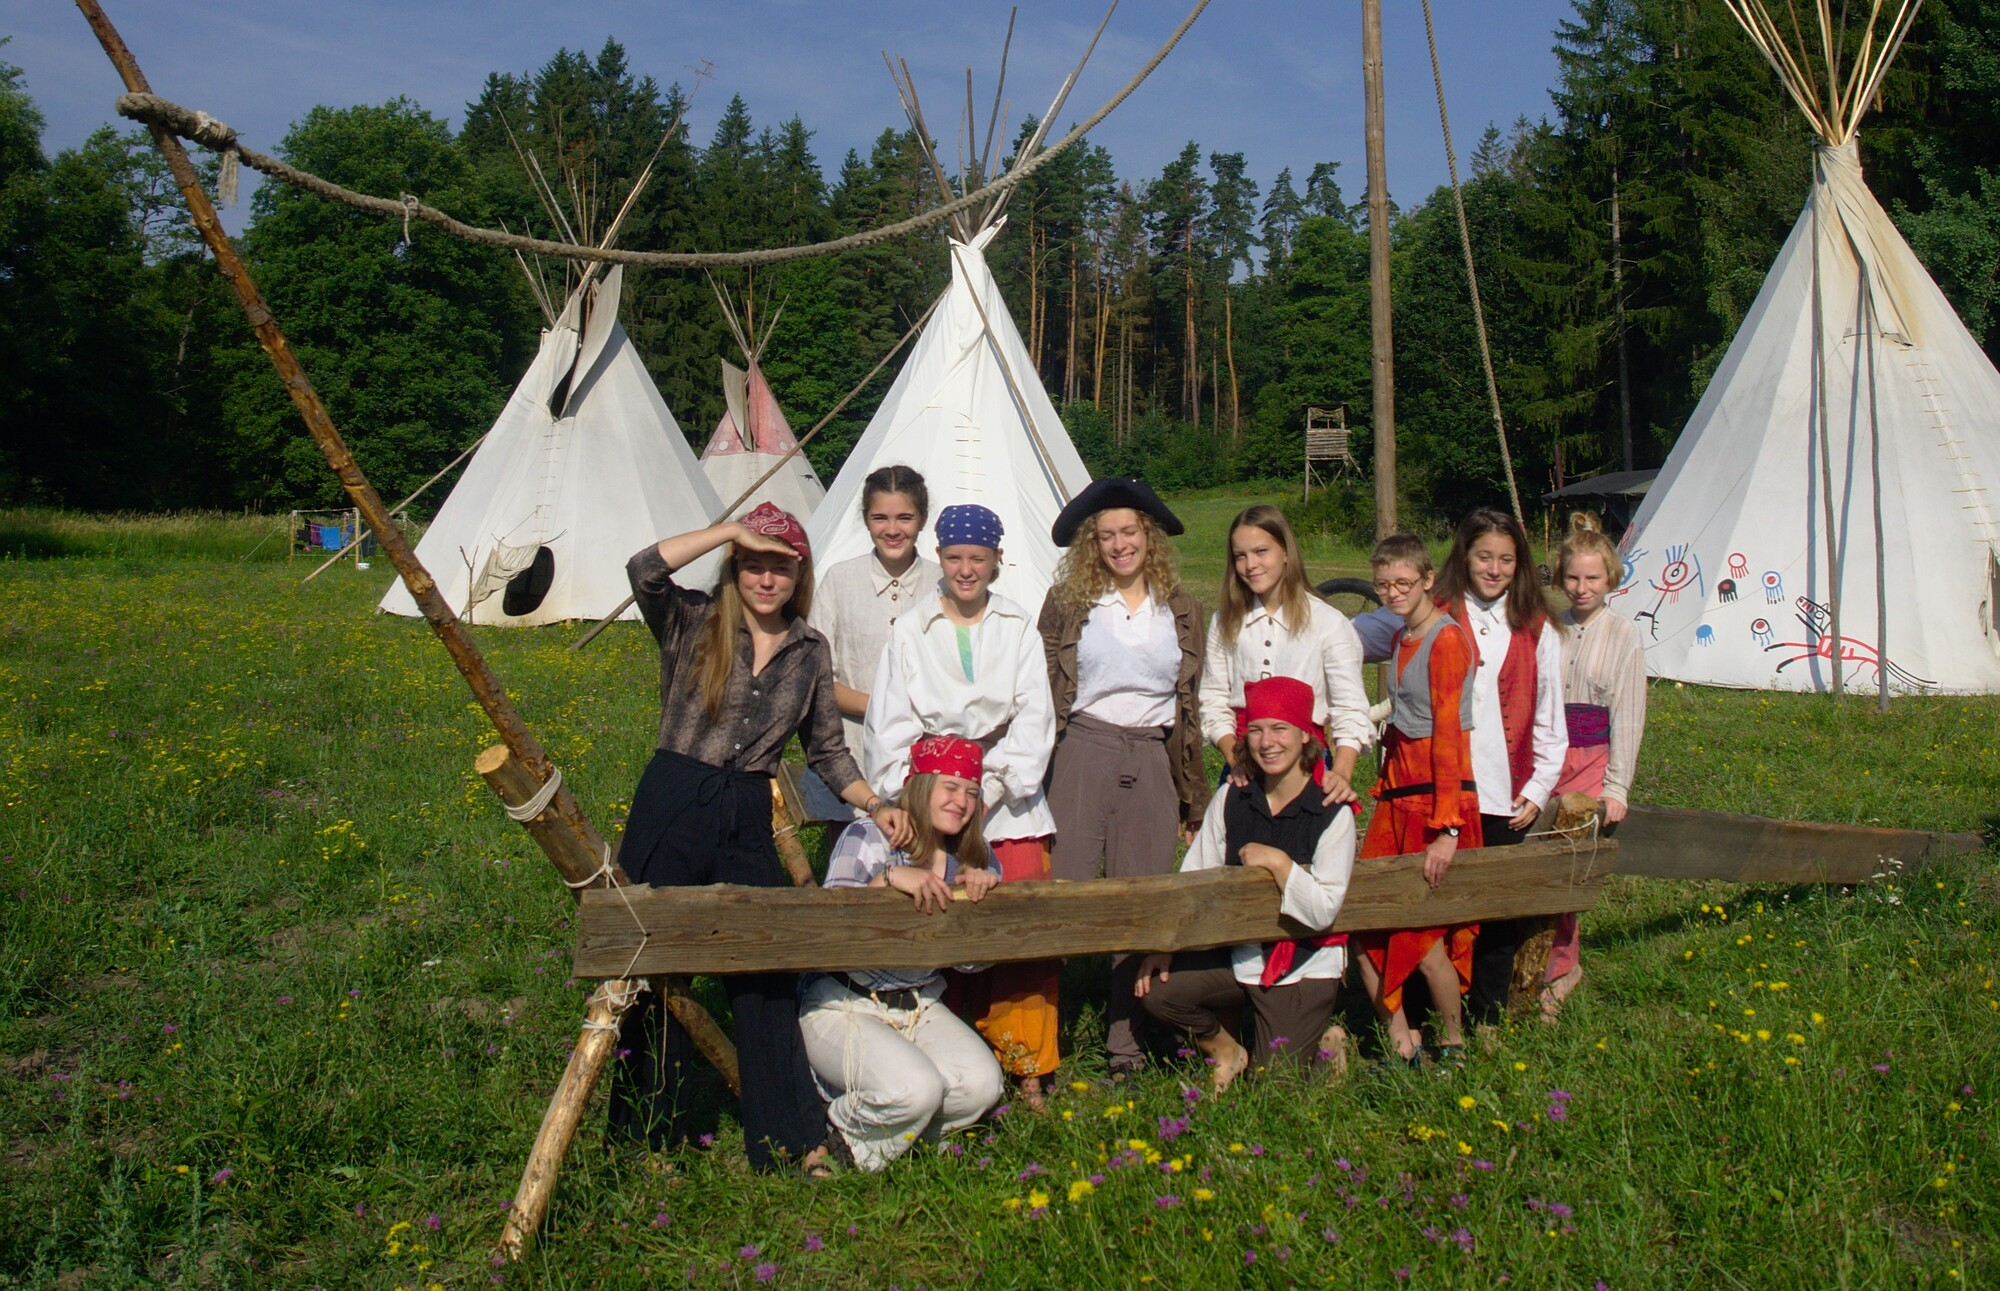
\includegraphics[width=10cm]{img/druziny/jesterky.jpg}

\end{center}


% subsection ještěrky (end)


\clearpage
% chapter střípky_očima_účastníků (end)
\chapter{Mezi dítětem a vedoucím}
\label{cha:roveri}

\subsection*{Lemuří tábor}
\label{sub:lemurui_tabor}

Letos jsme my, Lemuři, v čase posledního týdne tábora podnikali své lemurské pobývání. Tábořiště bylo situováno na polootevřené louce nedaleko Mirotic u Čimelic na malebném meandrujícím potoku Lomnice. Bylo to výjimečné místo. Otevřenou polovinou louky se na nás smálo velké široké údolí s alejí mohutných topolů. Netrpěli jsme zde nedostatkem vody, netrpěli jsme…netrpěli jsme ničím. Snad jen vedro bylo sem tam odzbrojující. Vždy nám ale byl po ruce stín, tam nám bylo dobře. Krom toho skoro každý den byl plný aktivit mimotábořištních. Jednou jsme šli na výlet, jindy byl náš cíl blízký rybník, pak byla neděle a my šli do kostela.

Minulý rok Lemuři skládali roverský slib, a tím vědomě vstupovali do roverského a z dětského času vycházeli. Roverské heslo „Sloužím!“ by se mělo nést každou roverskou akcí, a tak i my byli sloužit. Byli jsme v domově seniorů s paměťovými chorobami, otloukávali vlhkou zeď na tamější faře, vyměňovali brzdové destičky u feldy.  

Náš tábor byl ohromně naplněn pohodou a k té přispívalo hned několik věcí.

Jídlo. Hodně epesňovelkolepých jídel denně nám moc vyhovovalo. Ani čas strávený nad jejich uvařením nám nebral ani trochu chutě. Ba naopak. Měli jsme ovocné knedlíky (ty trvaly obzvlášť dlouho), rýži s moc dobrým masem, kokosem, jablky, zelím… fotky vám poví vše co potřebujete vědět.   

Dalším aspektem byly každovečerní pohodičky u ohně, v sauně (tu jsme měli dvakrát a byla moooc dobrá :-) ), s kytarou i bez ní. Přes den nám mohli být útočištěm i hamaky, ze kterých jsme si vyrobili pětipatrovou palandu.  Básně a legendy se budou na toto psát po dlouhé dekády. 

\podpis{Wexlák}
\subsection*{OBROK '19 aneb LEMŠEŘÍ VÝLET NA KONOPIŠTĚ}
\label{sub:obrok19}

Už na samotný počátek byl napínavý - masivní přihlašování je vždycky otázkou rychlosti, takže jsme všichni, kdo chtěli jet na ObRok, seděli u svých počítačů/mobilů, netrpělivě odpočítávali poslední minuty a celí nervózní čekali, až se v osm večer spustí přihlašování. Samozřejmě, servery padaly a ne všichni se dostaly hned na poprvé. Naštěstí ale ještě poté byla druhá vlna přihlašování, takže jsme nakonec (přes menší komplikace v podobě nemocí, doplňování členů apod.) na akci jeli ve složení Tarzan - jako vedoucí naší skupiny, Koala, Šárka, Wexlák, Kibitz, Šerif, Natěrač, já a pak ještě další tři skauti z Tábora - Ponožka  a jeho dvě ženy :).


ObRok jako takový se konal na Konopišti nedaleko Benešova u Prahy. Už při příchodu jsme poznali, že tu jsou opravdu lidé z různých krajů - zpívající Ostravaci se nedali přeslechnout. Bohužel, počasí nám ze začátku příliš nepřálo. Pršelo, pršelo a pršelo, což nakonec mělo dopad i na celý ObRok, kdy jsme ze subkempů museli poměrně dlouhou cestou obcházet obrokový areál, abychom se vůbec dostali k pódiu a dalším stánkům, neboť původní cesta byla velmi rozbahněná. Takže jsme často na různé ceremonie, programy a koncerty chodili později, než bychom si přáli.

\begin{center}
	
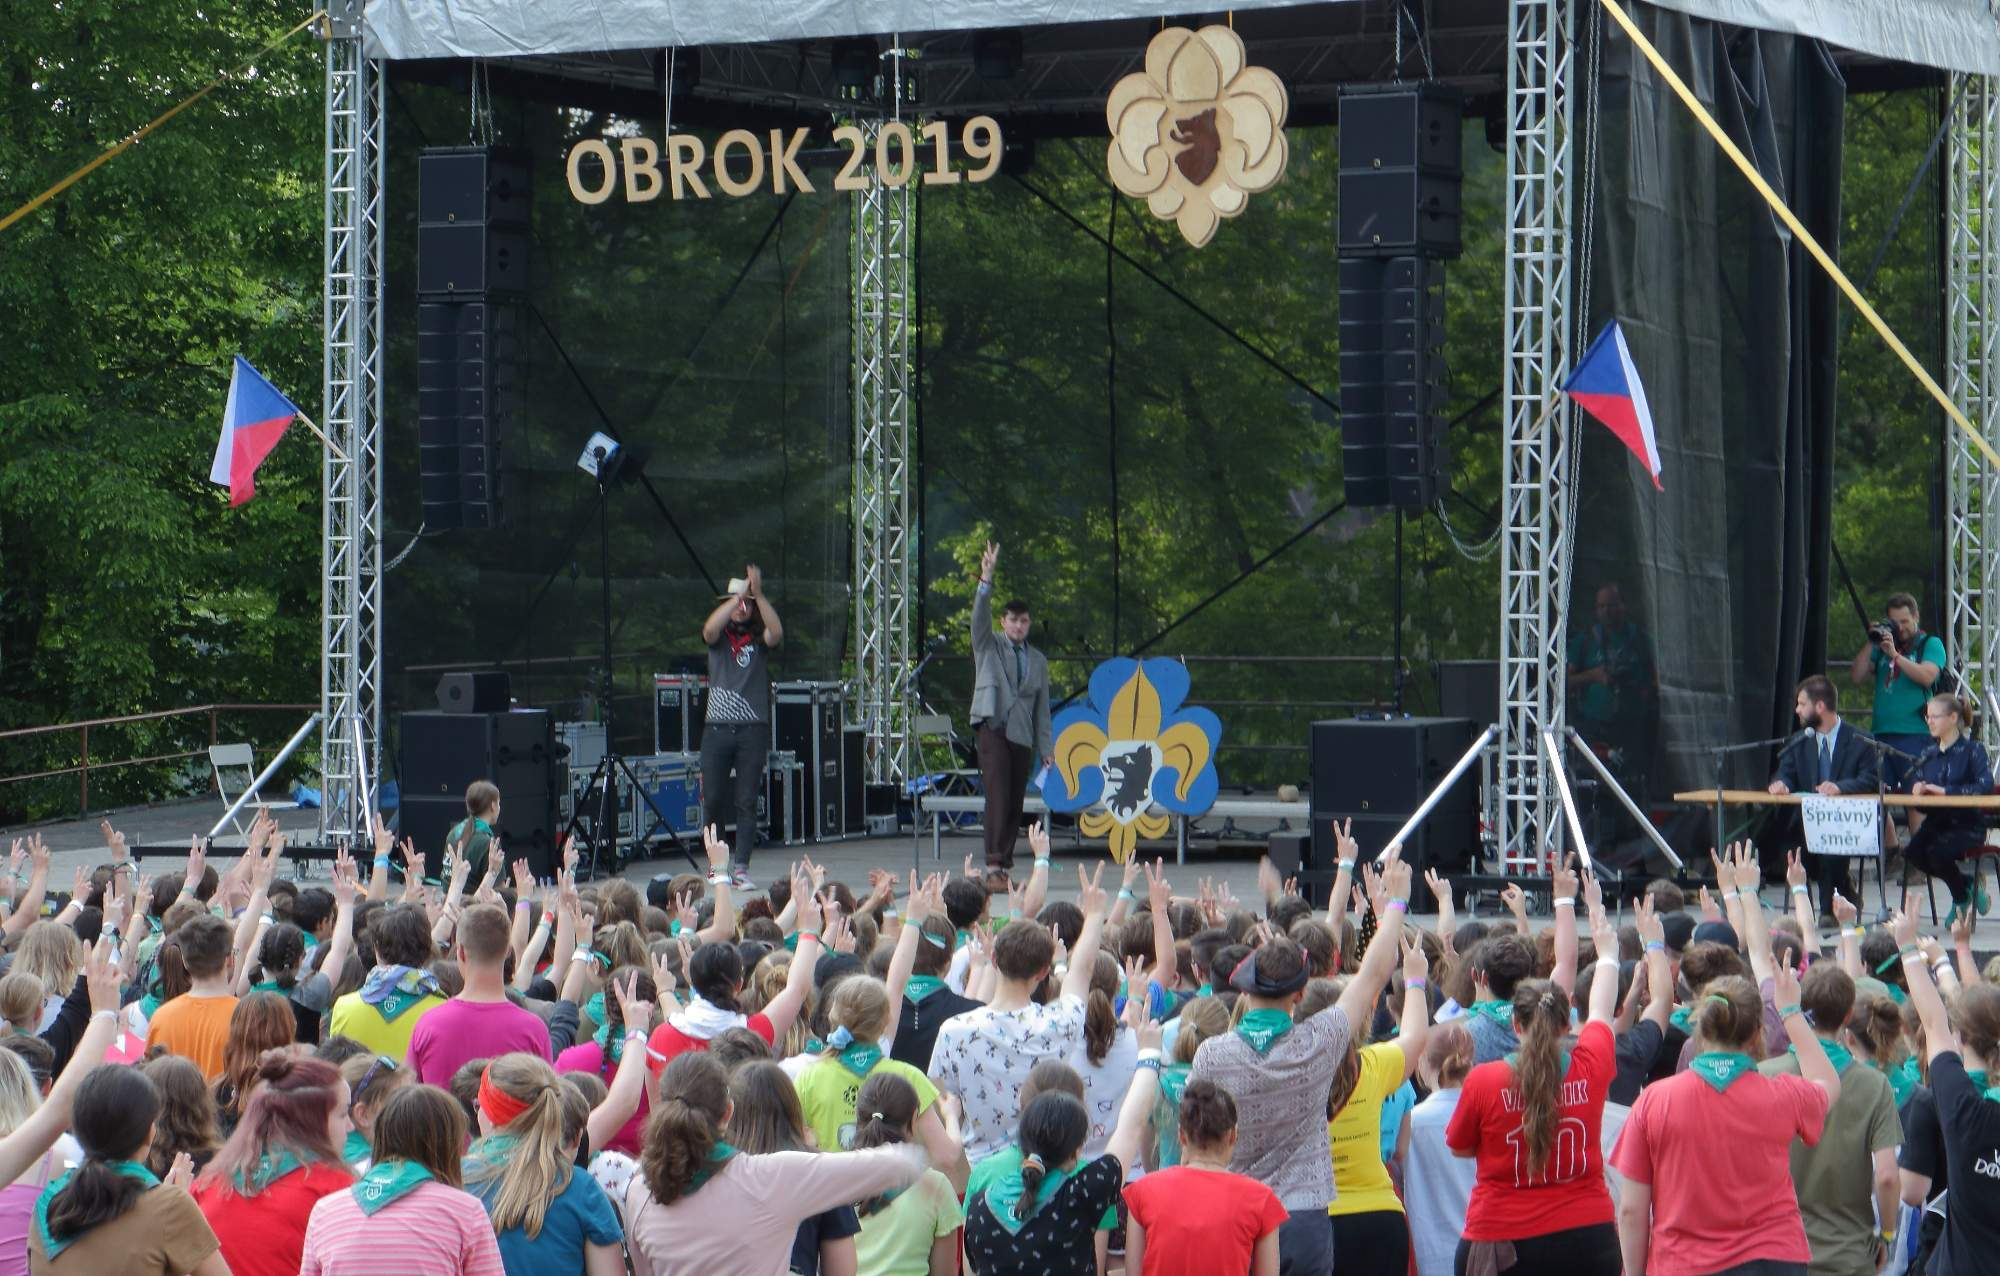
\includegraphics[width=12cm]{img/rovero_clanky/obrok1.JPG}
\end{center}

Programů tam bylo požehnaně - různé workshopy, služby, velká hra, koncerty, netradiční sporty, přednášky… člověk se tam opravdu nenudil. Ovšem vzhledem k té obrovské mase lidí bylo kolikrát těžké se někam dostat. Mě osobně nejvíce bavilo sobotní odpoledne, kdy jsme šli službit jako pomocníci při dětském dopravním dni pro benešovské. Byla jsem tam s moc fajn lidmi a potkala jsem spoustu jak roztomilých, tak vtipných dětí. Celkově zajímavá zkušenost. A samozřejmě jsem si užila koncerty (kapela Skaunk a frontman kapely Mech budiž navždy uchováni v mém srdíčku)!
Také mě pobavilo hromadné koukání na hokej v kantýně. Protože i když byl člověk na druhém konci areálu, poznal, že Češi dali puk.


Co se týče jídla, tak to se mnou bylo docela problematické. Kvůli různým problémům mi bylo od doktorky nakázáno nepožívat lepek a laktózu, takže původně velmi solidní výběr potravin se drasticky snížil na luštěniny, ovoce, zeleninu, rýži a maso. Takže si to se mnou vařící Přííšery jistě užily :). Tak či tak jsme ale vykouzlily moc dobré menu.


Jeden pro mě z mála nepříjemných okamžiků, jež se na ObRoku staly, se přihodil při velké obrokové hře - kolínko šlo do háje, což jemně zkomplikovalo náš odjezd. Díky mně jsme totiž kráčeli celkem pomalu a připočítáme-li ještě zapomenutý kotlík a České dráhy, výsledkem byla další společná a krásně strávená chvíle - čekání na vlak. Naštěstí jsme se ale všichni dostali domů relativně včas.


Závěrem bych celou akci zhodnotila pozitivně. Sice jsem si tam nenašla moc nových kamarádů, ale za to jsem si to užila s těmi starými! A věřím, že ostatní Lemšery taky!


\begin{center}

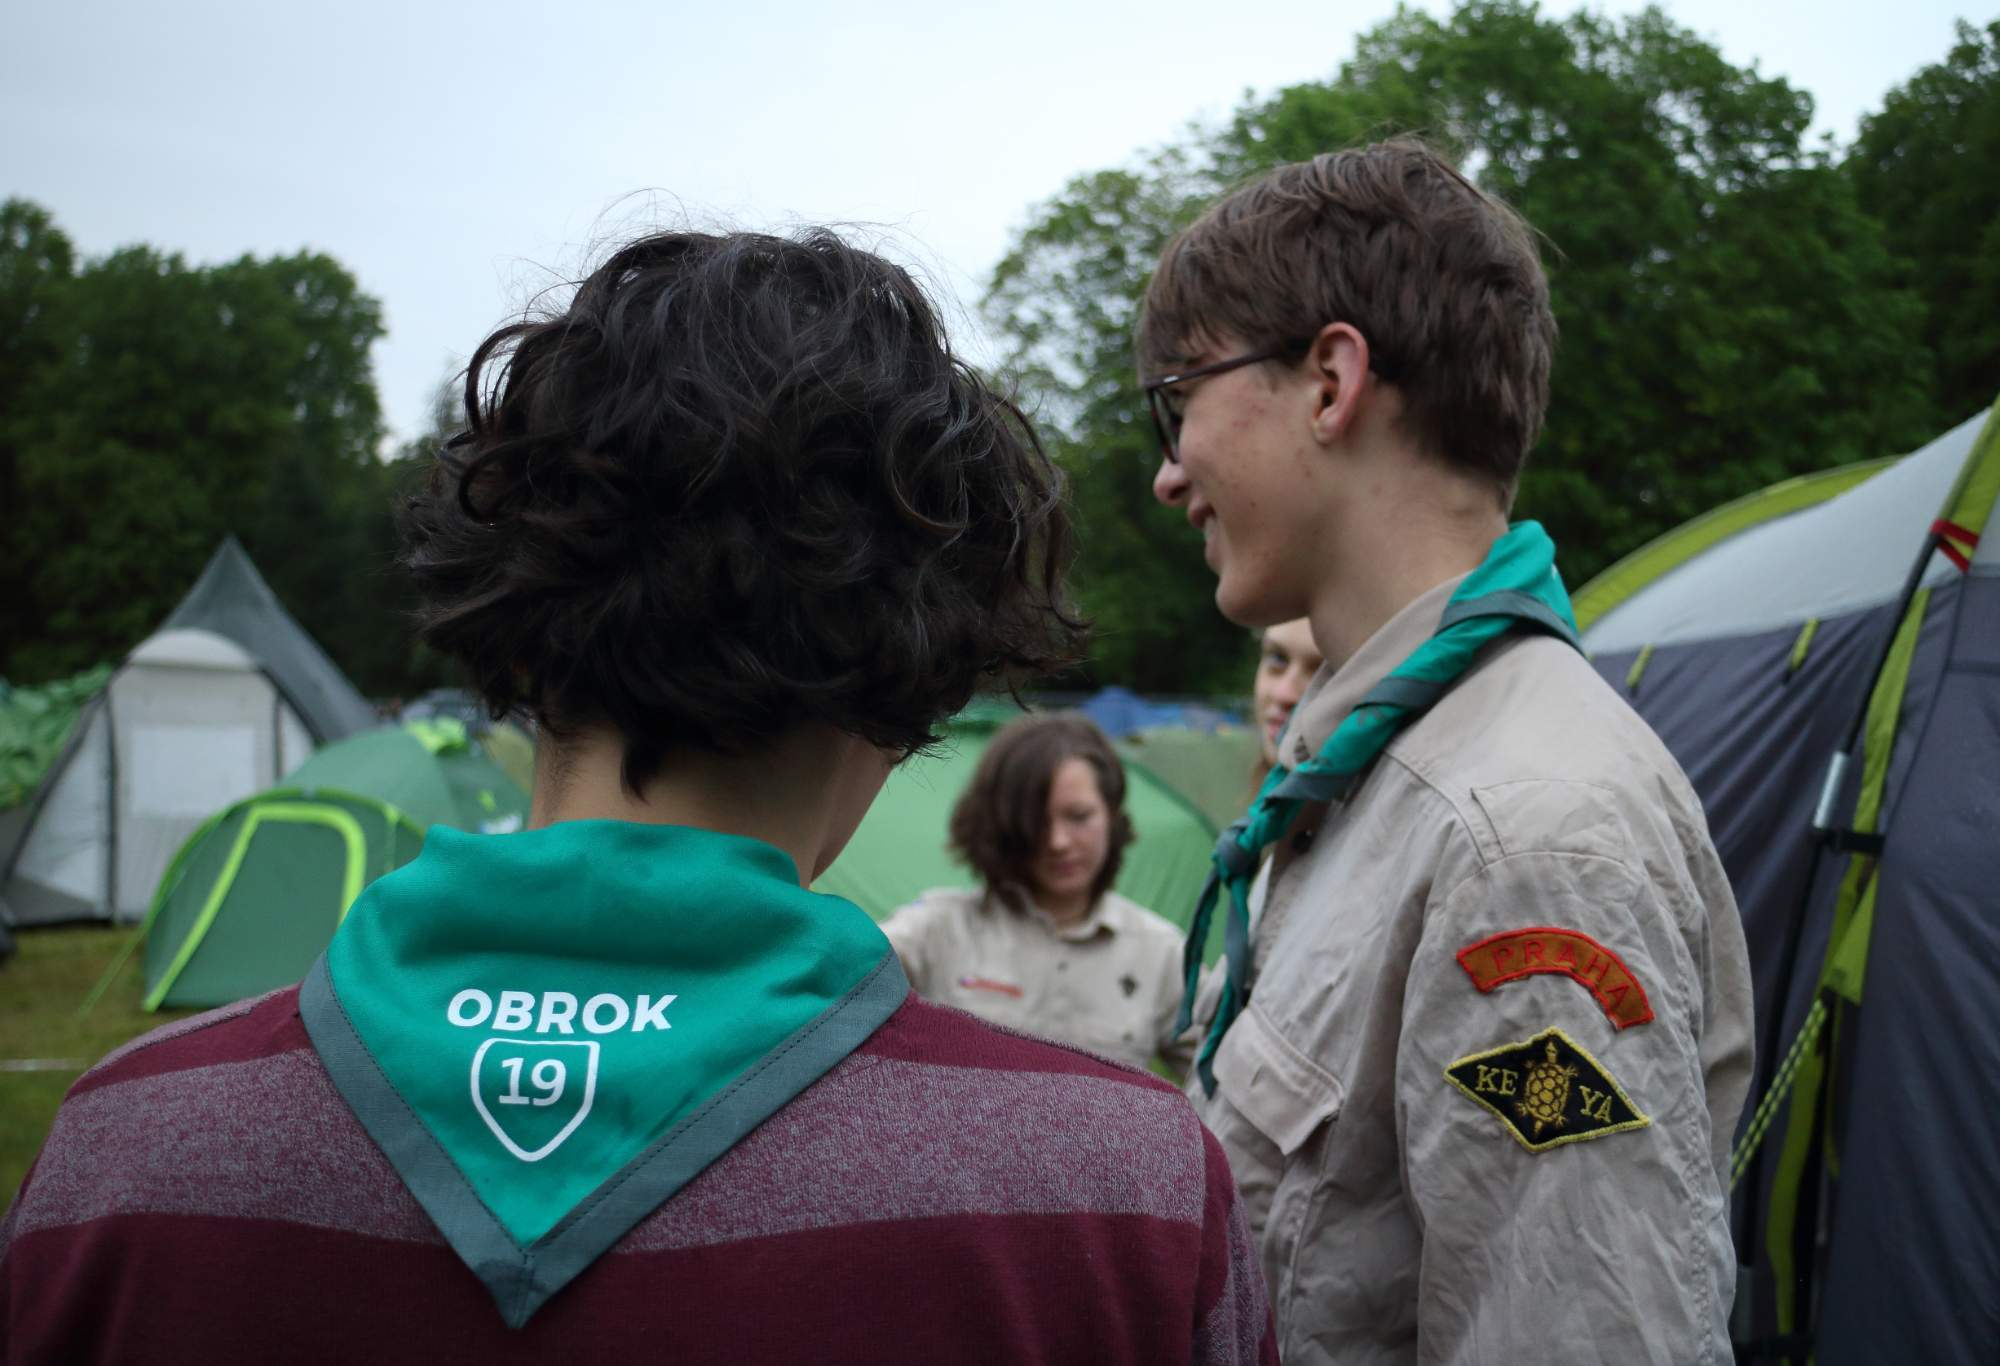
\includegraphics[width=12cm]{img/rovero_clanky/obrok2.JPG}

\end{center}


\podpis{Štípadlo}
\subsection*{Nezapomenutelná návštěva}
\label{sub:nezapomenutelna_navsteva}

V rámci Lemuřího tábora jsme se krom příjemného pobývání v lůnu přírody, debužírování na našich gastronomických výtvorech a podnikání všelijakých skopičin snažili páchat i nějaké to dobro. Ostatně roverské heslo „sloužím“ nás k tomu přímo vybízelo. Proto když jsme zjistili, že v dochozí vzdálenosti od našeho tábořiště se nachází Domov Rakovice, místo pro široké spektrum lidí stižených některou z forem demence, neváhali jsme ani na moment a jali se navazovat s tímto ústavem kontakt. To se ukázalo být nečekaně komplikovanou procedurou. Na základě telefonického hovoru se slečnou sekretářkou se mi podařilo dohodnout schůzku s paní ředitelkou, což byla žena jako vystřižená z dámského časopisu a se svými vysokými podpatky, dlouhými nehty a parfémy zvučných značek tvořila až úsměvný protiklad k mému nemytému já.
To, co se mi prve jevilo jako prostý úkol – tedy vysvětlit, že jsme skauti, co chtějí přijít a povídat si se seniory, zahrát jim písničky a prostě tak nějak pobýt – se ukázalo být úkolem nečekaně náročným. Paní ředitelka nechápala, proč bychom to chtěli dělat, jaké jsme si pro ně připravili představení a kolik za to chceme peněz. Nicméně po vyjasnění, že to děláme pro radost, že s tím už nějaké zkušenosti máme, že nemáme představení, akorát ukulele, a že za to vážně nic nechceme, šokovaná paní ředitelka nabídku přijala pod jedinou podmínkou, a to že nám budou moci uvařit oběd. Proti tomu jsme nic neměli, pročež jsme se dohodli a o dva dny později do Rakovic ošátkováni dorazili.

Kromě vydatného oběda na nás čekaly dvě skupiny klientů, kterým jsme s velikým úspěchem hráli hitovky typu Hlídač krav, Lachtani nebo Nosorožec. Po dvou „koncertech“ jsme se rozdělili do menších skupinek a jali se věnovat klientům individuálně. Někteří z nás si jenom povídali, jiní hráli stolní hry nebo dělali ruční práce, a část z nás jela provézt výpravu vozíčkářů po vesnici. Asi nemá smysl zabíhat do přílišných podrobností, nicméně z celé návštěvy jsme odcházeli s neuvěřitelně pozitivním dojmem, protože klienti i personál byli extrémně přátelští a všechno se neslo v úžasně příjemném duchu. Holt jenom někde vzadu v mozku člověku hlodal pocit smutku, protože životní příběhy klientů byly často tragické, a zejména u (překvapivě velké) skupiny s alkoholovou demencí i docela výstražné.

No nakonec jsme v Rakovicích strávili celé odpoledne. Paní ředitelka nám přes protesty vtiskla do rukou bednu čokolády a peníze na zmrzlinu a hlavně vysvětlila, proč byli všichni z naší návštěvy tak zaskočení (a proč se naše úvodní domluva nesla v duchu nepochopení) – prý se jim ještě nikdy nestalo, že by za nimi do Domova přišel jen tak někdo na návštěvu…


\begin{center}

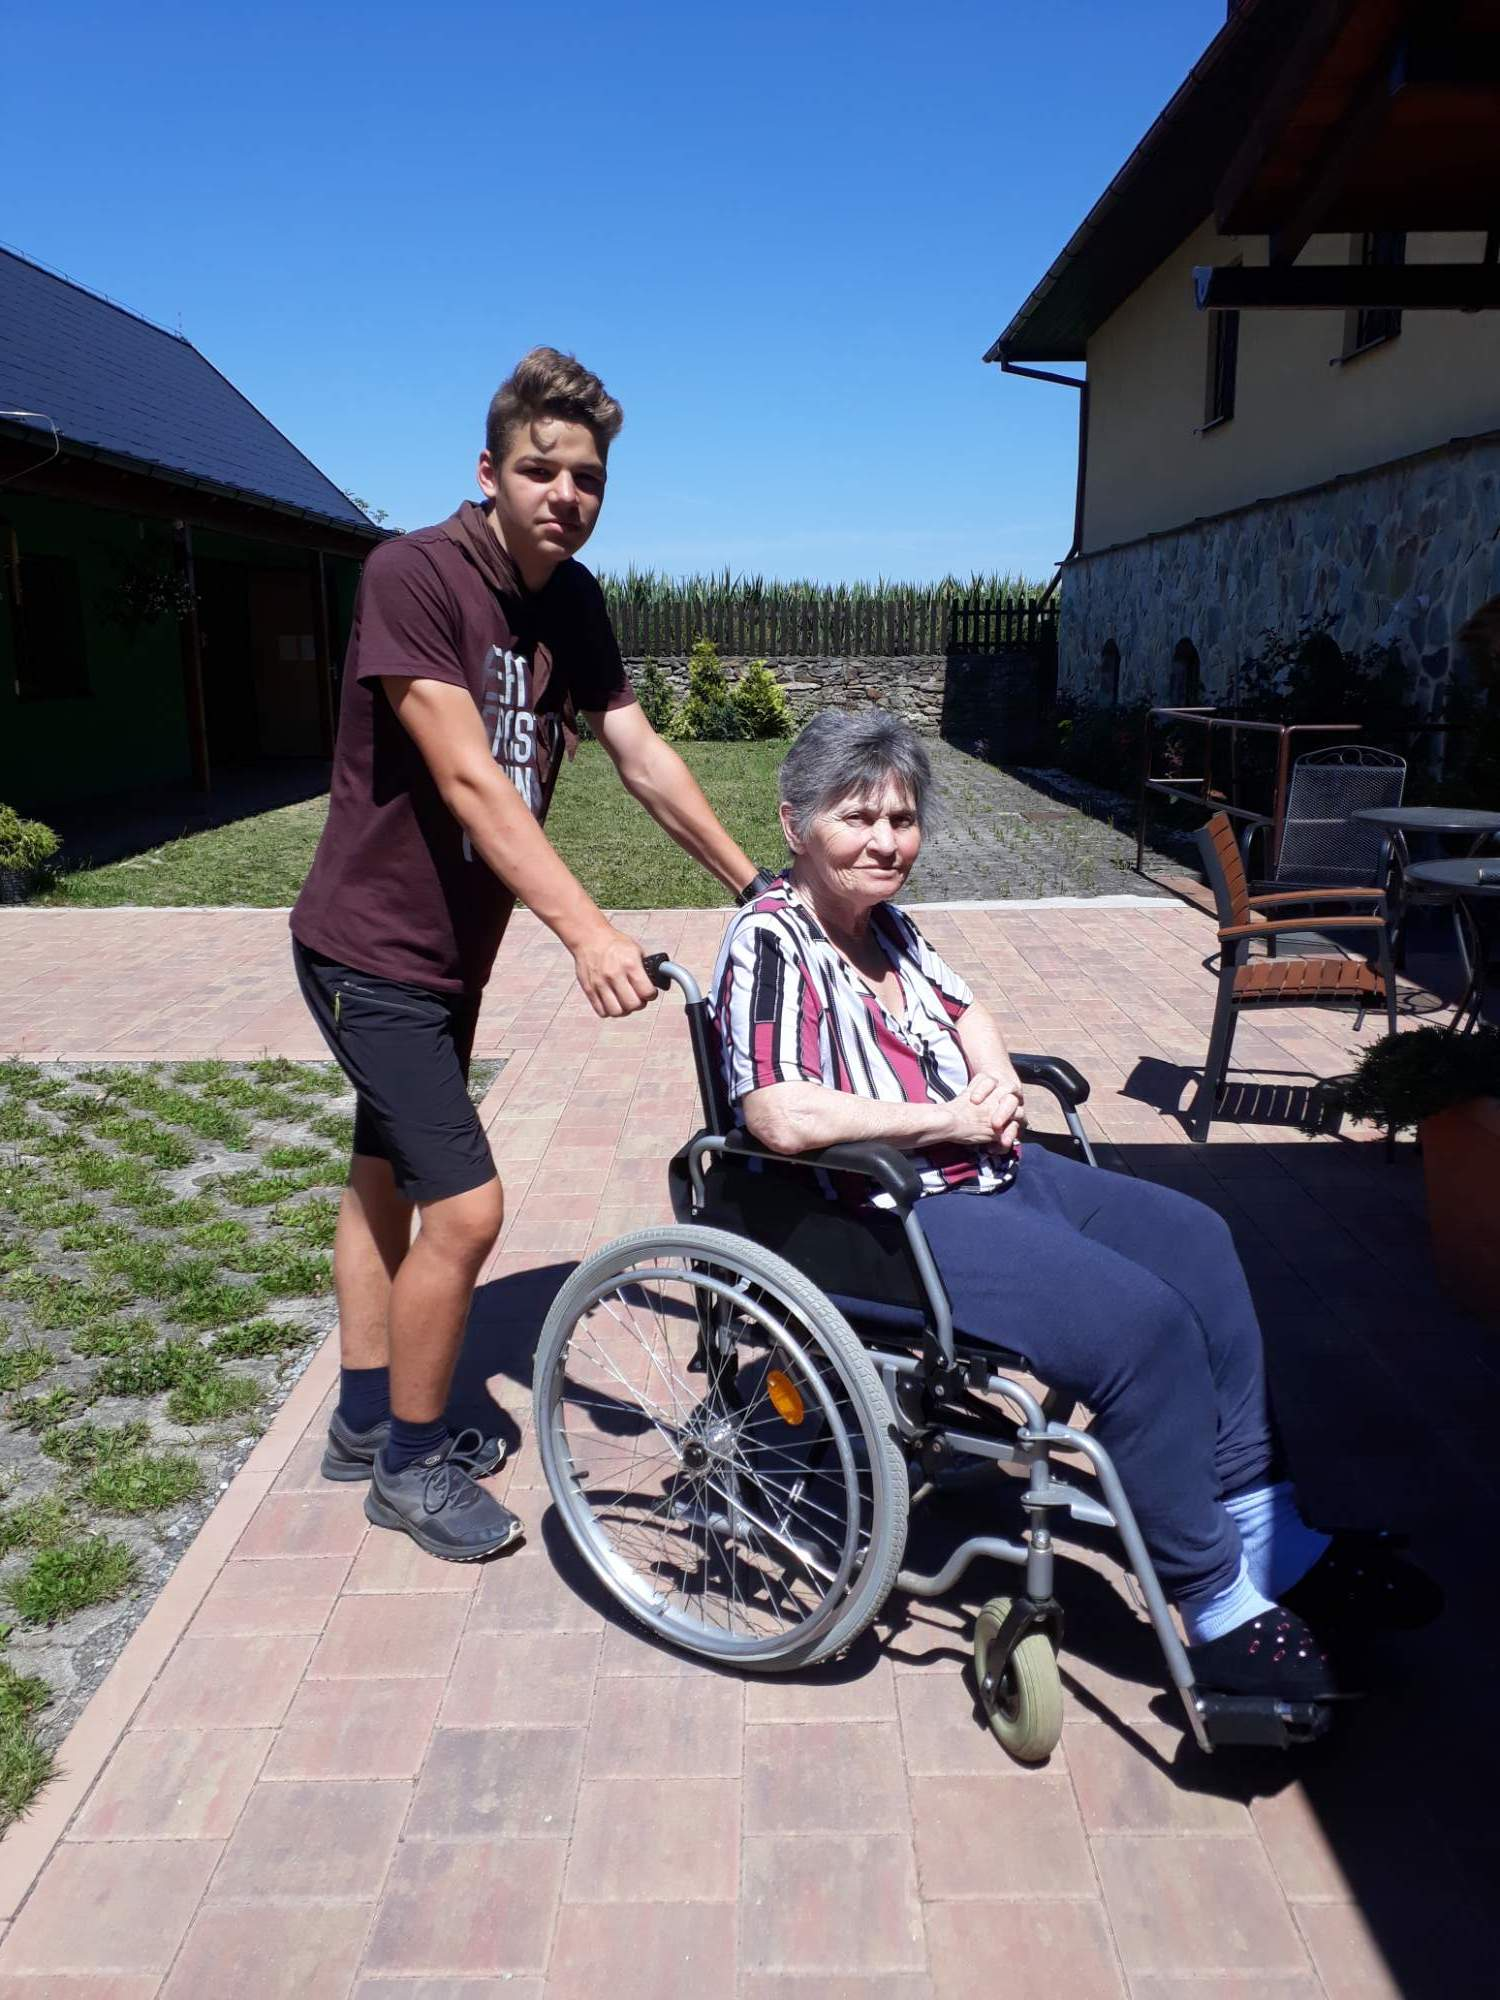
\includegraphics[width=5cm]{img/rovero_clanky/rizek_s_babou.jpg}

\end{center}

\podpis{Fík}

\clearpage
\chapter{Oddíl a tábor očima uďů} % (fold)
\label{cha:udove}

\subsection*{Jak se vaří na táboře} % (fold)
\label{sub:jak_se_vaří_na_táboře}

% subsection jak_se_vaří_na_táboře (end)

Opuchlé oči od kouře, pořezané prsty, ranní vstávání a neustálé počítání, odhadování nebo používání metody pokus – omyl. Ano, zasvěcení už tuší, tohle bude článek o táborové kuchyni.

Co vám budu povídat, vaření může být zábava, ale po třech týdnech živení spousty malých hladových krků (a pár uďovských) už máte na zbytek roku kuchtění dost. Pro vás, kteří stále netuší, co takové šéfování táborové kuchyni obnáší, mám shrnutí těch nejzajímavějších zážitků. 


Mezi těmi nejlepšími určitě nesmí chybět smažení řízků na závěrečnou popokladovkovou hostinu. Až si jednou řeknete, že udělat dětem radost touhle dobrotou je super nápad, tak vás musím varovat, není. Už jenom odhadnout počet řízků a nakoupit je byla celkem výzva a co teprve samotné krájení, obalování a smažení. Stojíte u hrnce, praží do vás současně sluníčko a oheň z kamen, pot z vás jen leje, jste popálení od prskajícího oleje a po první várce už musíte předat štafetu někomu jinému. Po pěti hodinách máte konečně hotovo všech 170 řízků a říkáte si, jestli to vůbec stálo za to. Třešničkou na dortu pak bylo zjištění, že by nám jich stačila tak polovina. Ale což, na uďovině přišly také vhod a hlavně že děti měly radost, ne?

Za zmínku stojí i připravování anglické snídaně. To jsme měly s Pískletem další skvělý nápad, jak náš jídelníček trochu ozvláštnit, a kdyby si Pískle neupustila sekeru na hlavu a nebyla na pár dní lehce indisponovaná, určitě by to byla velmi kvalitní ranní párty. Takhle to sice taky byla párty, ale pro příště asi zůstaneme u klasického poridge. Ono po ránu se snažit vymyslet, jak osmažit na našich kamnech slaninu nebo opéct tousty není úplně jednoduché a zapojit do toho skupinku službících Urzonů už je vyloženě stresující.

Nejvtipnější okamžik zcela jistě nastal ve chvíli, kdy jsme napsaly do seznamu nákupu, netušíc nic zlého, celer do polívky. Ani ve snu by nás nenapadlo takovou položku nějak víc zkonkretizovat, popsat, připojit obrázek nebo jinak upřesnit. Namísto klasické celerové bulvy se nám však z nákupu vrátily pouze celerové listy a popravdě trvalo velmi dlouho, než jsme pochopily, co že to má být. Po dlouhém a lehce hysterickém smíchu jsme „celer“ odložily do sklípku s tím, že se snad pro něj najde nějaké využití (nenašlo). 

\begin{center}

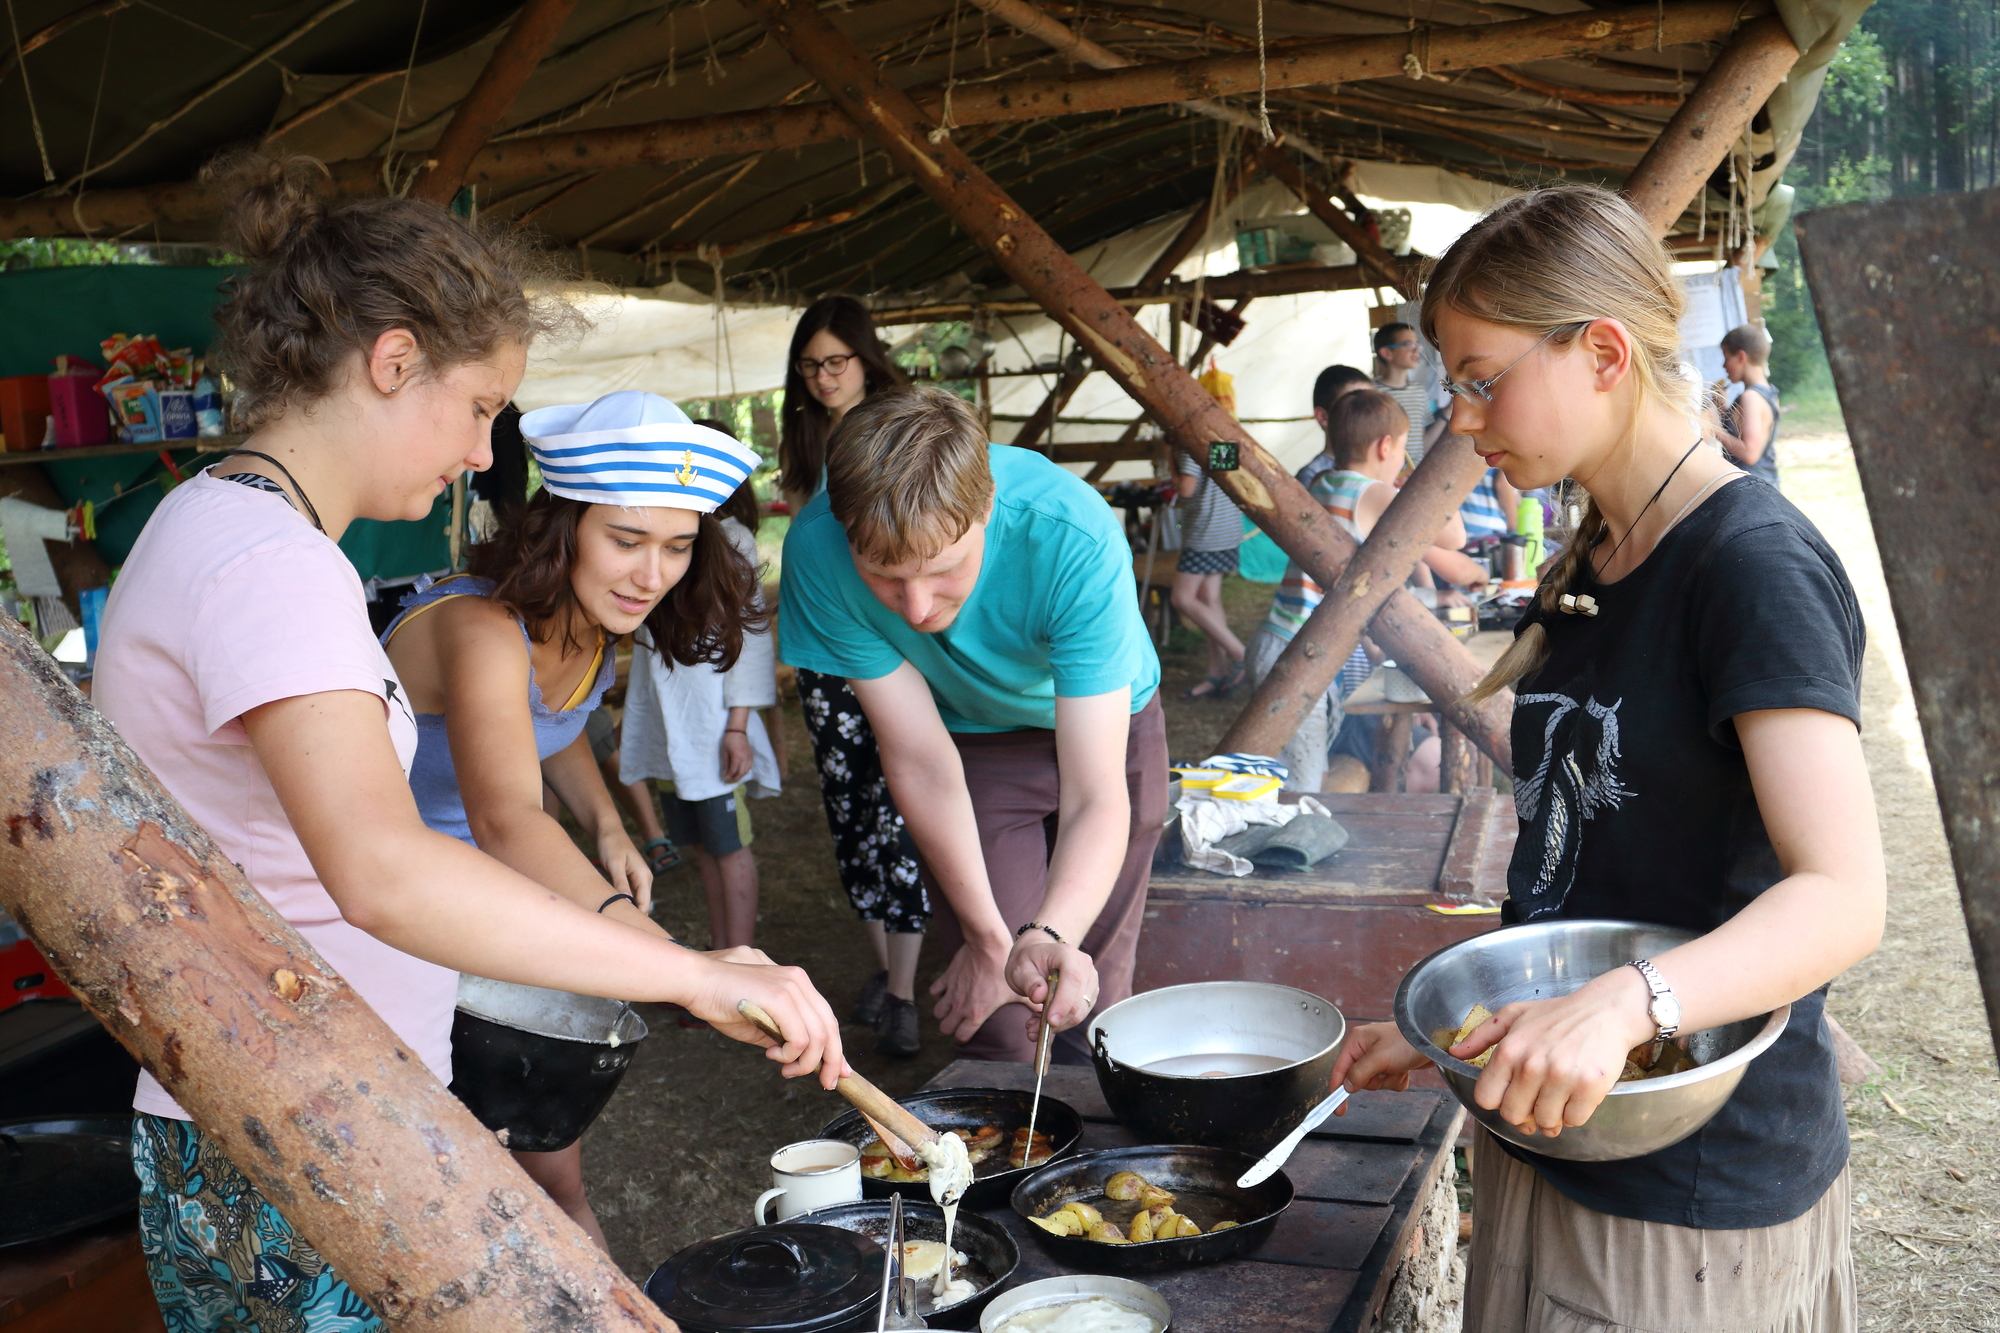
\includegraphics[width=10cm]{img/udo_clanky/kuchyne1.JPG}

\end{center}



Táborová kuchyně skýtá mnoho možností zažít věci, které si budete pamatovat po zbytek života. Jak jsme jedli celý den jenom zeleninu, jak nám myši spapaly svačinu nebo rozsekávání melounu mačetou jako nindža (přitom se mimochodem skvěle vybíjí jakákoliv frustrace). Klidně bych zvládla popsat střípky z kuchyně celou Knihu Keya, ale nechme tu prostor i pro další. Důležité je, že se zatím nikdo nepřiotrávil a všichni naše gastronomické výtvory ve zdraví přežili. 
\podpis{Kometa}


\subsection*{Převoz tyčí aneb reklama na Boba}
\label{sub:převoz_tyčí_aneb_reklama_na_Boba}

Zajištění tábora je po všech stránkách zajímavá a občas dost náročná záležitost, která se skládá z mnoha dílčích úkolů. Patří mezi ně hledání tábořiště, obvolávání a navštěvování vlastníků, plánování programů a mnoho dalších nutností. Jak už z názvu vyplývá, rád bych vám představil letošní úspěšný převoz.

Vše začíná na Kačerově, kde se scházíme v pátek v podvečer. Vyrážíme ve složení já(Humr a auto), Hafík, Koala a Terka . Dohoda s Bobem zní, že se potkáme s jeho tranzitem na kopci nad tábořištěm Hanyetu u Syrova. Vzhledem k očekávané situaci na dálnici (zprávami zrovna běžely hrůzné zkazky o ucpané D1) se rozhodujeme pro cestu přes Benešov a Vlašim. Cesta z Prahy, která by normálně měla trvat okolo 1 hodiny po dálnici se tak měla o půlhodinky prodloužit. Nápad jet přes Benešov má bohužel víc lidí, takže nakonec dorážíme na místo s 1,5hodinovým zpožděním. Bob se prozíravě rozhodl ignorovat fake news a přijíždí i s vozejkem po dálnici, takže si stíhá užít pěkný západ slunce a začít s taháním týpiovek. Tyče zbyly na tábořišti po zimních týpkařích – šlo jen o jedno týpí – zbytek je uložen na pile u Jiřiček. Za večer stihneme jakž takž vytahat tyče nahoru k autu – kopec bychom nevyjeli – a utábořit se na louce u Jiřiček. Večer se vyrábí večeře ze všech možných zbytků, kombinace nudlí, tortill, Terčina salátu(polníček?) a konzerv je lahodná.



\begin{center}

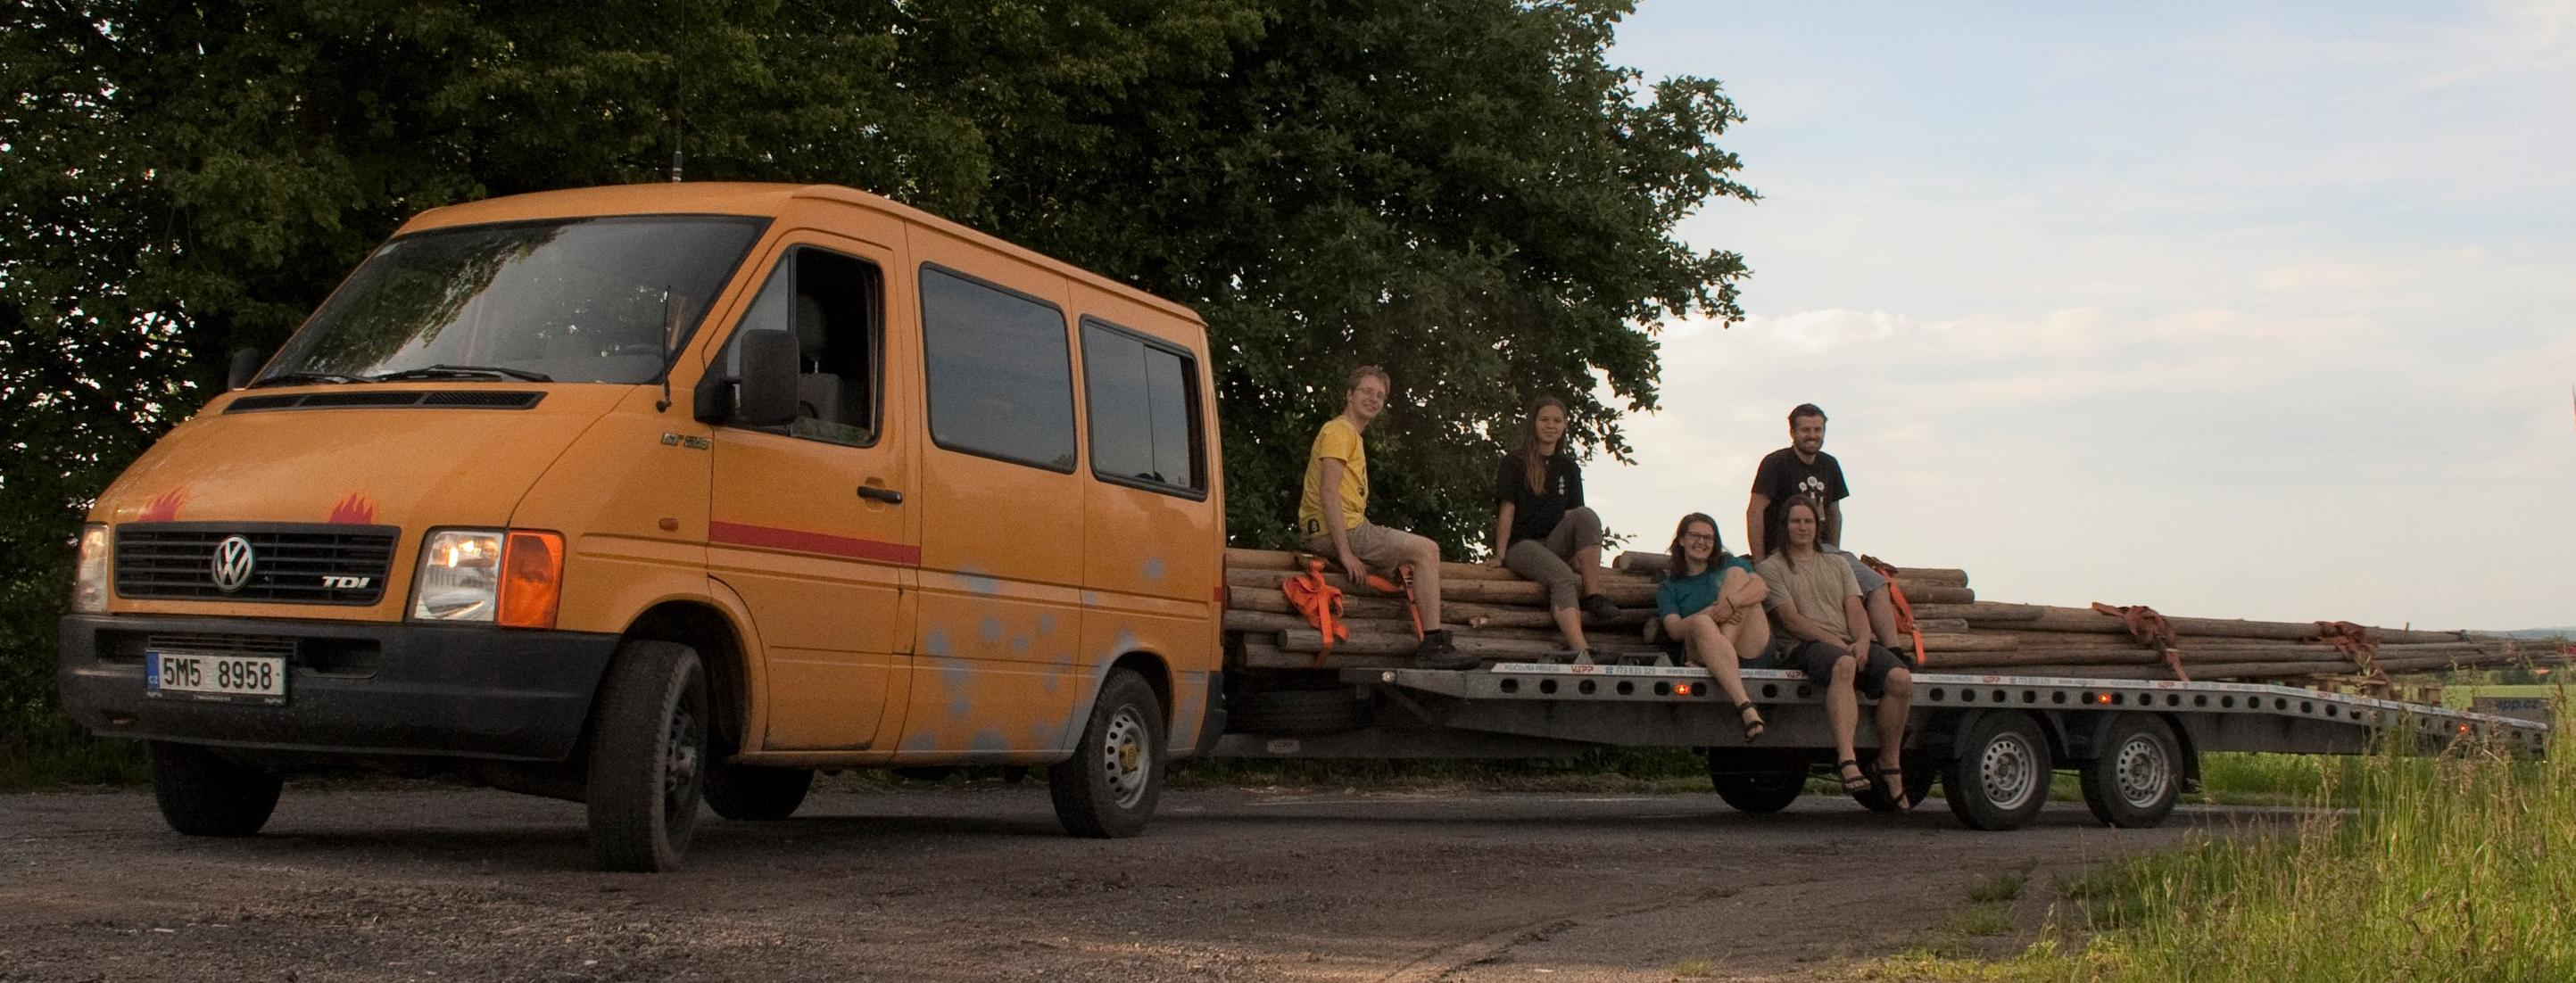
\includegraphics[width=12cm]{img/udo_clanky/Prevoz_tyci_2019_010.jpg}
\end{center}

Vstáváme brzy, abychom začali co nejdříve, čeká nás totiž převoz asi 150 kousků do 100 kilometrů vzdálené Vráže. Dle map bude cesta trvat 1,5 hodiny a nejsme si jisti, kolik tyčí zvládneme převézt v jedné várce. Každopádně, doufáme, že se nám podaří vše odvézt během dne, abychom byli večer doma (bláhové?).

Tyčí je mnoho, počítání náročné, 1.várka nám zabrala asi hodinu a čouhá metr a půl přes vozejk (většina tyčí má okolo 9m a více), snad tomu aspoň trochu pomůže červený praporek. Jedou obě vozidla – já s Koalou a Hafíkem se stavíme koupit oběd a potenciální večeři, a Bob s Terkou míří rovnou na tábořiště. Sraz máme ve Vráži u kapličky, s obědem i lahodnými zbytky od večeře čekáme na tyče. Voláme s tranzitem a zjišťujeme, že to vzali přes vesnici, ze které nevede most na druhý břeh Vltavy a teď musí vycouvat zpět na hlavní silnici. Nakonec doráží s mírným zpožděním, vykládáme tyče, necháváme doprovodné vozidlo ve Vráži a jedeme si pro další várku. Cestu si krátíme přednáškami z historie, recitací klasické arabské poezie, vyprávěním příběhů z dávných dob uďovství a debatováním o tématech, které si už nepamatuji, ale pamatuji si, že se o nich velmi živě debatovalo… Jo, a je pekelné vedro. 

Druhá várka nám jde od ruky a vypadá to, že bude náš tyčový park naložen, ale nakonec ještě asi 30 tyčí zbude. Pár tyčí pro jistotu seřízneme, naobědváme se a hurá směr Vráž. Témata pomalu dochází, spánek přichází. Bob naštěstí nespí a řídí. Poslední várku už nějak dotlačíme na vozík, vyfotíme se a odvezeme se. Jsme všichni mrtví a nechápeme, že Bob ještě zvládá řídit. Nu, je to Bob. Končíme v půl osmé po 12 hodinách převážení, nakládání a vykládání. Jdeme se ještě projít po Anpetu tábořišti, kde je všude vysoká tráva, takže se následně vracíme řádně oklíšťováni.
Nakonec nás čeká cesta do Prahy, během které posloucháme klasickou hudbu. 

Během převozu bylo celkem spáleno 90,3 litrů nafty a ujeto 832 km = průměrná spotřeba 10,85l/100km. Statistika namožených svalů a rozsezených zadků není k dispozici.

\podpis{Humr}



\subsection*{Nejlepší uďovský zážitek na táboře}
\label{sub:nejlepší_uďovský_zážitek_na_táboře}

Bohužel tento text vzniká přesně 131 dní po konci tábora, což znamená, že zážitky již v paměti nejsou tak živé. Nicméně, sepíšu alespoň sled výrazných událostí, které mě na táboře ovlivnily, a které přece jen ještě v paměti zůstávají.

Nakládáme materiál pro oba tábory náhodně do tranzitů, celý tábor si vozíme věci z jednoho tábořiště do druhého, Příšery si postupně kopají bazény v lese místo later(je tam fakt hodně vody), Urzoni jsou na stavebce, stavíme týpko na 4x, Špuntí šmouloprogram má úspěch, koupeme se o půlnoci v rybníce, král pirátů byl oběšen, Pískleti spadla sekera na hlavu, oholil jsem si vousy a nechal si jen velmi slušivý knír, dostali jsme kurděje a celý den se jí jen zelenina, Urzoni propíchli týpko chlopňovkou, Kámen kamení, během manévrů jachtíme v bezvětří na Orlíku, pozorujeme hvězdy, Jula přepadá tábor, Míček naučila papouška Kukumbrie novým hláškám, přeučujeme papouška na jiné hlášky, není sauna, Karkulka si zabodla dřevo do nohy, jedeme se koupat do Vltavy, holky smaží šílené množství řízků, poslední 2 dny tábora jíme jen řízky, šílené balení/vybalování a návrat z tábora, v Praze je maraton. 

\begin{center}

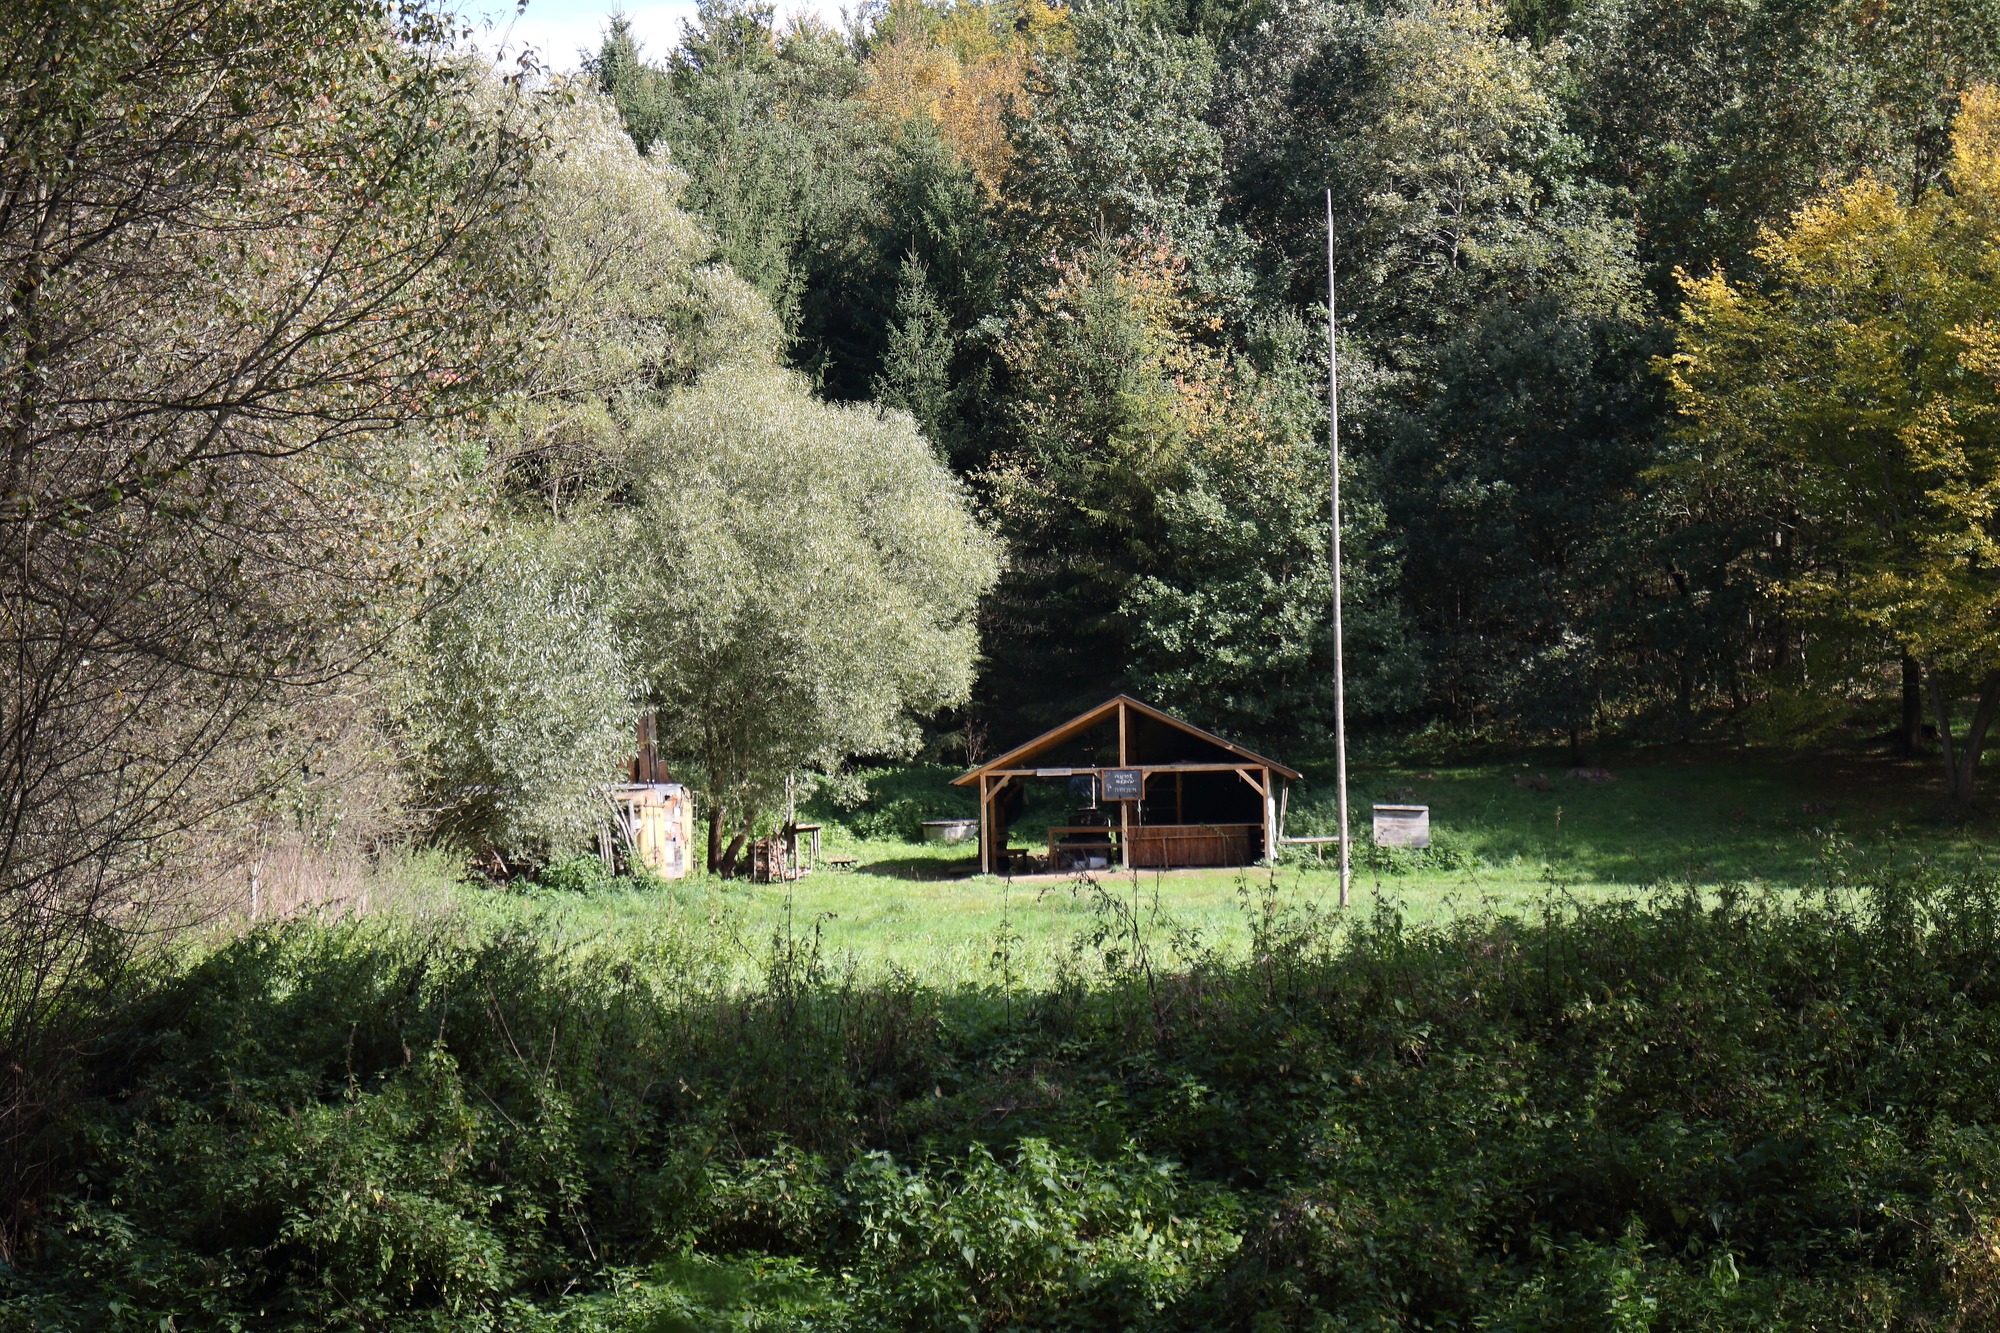
\includegraphics[width=10.2cm]{img/udo_clanky/hledanitaboriste.JPG}

\end{center}

\podpis{Humr}

\clearpage

\subsection*{Nejvíc chladný zážitek z tábora} % (fold)
\label{sub:nejvíc_chladný_zážitek_z_tábora}

% subsection Nejvíc_chladný_zážitek_z_tábora (end)


Rád vzpomínám na tábor. Jako jeden z nejvíce zaznamenaní hodných momentů letošního tábora byla příhoda z jednoho hezkého večerního koupání. Já, Einstein a H-Hruška jsme se zdrželi o něco déle. Cachtali jsme se a plnili si 20 vteřin na drsňáka. Nějakým řízením osudu se stalo, že jsme si začali počítat minutu ponořeni po krk ve vodě. Pojato to bylo v duchu jazykově vzdělávacím. Po minutě počítání v němčině jsme se, aniž bychom se vynořili, jali počítat v jazyce českém. Po minutě naší mateřštiny jsme přesedlali na angličtinu, po ní následovala francouzština se svým tak typickým způsobem zmateného počítání (tu zajišťoval Einstein). Dalších jazyků jsme neuměli. Naštěstí jsme měli po ruce pomocníky. Rebelka a posléze Tatranka nám další minutu počítali španělsky. Humra se nám sice zprvu podařilo ukecat k arabštině, ale po chvilce ho to nejspíš přestalo bavit, takže odešel. Arabskou minutu jsme dopočítali tuším opět v němčině. Pak jsme se vynořili. Strášně to pálilo. Všude. Vážně. Měl jsem dojem zápalu plic, Einstein zase, že "trochu" zemřel, dle H-Hrušky to bylo prostě strašné. Nejdřív jsem se bál, že z toho nastydneme, protože jsem kašlal a sýpal, ale nakonec nám z 6 minut studeného pokoupáníčka zbyla jen hezká vzpomínka. 
\podpis{Hafík}

\subsection*{Tábor - co a jak, ale z jiné stránky ;)} % (fold)
\label{ssub:tábor_co_a_jak}


Možná že někteří tuší, někteří netuší a někteří třeba i ví. Naše Keyácké souoddílí čas od času mění tábořiště, přesněji řečeno přibližně jednou za dva roky. Nemáme totiž žádné trvalé tábořiště. A vlastně ho ani nechceme.
Přece jenom, střídání tábořišť má takové svoje kouzlo… 
Ale taky to s sebou nese mnoho práce s nalezením vhodného místa k táboření (tak, aby tam například už nebyl nějaký jiný tábor).

Pojďme se na ten tábor podívat s širšího pohledu: takhle nějak se tábor chová v průběhu roku: \\
\textbf{Září:}

Prázdniny jsou pryč a je čas všechno začít postupně řešit. Tady se vybírá úderný tým několika uďů, kteří budou mít místo k táboření pod palcem.\\
\textbf{Říjen:}

Zvolený tým se schází a začíná první fáze hledání vhodné louky. To znamená prohlížení map a satelitních snímků, hodnocení různých kritérií a následný výběr těch nejlepších luk.

Následně se svolává výjezd a pár uďů se jede na louku podívat, například zhodnotit stav potoka a lesa.\\
\textbf{Listopad:}

Výjezdy ještě pokračují. Obvykle bývají přibližně dva až čtyři v průběhu jednoho hledání tábořiště.
Když se podaří najít vhodnou louku, svolává se další porada, která má za cíl zjistit kdo louku vlastní a jestli nám tam v létě dovolí tábořit.
\begin{center}
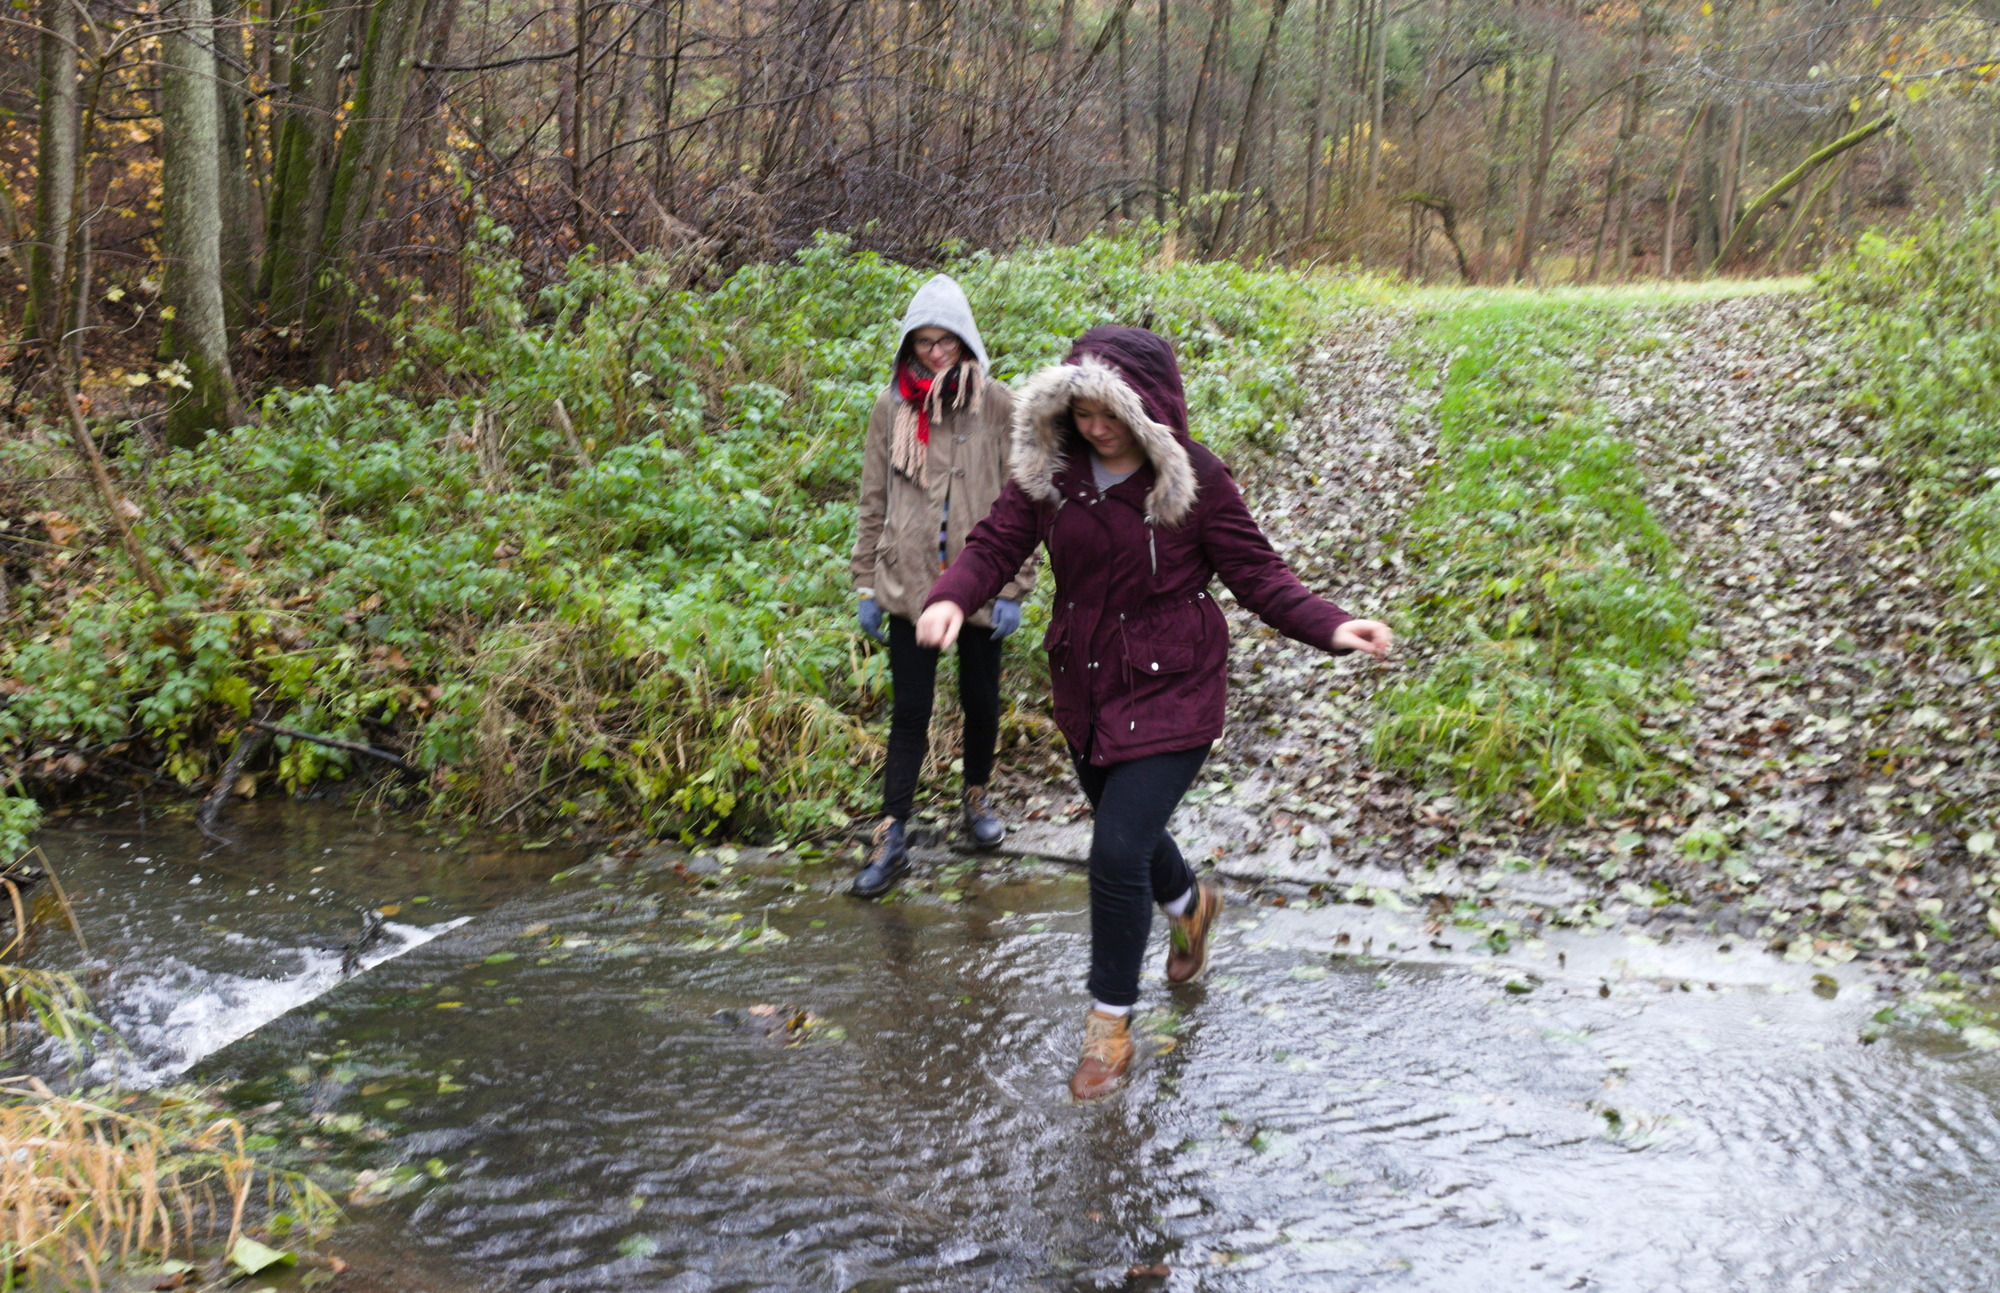
\includegraphics[width=8cm]{img/udo_clanky/hledani_brod.jpg}
\end{center}
\textbf{Prosinec:}

Ještě před novým rokem se hodí mít nalezené vhodné tábořiště a již komunikovat s majitelem. I když někdy to třeba nevyjde…\\
\textbf{Leden, Únor:}

Pokud už tábořiště máme nalezené a majitel souhlasí, je všechno v pořádku a není potřeba se příliš stresovat.\\
Pokud ale tábořiště ještě není, je problém. V takovém případě je potřeba zopakovat všechny předchozí kroky, ale rychleji a efektivněji.\\
\textbf{Březen, Duben:}

Tábor se postupně blíží a vše nabírá konkrétnější rozměry. V průběhu jara se pro jistotu ještě jednou vypraví vybraný uďotým zkontrolovat budoucí tábořiště.\\
\textbf{Květen:}

Konkrétní rozměry jsou ještě konkrétnější a začíná administrativa. Je potřeba řešit například smlouvy související s loukou a odběrem vody z nejbližší vesnice.\\
\textbf{Červen:}

Jde se k praxi a předtáborovému mazlení se se dřevem. Všechny týpiovky zůstávají obvykle na pile v blízkosti bývalého tábořiště. A teď je potřeba je dovézt na to nové. 
Obvykle to zabere jeden celý den, takže je převoz tyčí spíše dvoudenní akcička.\\
\textbf{Červenec:}

Jedeme si postavit svůj tábor, jej!
A tady už přichází vysněná odměna pro tým, který pracoval přes rok: když se na louku postaví několik týpek, hned vypadá úplně jinak.

Někdy se vydaří, a můžeme být na jedné louce dvakrát. To pak odpadá hledání, ale i tak je potřeba někdo, kdo se přes rok o tábořiště zajímá.
Například letošní tábořiště u Ostrovce nám pěkně zavařilo s potokem a pak i rybníkem. Takže pro příští rok jsme kritičtější na ostatní louky a velikost jejich potoků.

\podpis{Koala}

% subsubsection tábor_co_a_jak (end)
\subsection*{Eskymáci na táboře} % (fold)
\label{sub:eskymáci_na_táboře}

% subsection eskymáci_na_táboře (end)
Musím říct, že letos bylo přebývání s eskymáky v teepku zejména v noci o dost míň děsivý než loni. Kluci se nás před táborem ptali, jestli zas budem po uďovinách zvedat všechny eskymáky popadaný na zemi zpátky na postele. Kupodivu to letos nebylo skoro potřeba, stávalo se to opravdu výjimečně. Ani se mi nestalo, že by mě například v noci zvedala Undži z postele za ruku se slovy: ,,Pojď Debat, já Ti pomůžu", jako loni. Ale že by byla v noci úplná nuda, to se říct nedá. Například jednou jsem přišla po uďovině do teepka, kde zrovna byl Mozart a prosil mě, jestli bych mu nepomohla vzbudit Undži, protože mu to vůbec nejde. Místo Undži se ale vzbudila dřív Špageta, který jsme hned řekli, že má spát dál, že už hlídku měla a mezitím, co jsme se snažili probrat Undži, podplula Špageta pod plachtou a zmizela. Šla jsem se podívat ven a myslela jsem, že bude hned za naším teepkem, ale chvilku mi trvalo, než jsem ji v té tmě našla, protože už byla od něj dost daleko. Moc nechápu, jak se tam dostala tak rychle, vzhledem k tomu, že byla celou dobu ve spacáku. Každopádně jsem k ní šla a když jsem se ji snažila přimět k tomu, aby se vrátila do teepka, nakráčela si to k teepku Borúwčímu. Tak jsem ji nakonec vzala a Špagetku ve spacáku jsem donesla zpátky do postele. Mozart se mi smál a Špagetka o tom ráno vůbec nevěděla a smála se tomu taky velice. Takže s Eskymáky je o zábavu postaráno i v noci.

\podpis{Debat}

\subsection *{Omán - země sultána, nafty za 10 korun a pánských pyžam}
\label{sub:omán_-_země sultána_ nafty_za_10_korun_a_pánských_pyžam}

V rámci svého studia na Fildě jsem se vydal na kurz arabštiny do Ománu. Fakulta mi tak umožnila strávit 2 měsíce na Univerzitě Sultána Qábúse pro výuku arabštiny v Manahu – malé vesnici na pomezí Zelených hor a pouště. Studium na Univerzitě zní honosně, ale v Manahu je fakulta specializovaná pouze na výuku arabštiny pro studenty, jejichž rodným jazykem není arabština a tím pádem to je spíše komorní záležitost. Dohromady se nás sešlo 25 nadšenců různých věků a velikostí z celého světa – od Indonésie až po Velkou Británii. 

Nevím, co se vám vybaví, když se řekne Omán. Já každopádně před odletem myslel na vedro, velbloudy a mrakodrapy. Na konci října bylo v Praze okolo 0, Maskat (hlavní město) mě přivítal ve 2 v noci svěžími 30 stupni. Velbloudy tu vídám celkem pravidelně – kus od koleje je velbloudí farma (plot s beduínem a velbloudy) – a mrakodrapy tu nejsou, protože je SQ(sultán Qábús) zakázal – rušily by urbanistický ráz města! 

Jinak ale tato zem, původně zvaná Magan, působí úplně jinak, než jiné arabské státy.

\begin{center}
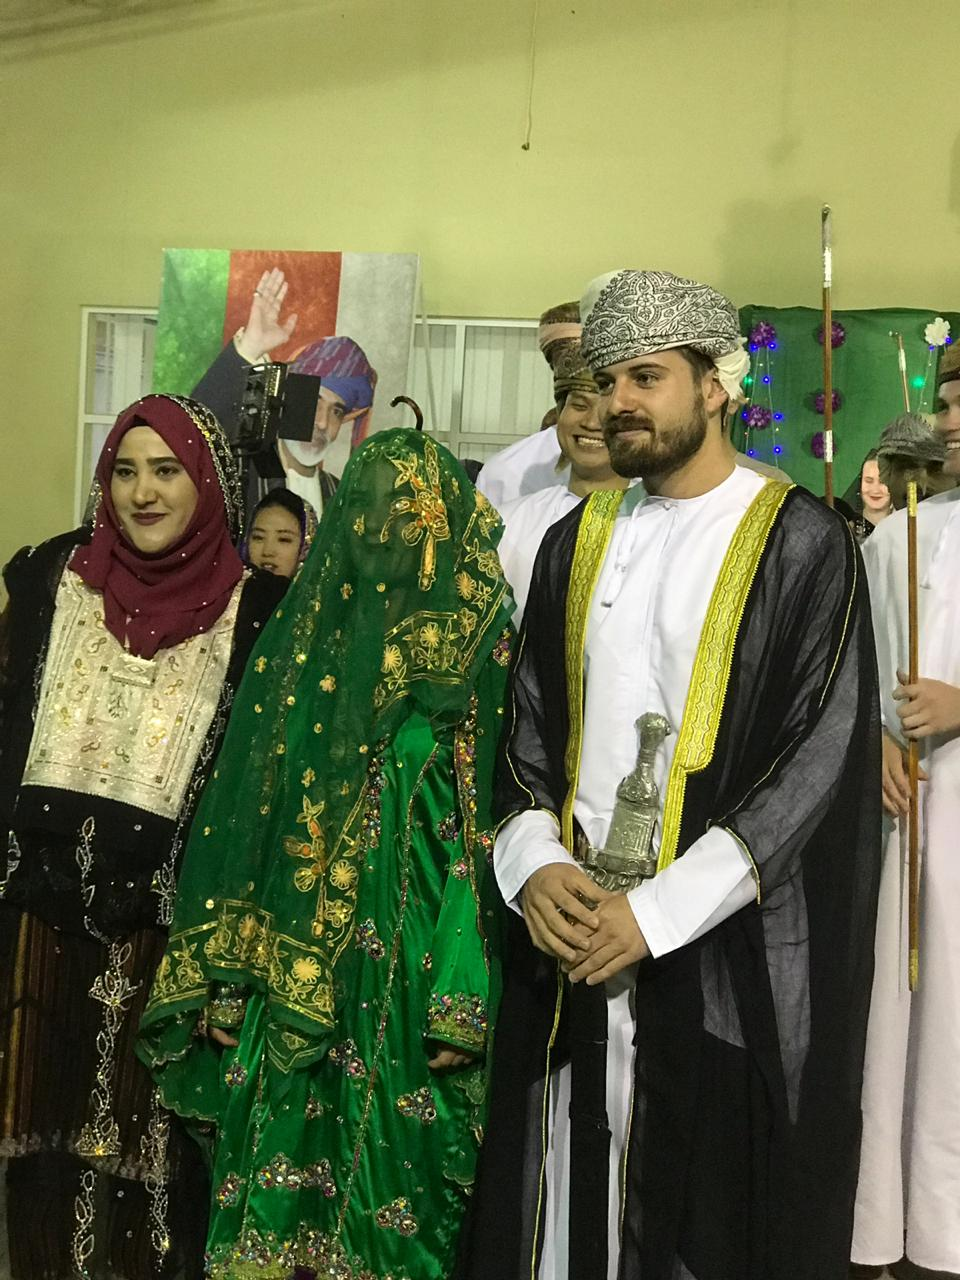
\includegraphics[width=8cm]{img/udo_clanky/Humr_oman.jpg}
\end{center}

Za prvé, všude jsou fotky SQ v různých pózách (sultán Qábús sedící, klečící, mávající, vzdávající se, usmívající se, važný, s holí a s mečem) a vše se tady jmenuje po SQ  - nemocnice, univerzity, školky, mešity, knihovny, lékárny, městské čtvrti - dokonce i na všech bankovkách je jen sultán. Oproti šíleným diktátorům a generálům jinde mají Ománci svého sultána rádi a neustále se usmívají… Také se k tomu váží příjemně časté oslavy narozenin Sultána, státních svátků, narozenin proroka, arabštiny a dalších příležitostných možností k tomu udělat si volno.

Za druhé, díky masivní výstavbě dálnic to tu vypadá jako v USA, akorát místo lánů kukuřice je kamenitá poušť a hory. Jako v USA to tu i funguje – bez auta a klimatizace se daleko nedostanete. Ve škole svádíme neustálý boj s učiteli o mukajjif (větrák), protože místní jsou nadšení z toho, když můžou vychladit místnost pod 20 stupňů. V kombinaci s venkovní teplotou to představuje smrtelné kombo.

Takový běžný Ománec (muž) nosí většinu svého života volné jednodílné pyžamo – říká se mu dišdáša – a je to oblek velmi pohodlný, a však nedá se v něm běhat, sedět nebo klečet – aniž by nebylo třeba ho vykasat. V práci se nosí masar nebo hamdáníja = šátek zavázaný do turbanu. Po práci už jen kumma – kastrolovitá čapka. Mladé Ománky jsou ovlivněné módou ze Zálivu a Saudské Arábie, takže ven vyráží zásadně celé v černém – hidžáb i abája - doma si ale nosí co chtějí. Jakmile jsou již dostatečně staré (bohužel jsem zatím nezjistil přesný věk zlomu – je to něco mezi 30 a smrtí), nosí tradiční, ultranazdobené a barevné oblečení. Vypadají pak jako noční můra všech epileptiků.

Když se Ománci potkají, následuje zhruba 1minutový rituál, během kterého si podají ruce, začnou třást, dotknou se nosem, navzájem se optají, co je nového a navzájem si odpoví, že vůbec nic. Až po rituálu se přejde na věc a můžou si říct, co že je tedy nového. 

Co se týče jídla, místní typická strava se skládá především z rýže, kuřete, datlí, rýže, humusu, datlí, zeleniny s kečupem, rýže, nánů(chlebových placek) a datlí a rýže. Pije se zásadně „šáj karak“, neboli přeslazená silná masala a káva s kardamomem a hřebíčkem. 

Jako všude jinde na Blízkém Východě, i zde si lidé váží nadmíru vody. Ománci jsou náležitě hrdí na svůj 3000 let starý systém „Afládž“ neboli zavlažovací kanály, které jsou zapsány na seznamu UNESCO (nyní vybetonované strouhy). To bohužel ale znamená, že hlavní atrakce veškerých výletů jsou vyschlá vádí, studny a kanály. Historie pevnosti netřeba, hlavně když je afládž…

Univerzita organizuje nejen vyučování, ale i program kulturní – krom návštěvy mnoha pevností (pokud někdy zamíříte do Ománu, stačí vidět jen jednu – např. pevnost Nizwa) jsme zatím například fandili při závodech velbloudů(kvůli vedru se závodí ráno v půl šesté nebo pozdě večer), smlouvali na trzích o věci vyrobené v Číně, oblékali se do tradičního oblečení nebo plavali ve vádí. 

Celkově si vlastně nemůžu stěžovat –starají se tu o mě pěkně, objevuji další kus světa, v rámci kulturní akce jsem se stihl poprvé oženit a trénuju arabštinu – pro studenty obzvlášť výhodné. 

\podpis{Humr}
\subsection*{Hra po Praze 2019 z pohledu organizátorů}
\label{sub:hra_po_praze_2019_z_pohledu_organizátorů}

Letošní Hra po Praze byla ta nejsofistikovanější, nejpřipravovanější a z realizační stránky i nejtěžší hra z těch tří, co jsem zatím dělala. První porada proběhla 14.10. a od té doby jsme měli další čtyři porady a jednu přespávačku. Celkově se na vymýšlení a organizaci podílelo devět uďů a mnoho dalších bylo na místě. Celý měsíc a půl jsme intenzivně vymýšleli zápletku, sháněli materiály, verbovali externisty… zkrátka přípravám jsme věnovali mnoho času.

Co se týče samotné realizace HpP, možná jsme si dali příliš málo času pro realizaci na místě (proto někteří patroni přišli pozdě na sraz skupinek), takže byl začátek poměrně zmatený a hektický. Já osobně jsem se nervovala úplně maximálně, hih. Celou dobu jsme byli v lehkém časovém skluzu, ale nakonec jsme jej dohnali, takže zakončující bitva vyšla přesně, za což jsem byla já osobně velmi ráda. 

Ale i tak - přes veškerý stres a strach z neúspěchu nebo úplného sesypání hry - se Hra dle mého názoru vydařila a věřím, že si ji děti i spousta uďů užilo. Což považuju za nejlepší výsledek, jaký mohl nastat.


\begin{center}

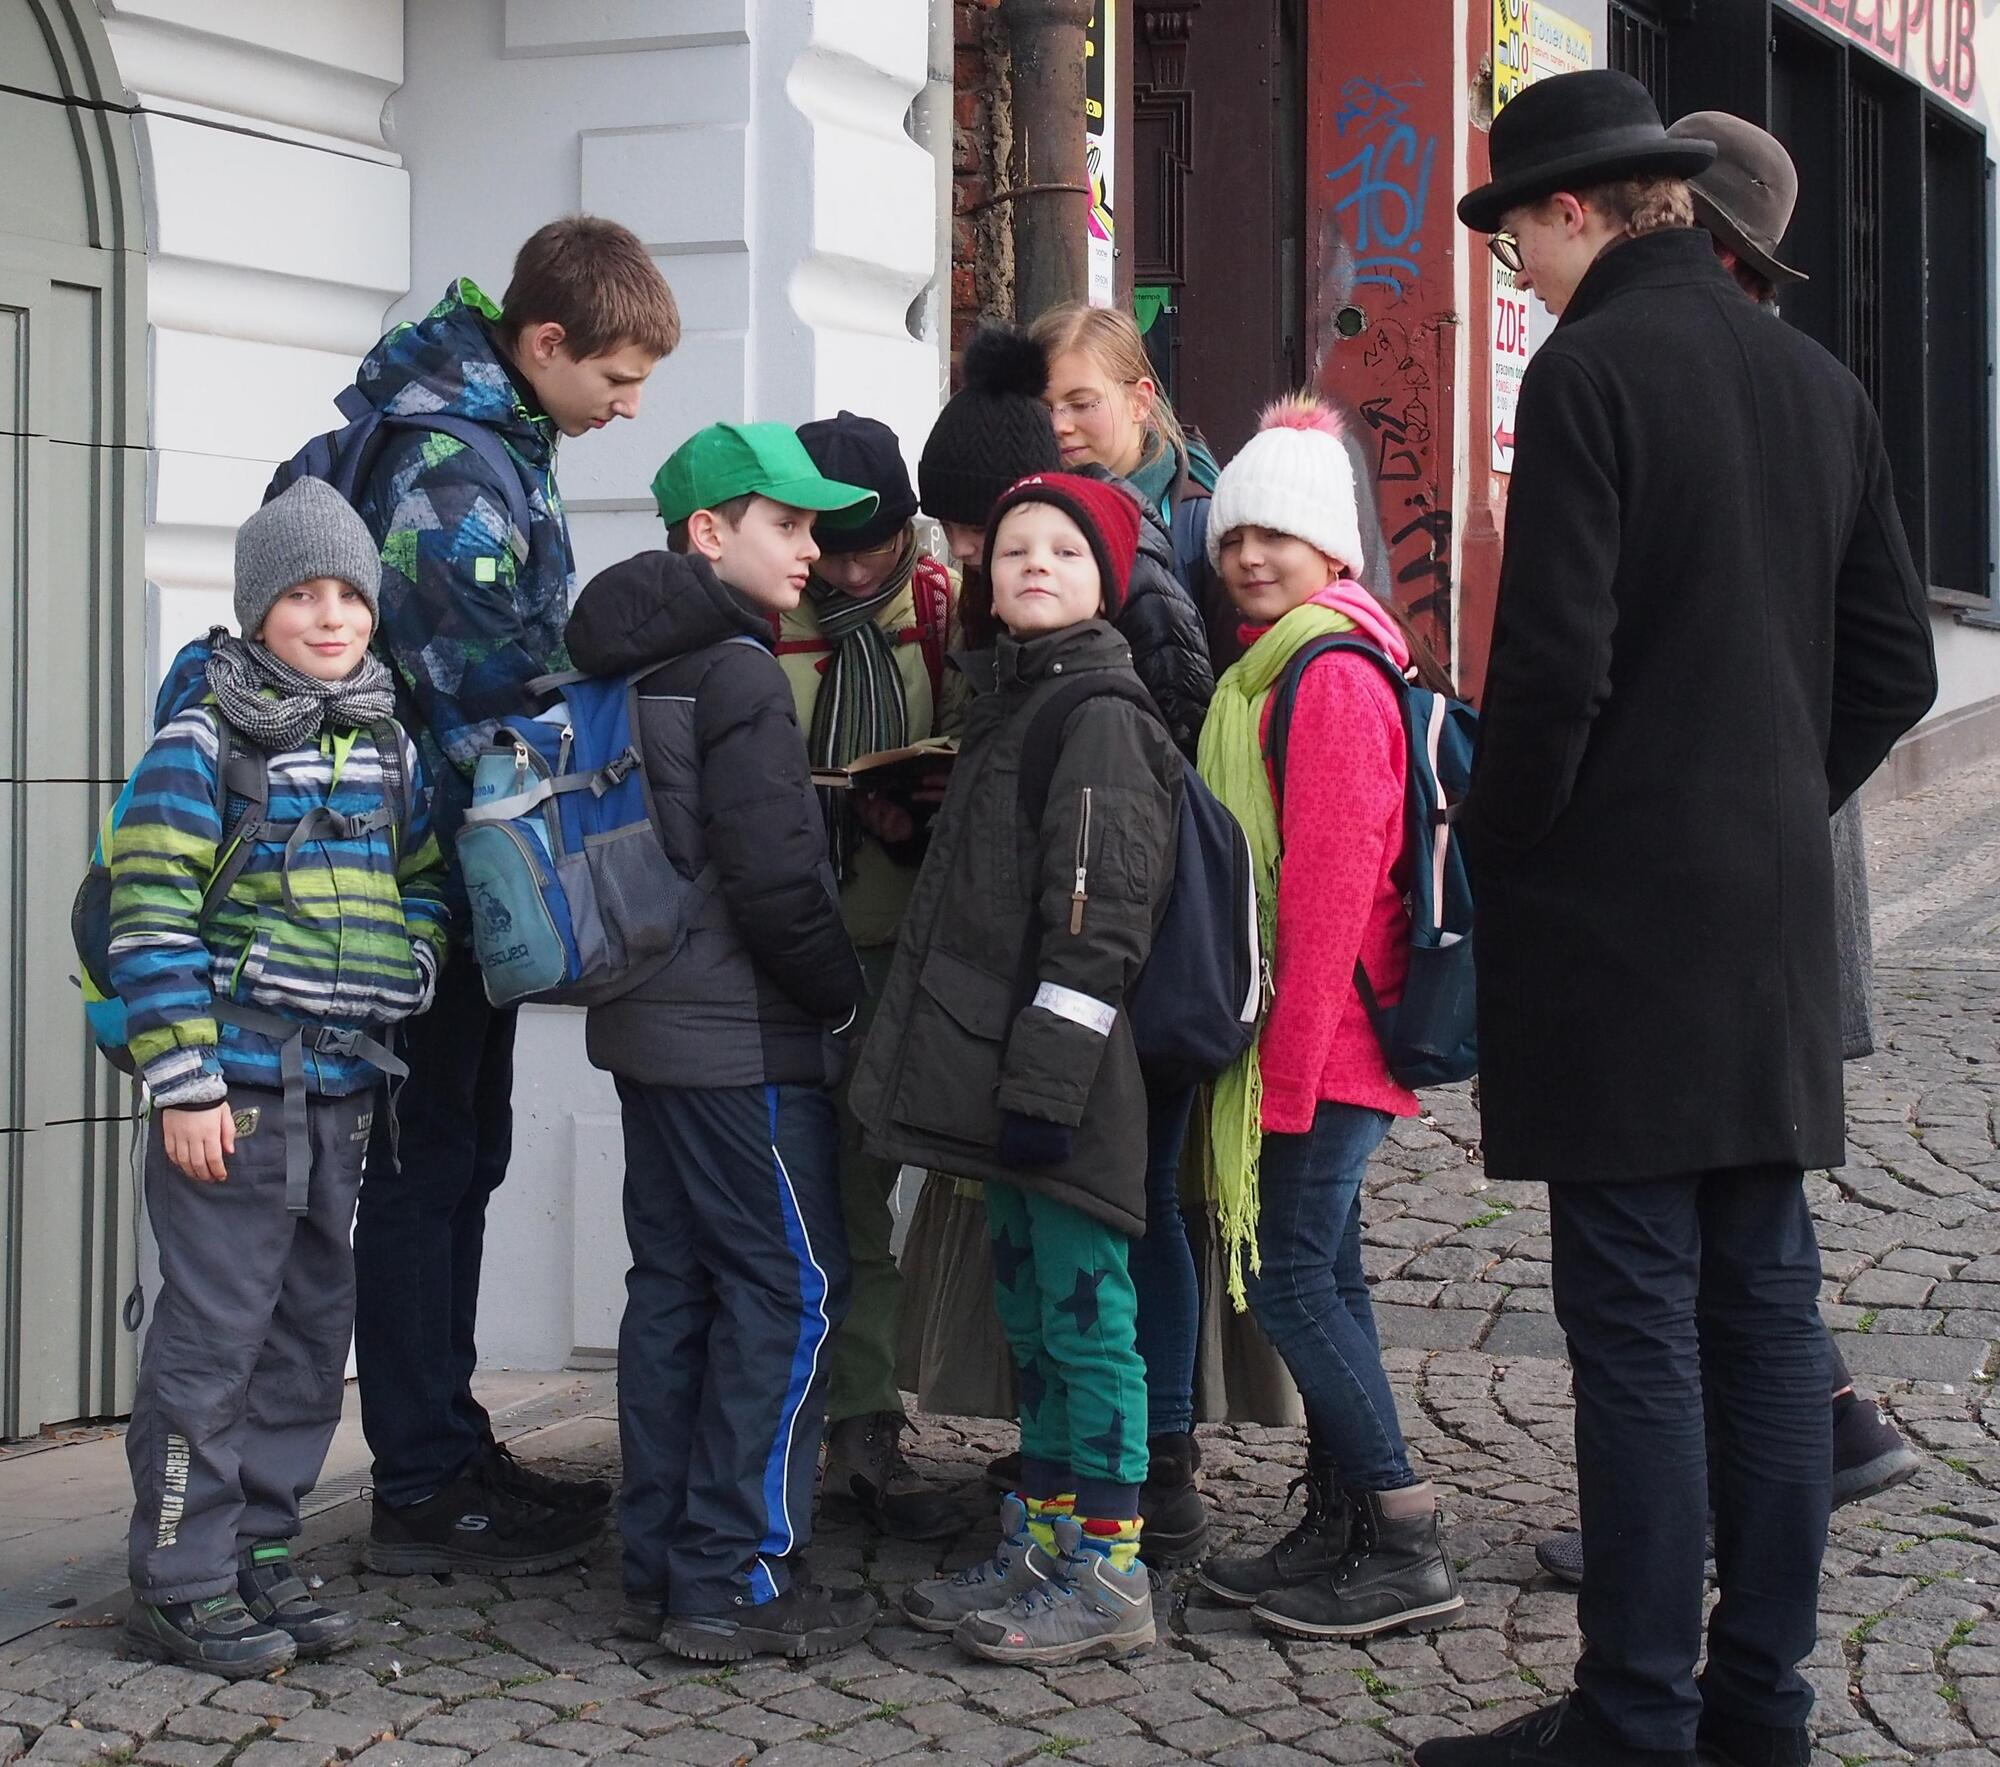
\includegraphics[width=8cm]{img/udo_clanky/hrapopraze.JPG}

\end{center}
\podpis{Štípadlo}
\clearpage

\clearpage
% chapter udove (end)

\chapter{Hory 2019 - Mařenice} % (fold)
\label{cha:hory}
\begin{wrapfigure}[8]{r}[1em]{3cm}
	\centering
	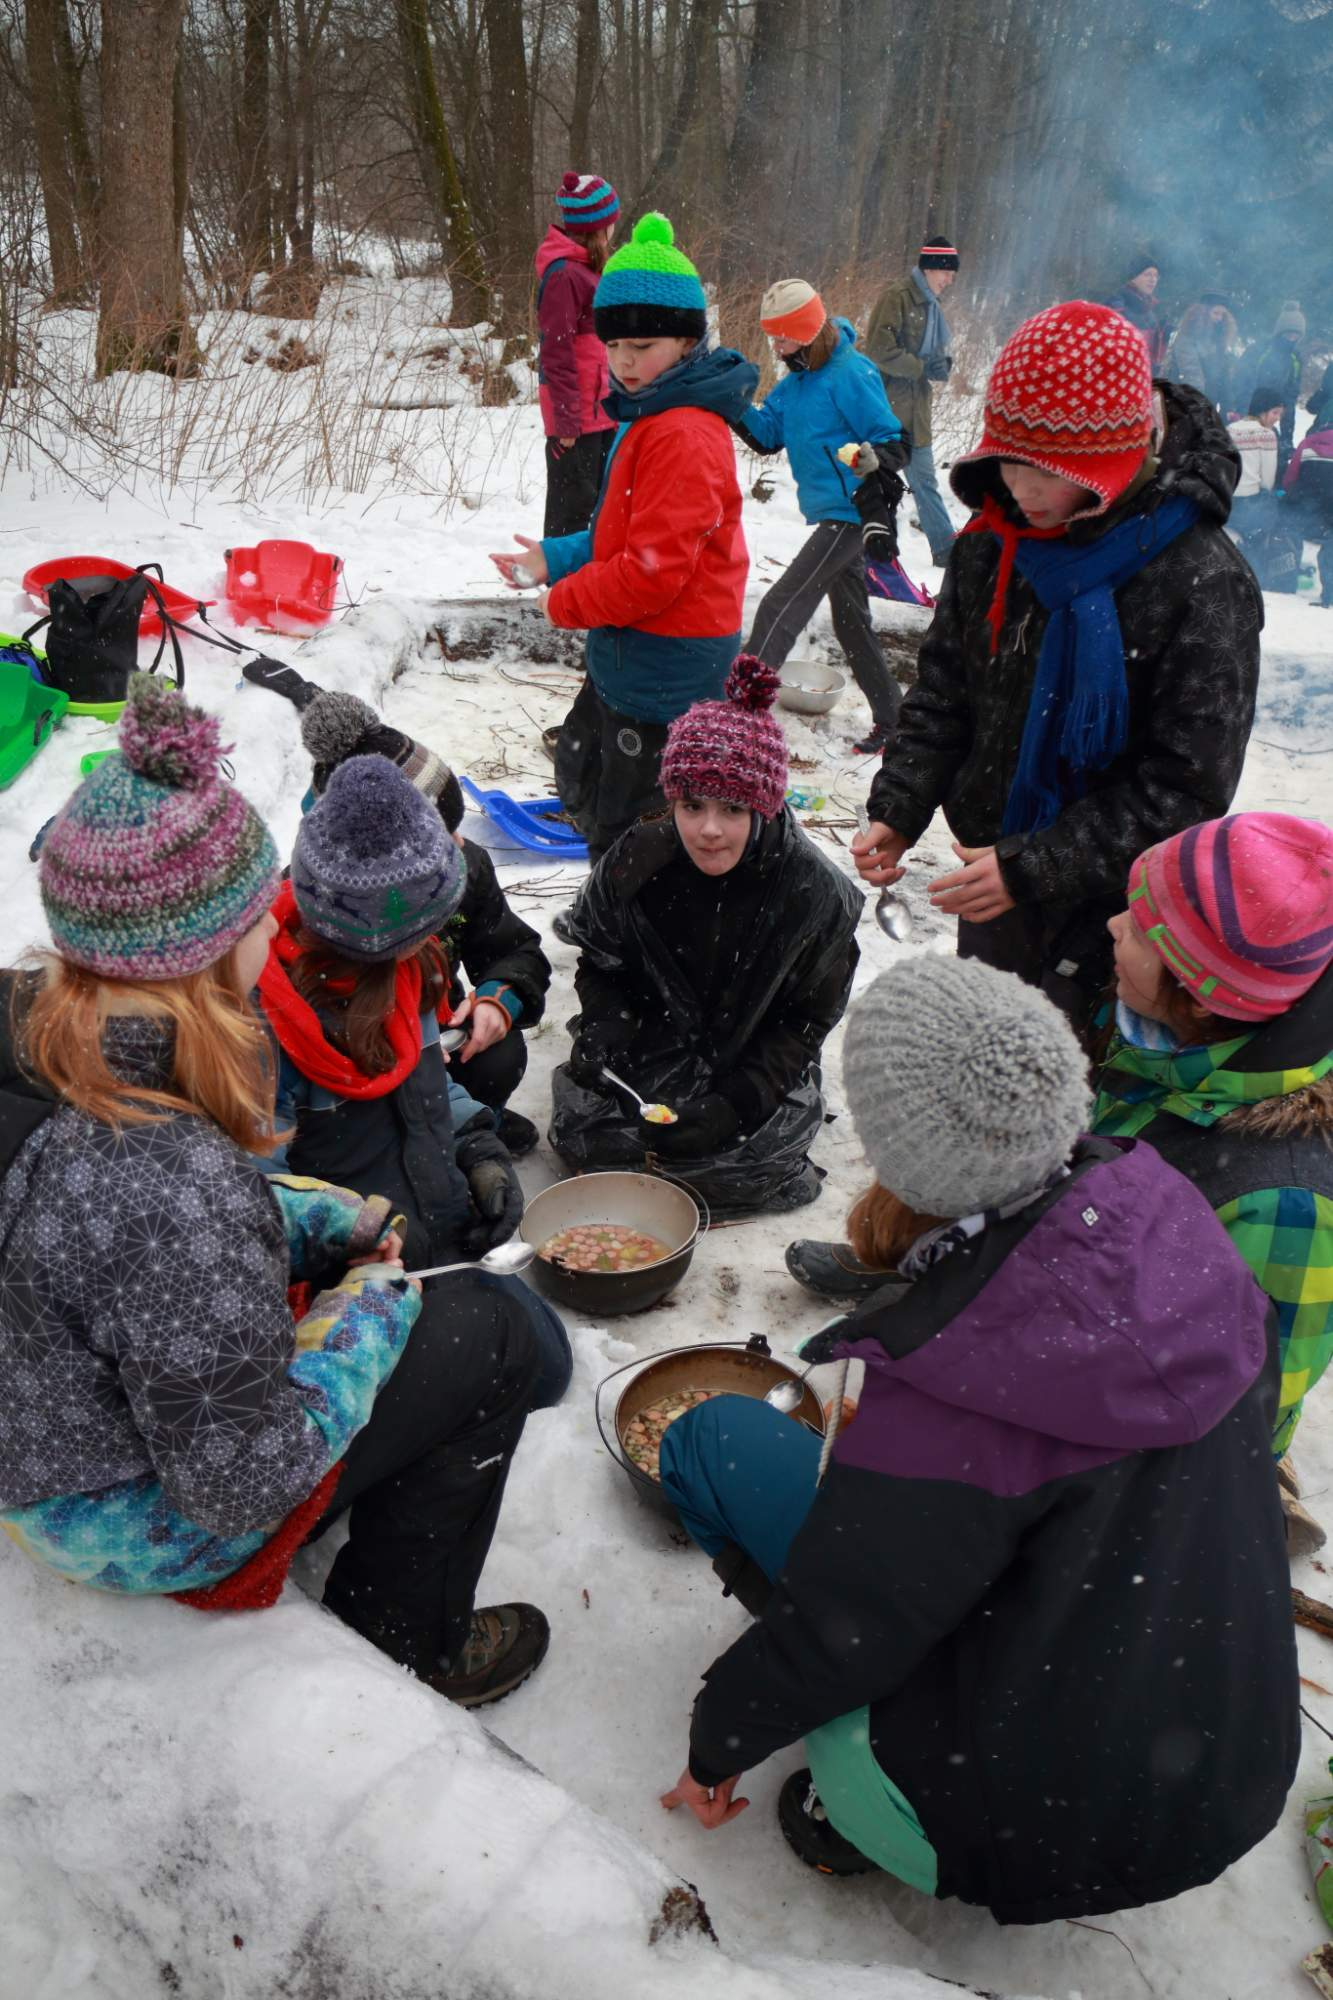
\includegraphics[width=3cm]{img/hory/jidlo.jpg}
\end{wrapfigure}
Hory byly už dávno, předávno. Tak dávno, že ty další jsou až nebezpečně blízko. Ale to nevadí, protože hory, to je především pohoda! Takže zatímco oko se kochá fotkami z hor minulých, dušička může poposkočit a zaplesat, že ty nadcházející jsou už skoro za dveřmi!


\begin{center}

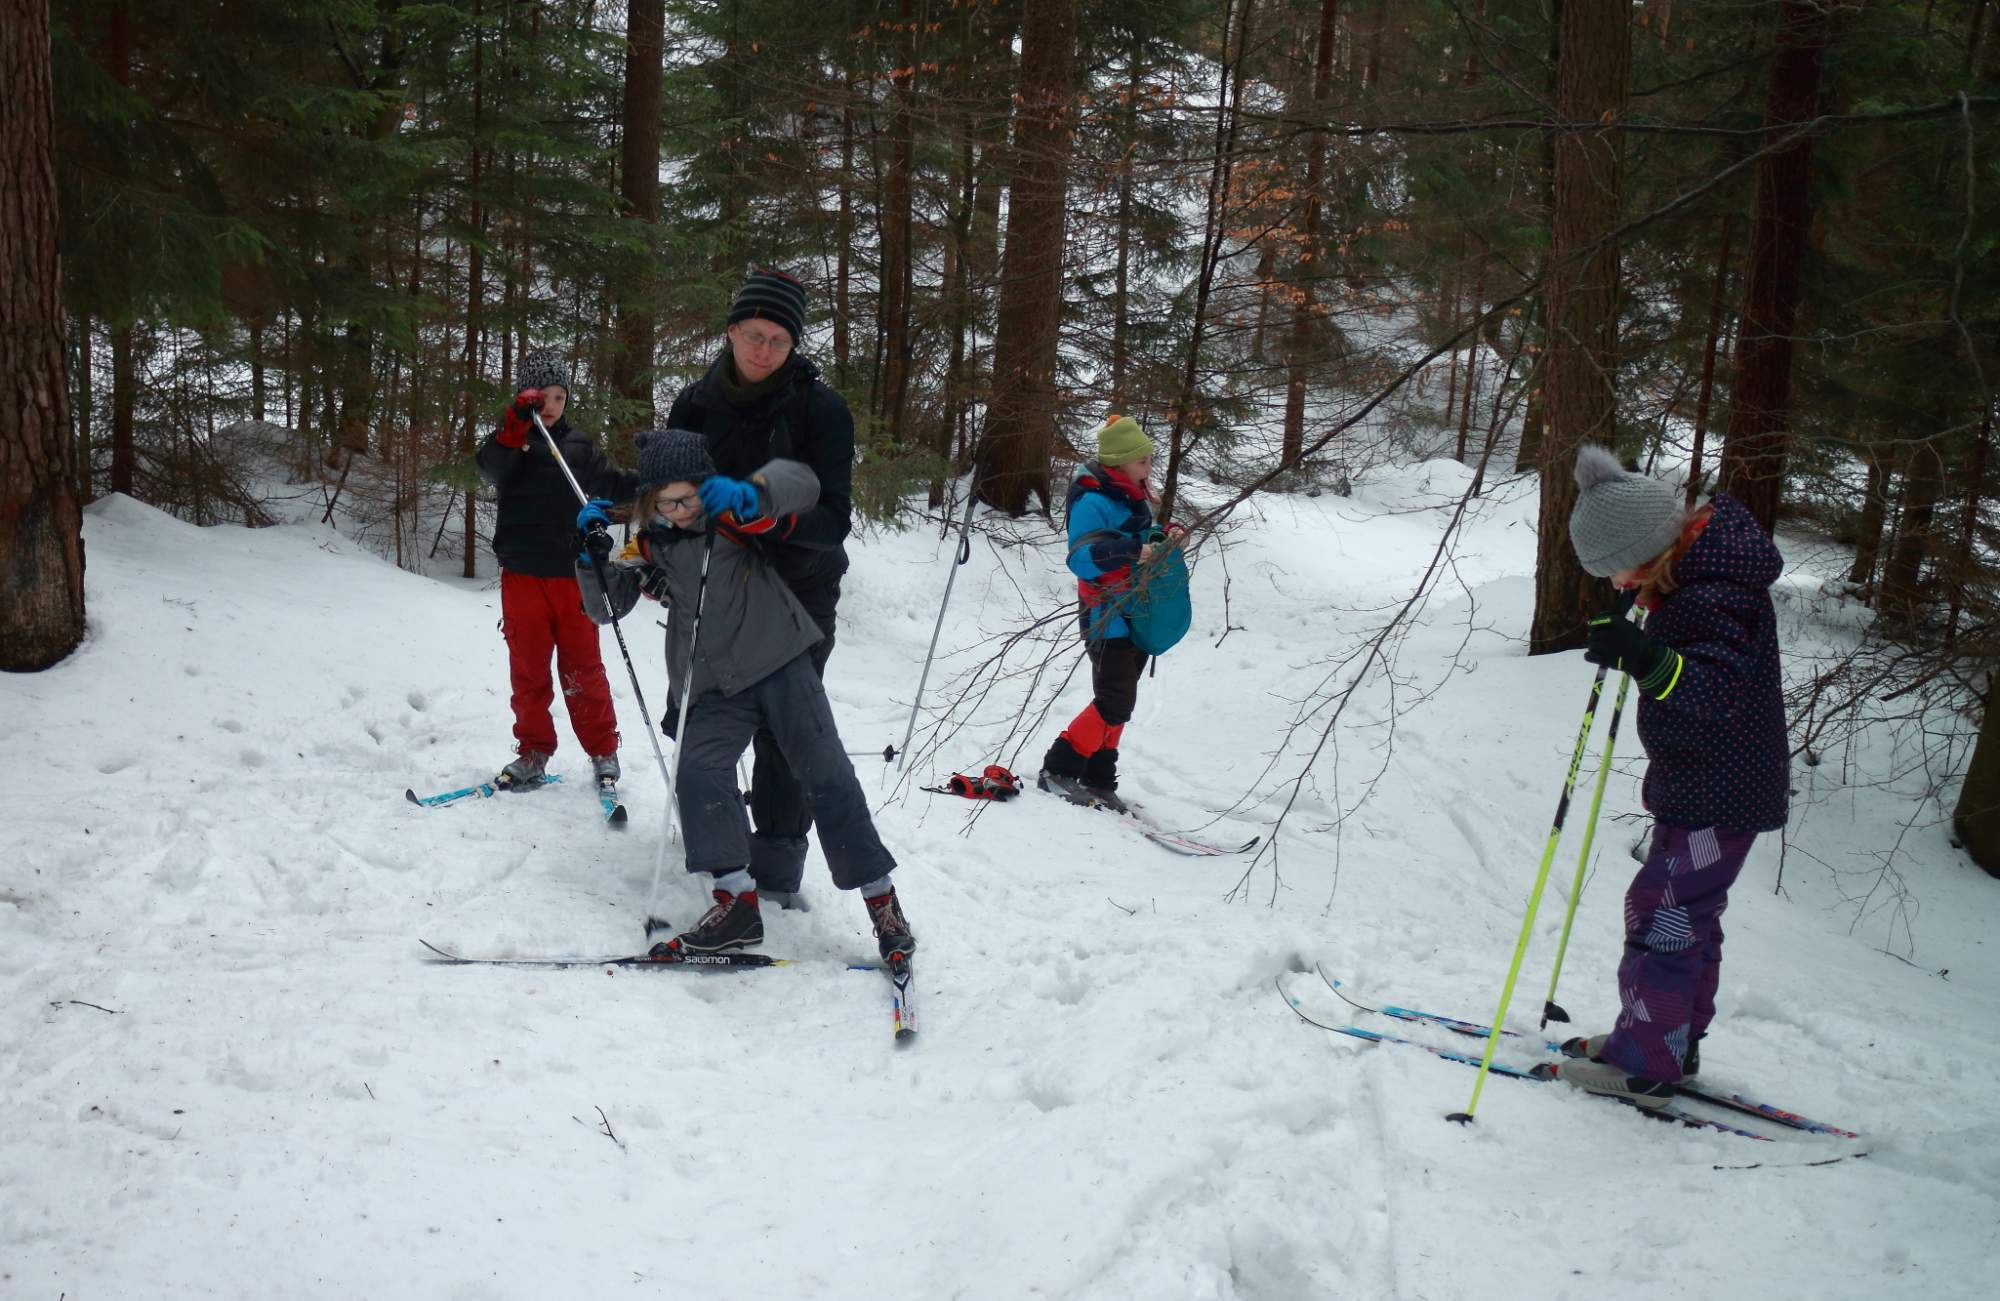
\includegraphics[width=9cm]{img/hory/lyze.jpg}
\end{center}

\vspace{5mm}

\begin{center}
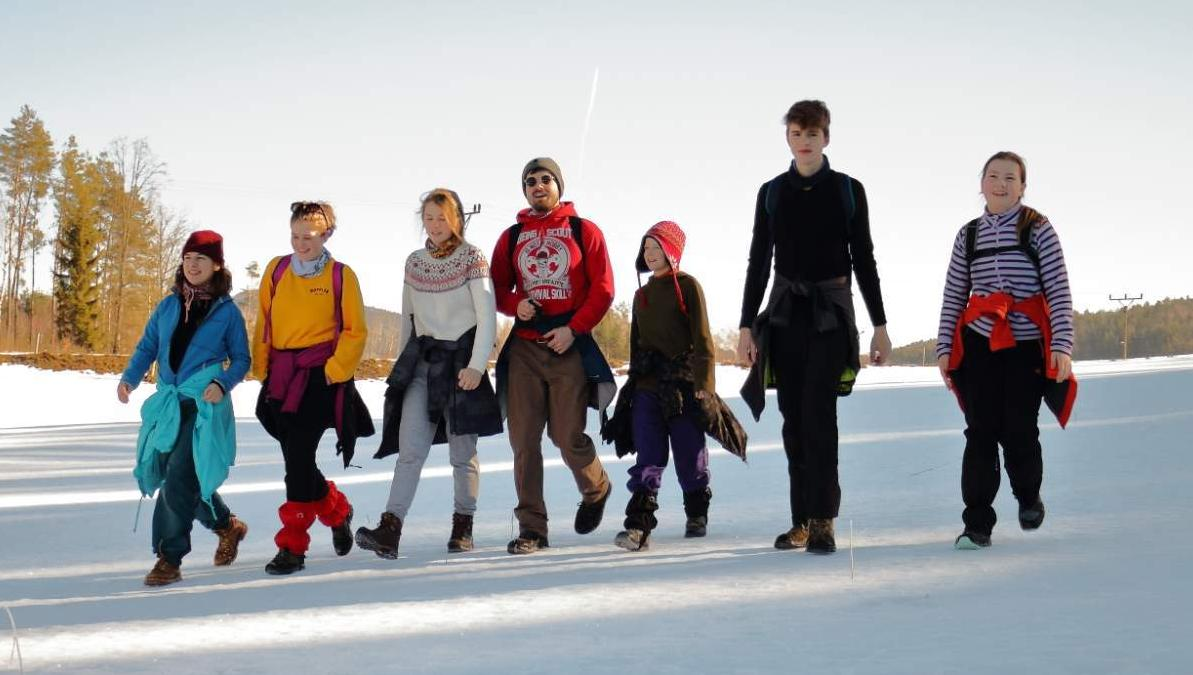
\includegraphics[width=12cm]{img/hory/drsnaci.jpg}
\end{center}



% chapter hory_2019_mařenice (end)
\clearpage

\chapter{Projekt: Středisko Keya 2021} % (fold)
\label{cha:projekt_středisko_keya_2021}

Pro někoho to možná bude úplnou novinkou, pro jiného potvrzením spekulací, a někdo to třeba už dávno věděl, každopádně přišel čas na to vyslat tuto informaci oficiálně do světa – na přelomu roku 2020 a 2021 se oddíly Anpetu a Hanyetu oddělí od Blaníku a dají vzniknout samostatnému středisku Keya.

Je to informace, která může znít poměrně převratně, nicméně faktem je, že pro většinu zúčastněných o nějaký velký převrat nejde. Členové oddílů ani jejich rodiče pravděpodobně nepoznají rozdíl, alespoň půjde-li vše tak, jak doufáme. Největší změna to tak bude pro samotné vedoucí v oddílech, pro které se změní ledasco, ovšem snad jenom k lepšímu.

Jak jsme k rozhodnutí o této na první pohled možná kosmetické změně dospěli? Naším primárním důvodem je skutečnost, že Blaník se svými stovkami členů se nám čím dál více stával finančním a technickým správcem a přestával být skautskou rodinnou. Ono udržovat vztahy s patnácti dalšími oddíly rozesetými po celé Praze zkrátka a dobře není v lidských silách. Po loňském rozdělení Keyi na dva oddíly se pro nás navíc stalo mnohem důležitějším udržet úzké vazby hlavně mezi sebou. A když se k tomu přidá skutečnost, že máme vlastní klubovnu a objevila se skupina zkušených vedoucích, kteří jsou ochotní se budoucímu středisku Keya věnovat, nic nebrání tomu, abychom se do zakládání pustili.

Jak to bude celé probíhat? V uplynulém roce probíhaly diskuse o tom, jakým způsobem bychom chtěli, aby naše středisko fungovalo. Tyto diskuse se stanou základním kamenem práce vznikajícího střediskového vedení. Zároveň jsme se domluvili s vedením Blaníku na jízdním řádu „Kexitu“ – během jara zkompletujeme tým vedení střediska, od příštího skautského roku (to je od podzimu 2020) začneme fungovat nezávisle na Blaníku, a s novým rokem kalendářním dojde i k oddělení právnímu a finančnímu.

\begin{center}
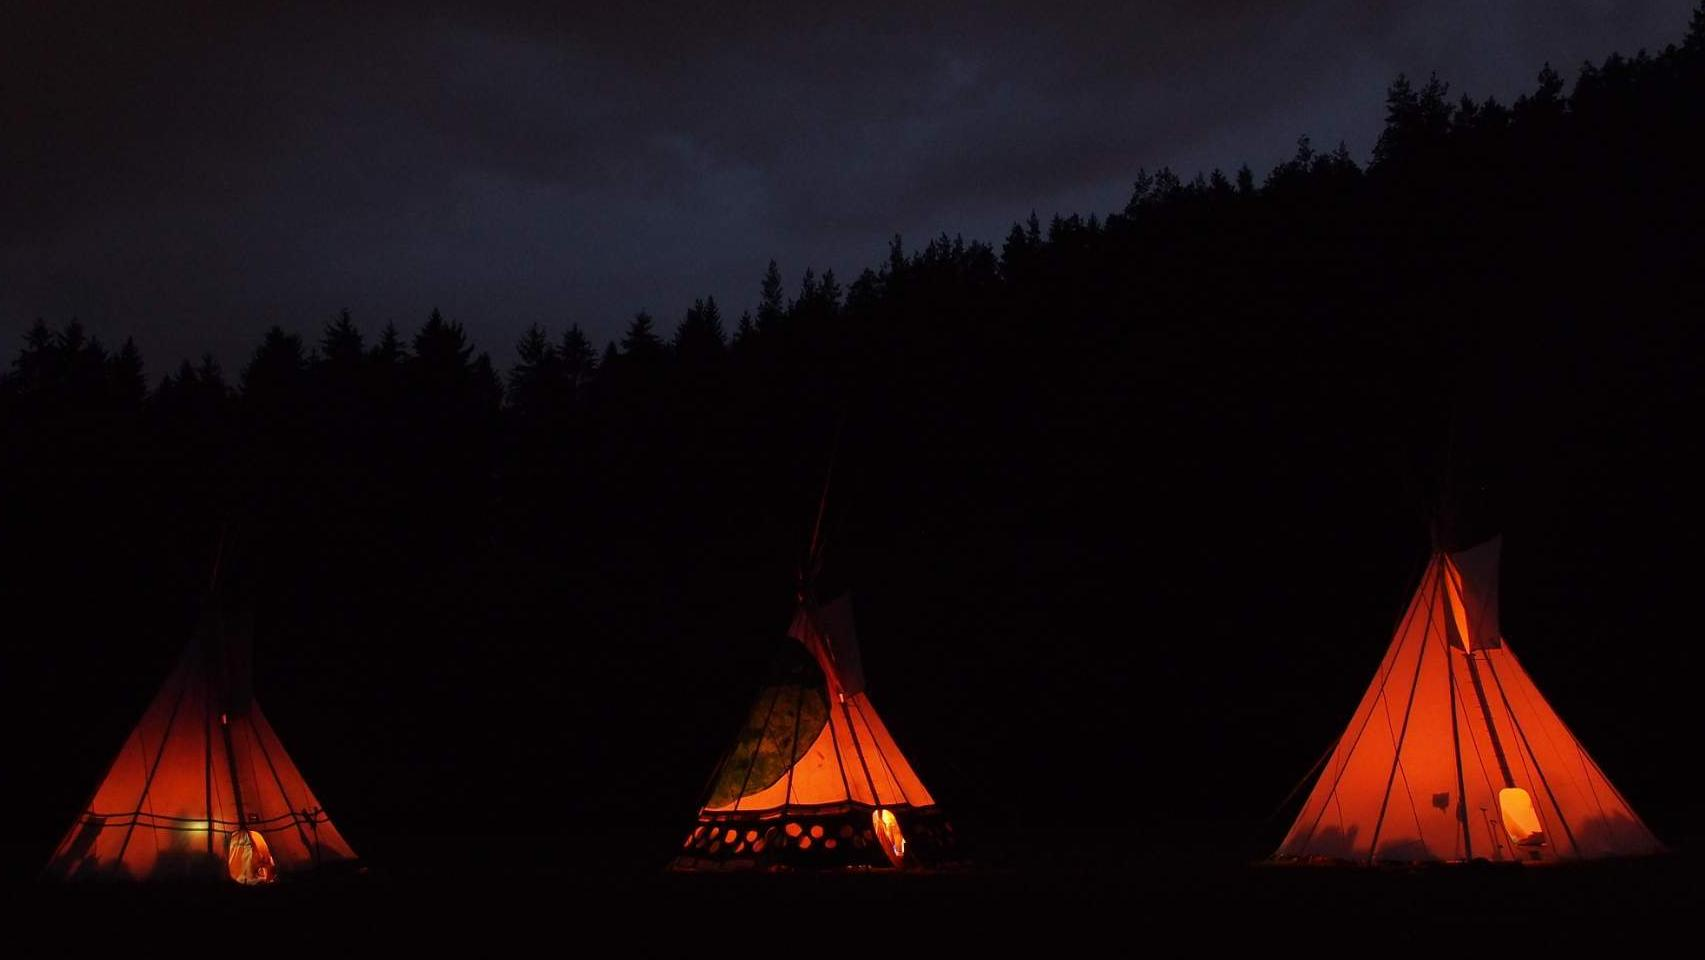
\includegraphics[width=9cm]{img/udo_clanky/fikuv_clanek_stredisko.jpg}
\end{center}

Dobrou zprávou je, že se celý projekt nese v pozitivním duchu. Naše oddělení není vynucené a ani k němu nedochází z důvodu, že bychom měli nějaké spory s Blaníkem. Věříme sice, že v užším kruhu se nám bude lépe dařit udržovat vzájemné vztahy a budeme snad i fungovat o něco efektivněji, ale rozhodně neodcházíme ve zlém či s pocitem povýšenosti. Spíše na to všechno hledíme jako na výzvu, která nám jistě přinese mnohé problémy a komplikace, ale na kterou se s chutí vrhneme. Tak nám držte palce, budeme to potřebovat!

\podpis{Fík}

\clearpage

% chapter projekt_středisko_keya_2021 (end)

\chapter{Křížovka} % (fold)
\label{cha:křížovka}

\begin{center}

\vspace{-20pt}

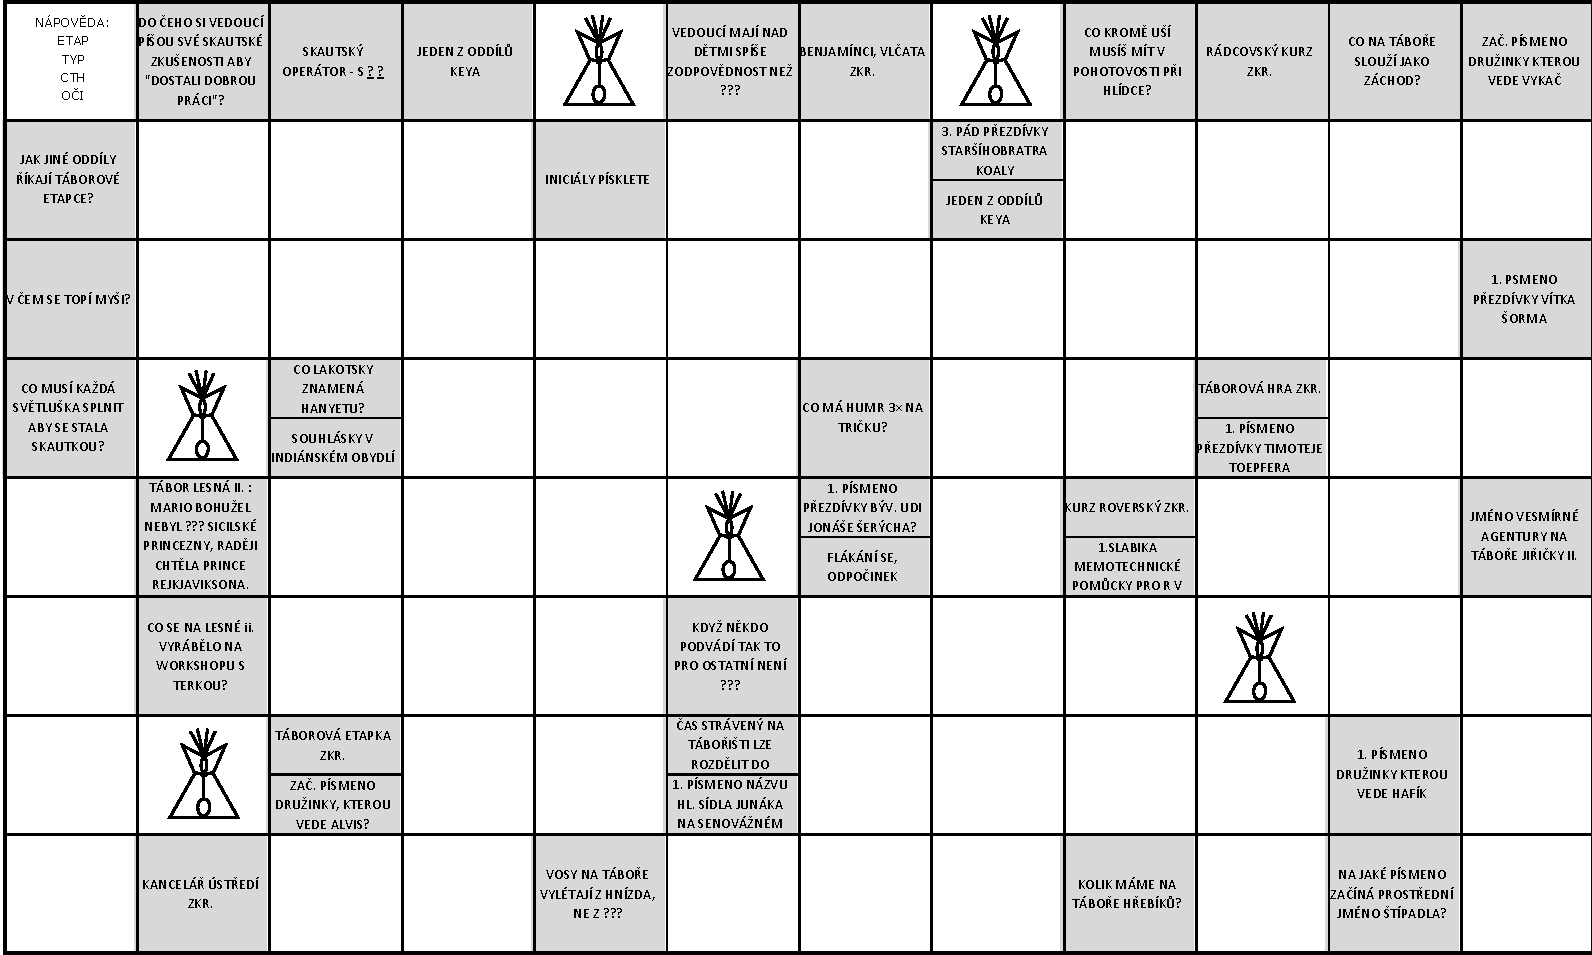
\includegraphics[angle=270,origin=c,height=0.7\textheight]{img/krizovka.pdf}
\end{center}
% chapter křížovka (end)

\chapter{Statistické okénko}
\label{statistika}

\begin{center}

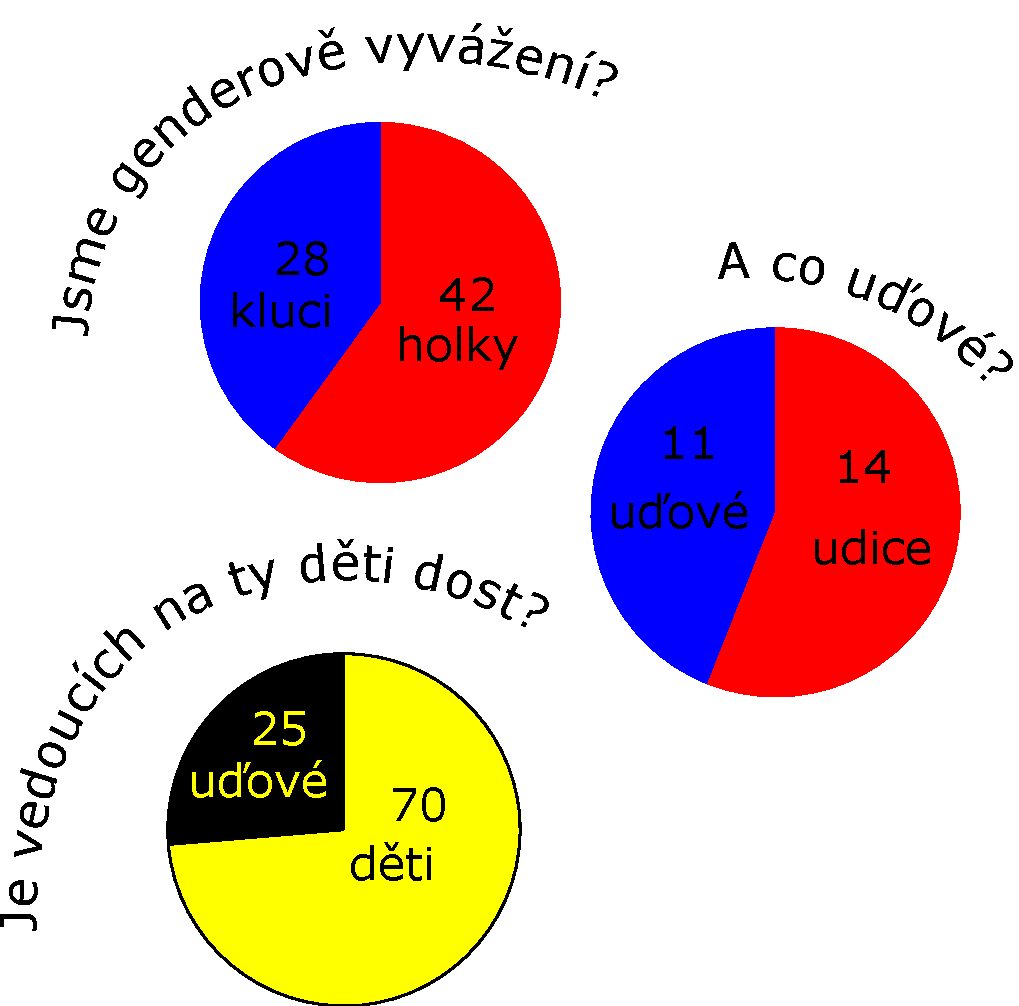
\includegraphics[width=12cm]{img/statistika/grafy-kolacove.pdf}

\end{center}


\clearpage

Pro ještě větší milovníky statistiky přikládáme analýzu věku a doby členství v oddíle zpracované jako histogramy. Na Obr. \ref{fig:vek} je rozdělení věku (platné jeden týden před vánočním večírkem). Na Obr. \ref{fig:clen} je rozdělení počtu let v oddíle.

Pro upřesnění: roky počítáme od nuly. Data pochází ze skautisu, nepřesnosti jsou (obvláště u nových členů) možné. Grafy jsou na ose x zaříznuté a neobsahují tedy všechny hodnoty (někteří exuďové 24 let v oddíle). V těchto histogramech nebyli rozlišeni uďové od dětí.

\begin{figure}[!ht]
  \begin{center}
    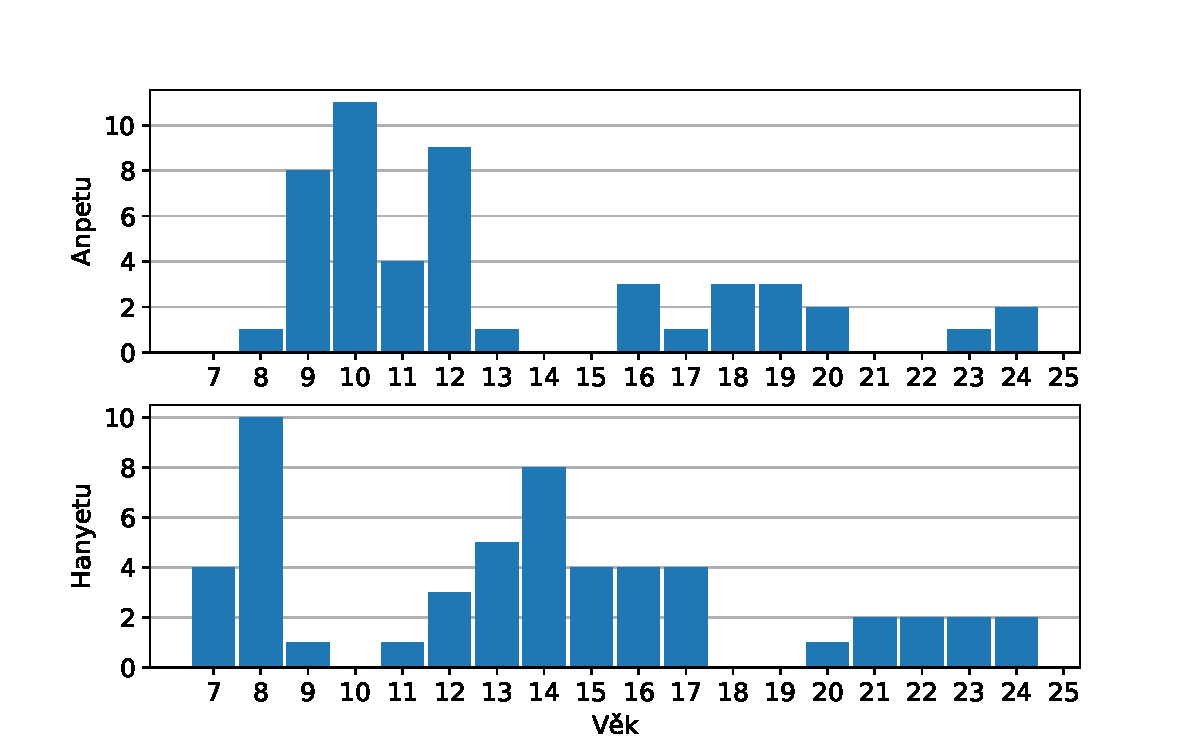
\includegraphics[width=0.75\textwidth]{statistika/hist_vek.pdf}
  \end{center}
  \caption{Histogram věku účastníků}
  \label{fig:vek}
\end{figure}


\begin{figure}[!ht]
  \begin{center}
    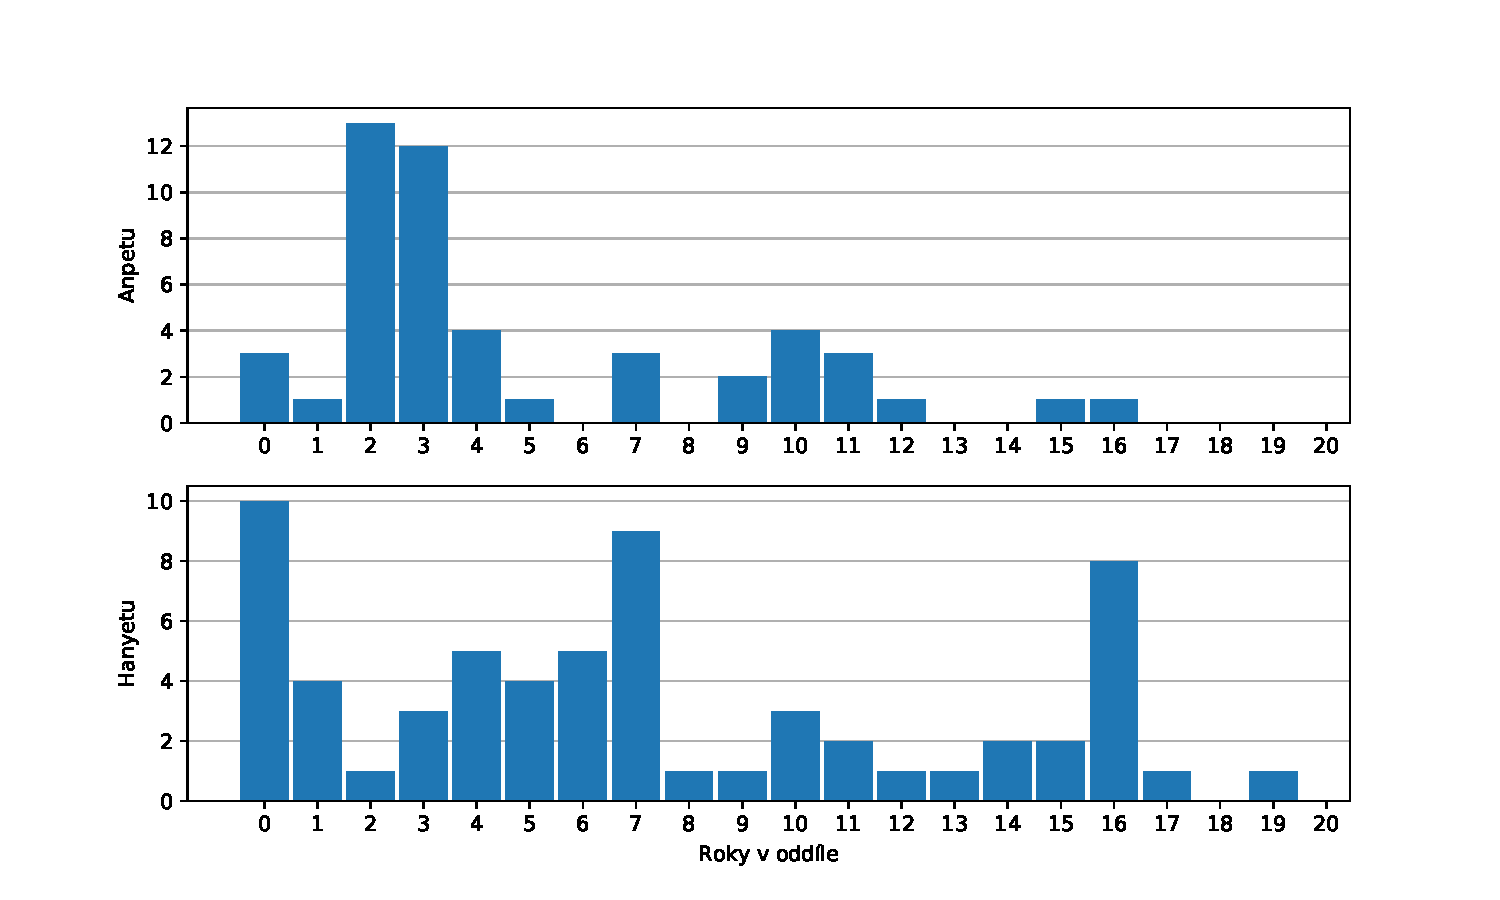
\includegraphics[width=0.75\textwidth]{statistika/hist_clen.pdf}
  \end{center}
  \caption{Histogram doby člesntví v oddíle}
  \label{fig:clen}
\end{figure}

\clearpage


\chapter{Víte, že…?} % (fold)
\label{cha:vite}
	
\begin{itemize}
	\item jsme opět zazářili na Jupijou? V kategorii světlušky a vlčata vybojovaly Eskymáci 2. místo, v kategorii skautů a skautek získaly Ještěrky 3. místo a kategorii roverů a rangers se umístili Lemuři jako 1.

	\item měl Kámen svatbu?
	\item během září se uskutečnil rekordní počet porad?
	\item z letošního Anpetího tábora odjížděli všichni účastníci se žlutým šátkem, kdežto z Hanyetího tábora odjížděli všichni účastníci s hnědým šátkem?
	\item se od konce tábora uskutečnily již 2 výjezdy na hledání tábořiště?
	\item v září vznikla nová Hanyetí holčičí skupinka, která už má jméno? Jmenují se Pandakaty, je jich 9 ve věku 6-8 a vede je Morče, Štípadlo a Šárka.
	\item úspěšně pokračuje kolaudace klubovny a je velmi pravděpodobné, že příští rok budeme mít kolaudačku?
	\item na letošní Hře po Praze kromě 41 dětí, 20 uďů taky 9 externistů?

\end{itemize}
% chapter vite (end)

\clearpage

\chapter{Okénko pro partnery} % (fold)
\label{cha:okénko_pro_partnery}

\begin{center}

\includegraphics[width=10.5cm]{img/VAPP.pdf}
\vspace{5mm}


\includegraphics[width=10.5cm]{img/maunfaktura.pdf}

\end{center}
% chapter okénko_pro_partnery (end)

\clearpage

\clearpage

\chapter{Slovo závěrem} % (fold)
\label{cha:slovo_závěrem}

Závěrem se hodí poděkovat všem, bez kterých by tato Kniha Keya nevznikla. Velký dík patří tedy přispěvatelům, ať už dětem nebo Uďům, kteří namáhali své mozkové závity, zavzpomínali a stvořili příspěvek, bez kterých by byla kniha poněkud prázdná. Všechny příspěvky jsou zaznamenány bez úprav tak, jak autor svou myšlenku zachytil. (Nutno říci, že luštění některých příspěvků bylo značně zapeklité.)

Další díky patří všem fotografům, kteří na akcích často nasazují své životy a hlavně své drahé aparáty, abychom mohli po návratu vzpomínat, jakou že to běhačku jsme si zahráli. Bez jejich fotek by kniha byla nevesele nebarevná.
Stojí za to poděkovat (tisk+vazba)
A veliké dlouhé hmmm si zaslouží hvězdný KKtým, tedy jmenovitě Kibitz, Koala, Morče, Pískle, Štípadlo, Vykač a taktéž Špunt za to, že do toho šli a že to dotáhli a to v rekordním čase.

Díky!


\begin{center}
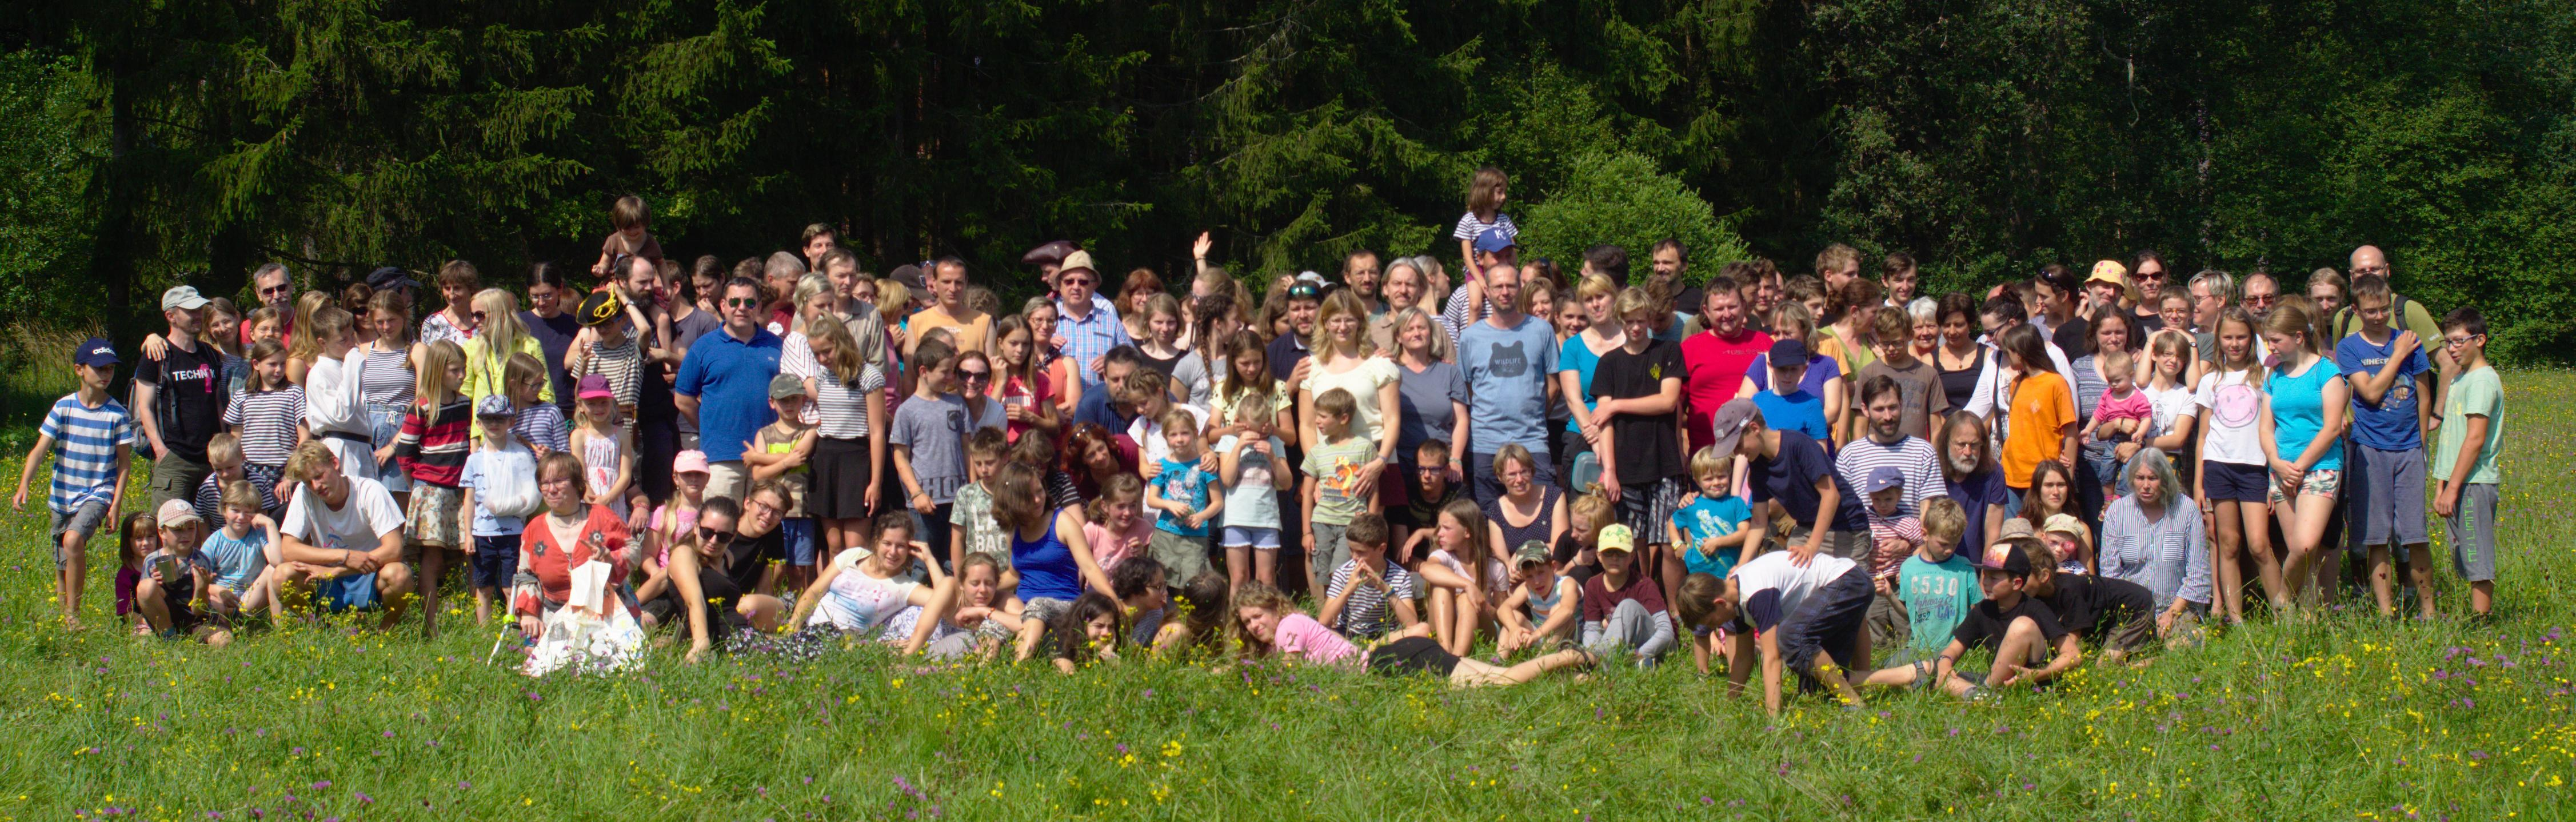
\includegraphics[width=\textwidth]{img/vsichni.jpg}

\includegraphics[width=\textwidth]{img/QR/komplet.pdf}
\end{center}

% chapter slovo_závěrem (end)
\end{document}